
% \documentclass[english]{fitthesis} 
\documentclass[english,zadani]{fitthesis}
%---rm---------------
\renewcommand{\rmdefault}{lmr}%zavede Latin Modern Roman jako rm / set Latin Modern Roman as rm
%---sf---------------
\renewcommand{\sfdefault}{qhv}%zavede TeX Gyre Heros jako sf
%---tt------------
\renewcommand{\ttdefault}{lmtt}% zavede Latin Modern tt jako tt

% disables function of the template which replaces quotation marks
% to avoid unnecessary replacements in the API descriptions etc.
\csdoublequotesoff

\usepackage{url}

% =======================================================================
% "hyperref" package create clickable links in pdf if you are using pdflatex.
% Problem is that this package have to be introduced as the last one so it 
% can not be placed in the template file.
\ifWis
\ifx\pdfoutput\undefined % we are not using pdflatex
\else
  \usepackage{color}
  \usepackage[unicode,colorlinks,hyperindex,plainpages=false,pdftex]{hyperref}
  \definecolor{hrcolor-ref}{RGB}{223,52,30}
  \definecolor{hrcolor-cite}{HTML}{2F8F00}
  \definecolor{hrcolor-urls}{HTML}{092EAB}
  \hypersetup{
	linkcolor=hrcolor-ref,
	citecolor=hrcolor-cite,
	filecolor=magenta,
	urlcolor=hrcolor-urls
  }
  \def\pdfBorderAttrs{/Border [0 0 0] }  % bez okrajů kolem odkazů / without margins around links
  \pdfcompresslevel=9
\fi
\else % pro tisk budou odkazy, na které se dá klikat, černé / for the print clickable links will be black
\ifx\pdfoutput\undefined %  we are not using pdflatex
\else
  \usepackage{color}
  \usepackage[unicode,colorlinks,hyperindex,plainpages=false,pdftex,urlcolor=black,linkcolor=black,citecolor=black]{hyperref}
  \definecolor{links}{rgb}{0,0,0}
  \definecolor{anchors}{rgb}{0,0,0}
  \def\AnchorColor{anchors}
  \def\LinkColor{links}
  \def\pdfBorderAttrs{/Border [0 0 0] } %  without margins around links
  \pdfcompresslevel=9
\fi
\fi
% This solves the problems with links which leads after the picture
\usepackage[all]{hypcap}
\usepackage{listings}
\usepackage{fvextra}
\usepackage{subcaption}
\usepackage{algorithm}
\usepackage{algpseudocode}
\DefineVerbatimEnvironment{Verbatim}{Verbatim}{breaklines=true, breakanywhere=true}


% Information about the thesis
%---------------------------------------------------------------------------
\projectinfo{
  project={DP},
  year={2025},
  date=\today,
  %thesis title
  title.cs={Efektivní trénování neuronových sítí pro automatické rozpoznávání řeči},  % thesis title in czech language
  title.en={Effective Training of Neural Networks for Automatic Speech Recognition}, % thesis title in english
  %Autor / Author
  author.name={Matej},   %  author name
  author.surname={Horník},   %  author surname 
  %author.title.p={Bc.}, % title before the name (optional)
  %author.title.a={Ph.D.}, % title after the name (optional)
  %Ustav / Department
  department={UPGM}, % fill in appropriate abbreviation of the department according to assignment: UPSY/UIFS/UITS/UPGM
  % supervisor
  supervisor.name={Alexander},   %  supervisor name 
  supervisor.surname={Polok},   %  supervisor surname
  supervisor.title.p={Ing.},   % title before the name (optional)
  supervisor.title.a={},    % title after the name (optional)
  % keywords
keywords.cs={automatické rozpoznávanie reči, hlboké učenie, transformer modely, modely kódovač-dekóder, predtrénované modely, parametricky efektívne doladenie, PEFT, LoRA, DoRA, adaptéry, inicializačné stratégie, Wav2Vec2, BART, slovná chybovosť, WER, učenie typu sekvencia-na-sekvenciu, učenie s vlastným dohľadom, krížová pozornosť, doladenie, LibriSpeech, VoxPopuli, výpočtová efektivita, neurónové siete, jazykové modely
}, % keywords in czech or slovak language
keywords.en={automatic speech recognition, deep learning, transformer models, encoder-decoder models, pre-trained models, parameter-efficient fine-tuning, PEFT, LoRA, DoRA, adapter layers, initialization strategies, Wav2Vec2, BART, word error rate, WER, sequence-to-sequence learning, self-supervised learning, cross-attention, fine-tuning, LibriSpeech, VoxPopuli, computational efficiency, neural networks, language models}, % keywords in english
  % Abstract
  abstract.cs={Táto diplomová práca sa zaoberá zlepšením efektivity trénovania a výkonu modelov kodér-dekodér pre automatické rozpoznávanie reči (ASR) s využitím transformer modelov. Skúmal sa vplyv inicializačných stratégií s predtrénovanými komponentmi (Wav2Vec2, BART), úloha konvolučných adaptérov a metódy parametricky efektívneho doladenia (PEFT) ako LoRA a DoRA. Experimenty na dátových sadách LibriSpeech a VoxPopuli potvrdili, že plná predténovaná inicializácia je kľúčová pre najlepšiu slovnú chybovosť (WER) a konvergenciu. Optimálny počet adaptérov zlepšil výkon, zatiaľ čo PEFT (najmä LoRA) výrazne znížilo počet trénovateľných parametrov pri zachovaní porovnateľnej presnosti. Predtrénovanie kodéru na dátach cieľovej domény bolo prínosné a architektúra kodér-dekodér prekonala CTC model v presnosti. Optimalizovaná konfigurácia dosiahla slovnú chybovosť 8.85\% na testovacej sade VoxPopuli English\textsuperscript{\ref{hflink}}. Tieto zistenia poskytujú praktické poznatky pre efektívny tréning ASR.
},
  abstract.en={This master's thesis focuses on improving the training efficiency and performance of encoder-decoder transformer models for Automatic Speech Recognition (ASR). It investigates the impact of initialization strategies using pre-trained components (Wav2Vec2, BART), the role of convolutional adapters, and Parameter-Efficient Fine-tuning (PEFT) methods like LoRA and DoRA. Experiments on LibriSpeech and VoxPopuli datasets confirmed that full pre-trained initialization is crucial for best Word Error Rate (WER) and convergence. An optimal number of adapters improved performance, while PEFT (especially LoRA) significantly reduced trainable parameters with comparable accuracy. Domain-specific encoder pre-training proved beneficial, and the encoder-decoder model outperformed a CTC baseline in accuracy. Notably, an optimized configuration achieved a Word Error Rate of 8.85\% on the VoxPopuli English test set\footnote{\url{https://huggingface.co/matejhornik/wav2vec2-base_bart-base_voxpopuli-en}\label{hflink}}. These findings offer practical insights for efficient ASR training.}, 
  % Declaration in en
  declaration={I declare that I have prepared this master's thesis independently under the guidance of Ing. Alexander Polok. During the preparation of the textual parts, specifically for refining language, generating suggestions, and proofreading, I utilized assistance from generative language models. I have cited all literary sources, publications, and other resources used.},
  %  Acknowledgement
  acknowledgment={I would like to express my sincere gratitude to my supervisor, Ing. Alexander Polok, for his valuable guidance, insightful advice, and support throughout the development of this thesis.},
  % Extended abstract (approximately 3 standard pages) - can be defined here or below
  %extendedabstract={Do tohoto odstavce bude zapsán rozšířený výtah (abstrakt) práce v českém (slovenském) jazyce.},
  %extabstract.odd={true}, % Začít rozšířený abstrakt na liché stránce? / Should extended abstract start on the odd page?
  %faculty={FIT}, % FIT/FEKT/FSI/FA/FCH/FP/FAST/FAVU/USI/DEF
  faculty.cs={Fakulta informačních technologií}, 
  faculty.en={Faculty of Information Technology}, % Faculty in English - for use of this entry select DEF above
  % department.cs={Ústav matematiky}, % Ústav v češtině - pro využití této položky výše zvolte ústav DEF nebo jej zakomentujte / Department in Czech - for use of this entry select DEF above or comment it out
  % department.en={Institute of Mathematics} % Ústav v angličtině - pro využití této položky výše zvolte ústav DEF nebo jej zakomentujte / Department in English - for use of this entry select DEF above or comment it out
}

\extendedabstract{
Táto diplomová práca sa zameriava na optimalizáciu tréningového procesu a zlepšenie výkonnosti modelov hlbokého učenia pre automatické rozpoznávanie reči (ASR), špecificky sa sústredí na architektúry typu kodér-dekodér založené na transformeroch. Súčasné najvýkonnejšie ASR modely, často postavené na architektúre transformer, dosahujú vynikajúce výsledky, merané nízkou slovnou chybovosťou (Word Error Rate — WER), avšak ich tréning na rozsiahlych dátových sadách si vyžaduje enormné výpočtové zdroje. Táto práca skúma stratégie, ako zmierniť túto výpočtovú náročnosť a zároveň zlepšiť presnosť modelov pre špecifické úlohy ASR. Hlavným prístupom je využitie a kombinácia vopred predtrénovaných komponentov – kodéra, ktorý sa naučil robustné reprezentácie zvuku, a dekodéra, predtrénovaného na úlohách jazykového modelovania. Cieľom práce je systematicky preskúmať rôzne inicializačné stratégie, význam prepojovacích mechanizmov medzi kodérom a dekodérom a aplikáciu metód parametricky efektívneho doladenia (Parameter-Efficient Fine-tuning — PEFT) na zefektívnenie procesu adaptácie modelu.

Teoretická časť stručne predstavuje tradičné metódy spracovania reči a ich obmedzenia, následne sa podrobne venuje základom hlbokého učenia pre sekvenčné dáta, s ťažiskom na architektúru Transformer. Detailne rozoberá kľúčové komponenty ako mechanizmus pozornosti, embeddings, pozičné kódovanie a tokenizáciu (BPE). Opisuje funkcie kodérovej a dekodérovej časti, vrátane ich špecifických mechanizmov. Práca ďalej preberá dominantné end-to-end ASR architektúry: Connectionist Temporal Classification (CTC), RNN Transducer (RNN-T) a Attention-based Encoder-Decoder (AED), pričom porovnáva ich princípy a vlastnosti. V kontexte týchto architektúr predstavuje konkrétne predtrénované modely: akustický model Wav2Vec 2.0 a jazykový model BART, ktoré slúžia ako základné stavebné bloky pre experimenty. Zároveň sú predstavené metódy PEFT, ktoré umožňujú adaptovať rozsiahle modely s trénovaním len malého zlomku parametrov, s dôrazom na LoRA (Low-Rank Adaptation) a DoRA (Weight-Decomposed Low-Rank Adaptation).

Experimentálna časť práce sa venuje systematickému vyhodnoteniu navrhovaných prístupov na anglických ASR dátových sadách LibriSpeech (`train-clean-100`) a VoxPopuli (anglická časť). Základným modelom je kombinácia predtrénovaného kodéra Wav2Vec2-base a dekodéra BART-base, hodnoteným metrikou WER. Prvý experiment potvrdil, že inicializácia s oboma predtrénovanými časťami dosahuje najlepšiu WER (8.9\% LibriSpeech, 10.6\% VoxPopuli) a najrýchlejšiu konvergenciu, pričom predtrénovaný kodér má väčší vplyv. Druhý experiment ukázal, že zmrazenie príznakového extraktora v kodéri neškodí výkonu a mierne znižuje výpočtovú náročnosť, preto bol v ďalších experimentoch zmrazený. Tretí experiment identifikoval optimálny počet (2-3) konvolučných adaptačných vrstiev medzi kodérom a dekodérom pre zlepšenie WER (najlepšie 8.08\% LibriSpeech, 10.65\% VoxPopuli) bez výrazného vplyvu na rýchlosť tréningu.

Štvrtý a piaty experiment hodnotili metódy PEFT. LoRA s vhodne zvoleným rankom a škálovacím faktorom dosiahla výkon blízky plnému doladeniu (8.67\% WER LibriSpeech) s výrazne menej trénovateľnými parametrami, aj keď s pomalším tréningovým krokom. DoRA dosiahla mierne horšiu WER a bola výrazne pomalšia ako LoRA v tomto nastavení. Šiesty experiment ukázal, že použitie kodéra Wav2Vec2 predtrénovaného priamo na cieľových dátach (anglický VoxPopuli) signifikantne zlepšilo výsledky na VoxPopuli (WER 9.88\%). Finálne optimalizované trénovanie tejto konfigurácie s rozsiahlejšími parametrami doladenia a technikou SpecAugment ďalej znížilo WER na anglickom VoxPopuli na 8.85\%. Dodatočné predtrénovanie dekodéra na cieľových textových dátach však neprinieslo zlepšenie. Posledný experiment porovnal model kodér-dekodér s baseline CTC modelom, pričom kodér-dekodér dosiahol výrazne lepšiu WER (napr. 8.26\% vs 11.87\% LibriSpeech), aj keď bol pomalší.

Záverom, práca potvrdila kľúčový význam využitia predtrénovaných komponentov, prínos konvolučných adaptérov a efektivitu PEFT metód (najmä LoRA) pre tréning ASR modelov typu kodér-dekodér. Zdôraznila dôležitosť doménovej špecificity predtréningu kodéra a vyššiu presnosť architektúry kodér-dekodér oproti CTC. Výsledky poskytujú praktické odporúčania pre efektívnejšie trénovanie a nasadzovanie moderných ASR systémov.
}
%  Should extended abstract start on the odd page?
%\extabstractodd{true}

% setting the length of a block with a thesis title for adjusting a line break - can be defined here or above
%\titlelength{14.5cm}
% setting the length of a block with a second thesis title for adjusting a line break - can be defined here or above
%\sectitlelength{14.5cm}
% setting the length of a block with a thesis title above declaration for adjusting a line break - here or above
%\dectitlelength{14.5cm}

% solves first/last row of the paragraph on the previous/next page
\clubpenalty=10000
\widowpenalty=10000

% checklist
\newlist{checklist}{itemize}{1}
\setlist[checklist]{label=$\square$}


% Compilation piecewise (faster, but not all parts in preview will be up-to-date)
% For more information see https://www.overleaf.com/learn/latex/Multi-file_LaTeX_projects
% \usepackage{subfiles}

% If you do not want enlarged spacing for filling of the pages in case of duplex printing, uncomment the following line
% \raggedbottom

\begin{document}
  % Typesetting of the title pages
  % ----------------------------------------------
  \maketitle
  % Obsah
  % ----------------------------------------------
  \setlength{\parskip}{0pt}

  \setcounter{tocdepth}{1}\setcounter{page}{2}

  {\hypersetup{hidelinks}\tableofcontents}
  
  % List of figures and list of tables (if the thesis contains a lot of pictures, it is good)
  \ifczech
    \renewcommand\listfigurename{Seznam obrázků}
  \fi
  \ifslovak
    \renewcommand\listfigurename{Zoznam obrázkov}
  \fi
  {\hypersetup{hidelinks}\listoffigures}
  
  \ifczech
    \renewcommand\listtablename{Seznam tabulek}
  \fi
  \ifslovak
    \renewcommand\listtablename{Zoznam tabuliek}
  \fi
  % {\hypersetup{hidelinks}\listoftables}

  % Seznam zkratek / List of abbreviations
  %\ifczech
  %  \renewcommand*\glossaryname{Seznam zkratek}%
  %  \renewcommand*\entryname{Zkratka}
  %  \renewcommand*\descriptionname{Význam}
  %\fi
  %\ifslovak
  %  \renewcommand*\glossaryname{Zoznam skratiek}%
  %  \renewcommand*\entryname{Skratka}
  %  \renewcommand*\descriptionname{Význam}
  %\fi
  %\ifenglish
  %  \renewcommand*\glossaryname{List of abbreviations}%
  %  \renewcommand*\entryname{Abbreviation}
  %  \renewcommand*\descriptionname{Meaning}
  %\fi
  % Definition of abbreviations - referred from the text e.g. \Gls{TF–IDF}
  %\newglossaryentry{TF–IDF}
  %{
  %  name={TF–IDF},
  %  description={Term Frequency-Inverse Document Frequency}
  %}
  % 
  %\setglossarystyle{superragged}
  %\printglossaries


  \ifODSAZ
    \setlength{\parskip}{0.5\bigskipamount}
  \else
    \setlength{\parskip}{0pt}
  \fi

  % Skip the page in the two-sided mode
  \iftwoside
    \cleardoublepage
  \fi

  % Thesis text
  % ----------------------------------------------
  \ifenglish
    \chapter{Introduction}

The field of Automatic Speech Recognition (ASR), which focuses on converting spoken language into text, has been fundamentally transformed by deep learning techniques. Replacing traditional approaches with deep neural networks, particularly architectures like transformers \cite{vaswani2017attention} have driven substantial improvements in accuracy, often measured by reductions in Word Error Rate (WER) on speech recognition datasets \cite{Li_2022, KHEDDAR2024102422}. This performance leap enables the widespread deployment of ASR in applications such as voice assistants, large-scale transcription services, and human-computer interaction systems.

This thesis focuses on improving the training efficiency and performance of deep learning-based speech recognition models. Most of the best-performing models used today for this task are based on transformer architecture, specifically those employing encoder-decoder architecture. These models were trained on large datasets that require massive computing power. Using pre-trained models that were trained on different objectives and combining them can mitigate this issue, and we can quickly fine-tune a model for an ASR task. For example, the encoder can be pre-trained on a task that emphasizes learning robust audio representations. In contrast, the decoder can be pre-trained on a language modeling task to enhance its ability to generate coherent text. With the correct strategy when initializing the model with both parts, we can potentially accelerate training and achieve better performance on specific speech recognition tasks.

The thesis focuses on experiments with different initialization strategies on the effectiveness of encoder-decoder speech recognition models.
The primary research objective is to determine the optimal initialization strategy for training encoder-decoder ASR models by using pre-trained encoder and decoder parts of transformer architecture. The performance of each initialization strategy is evaluated on word error rate, training time, and convergence speed. 

This thesis is structured as follows: Chapter \ref{chap_theory} reviews foundational speech processing concepts, focusing on deep learning techniques and key components of the transformer architecture. Chapter \ref{chap_e2e_archs} then delves into specific end-to-end techniques for ASR such as CTC, RNN-T, and AED models. Subsequently, Chapter \ref{pretrain-models-peft} introduces relevant pre-trained acoustic and language models and discusses Parameter-Efficient Fine-tuning (PEFT) methods such as LoRA and DoRA for their adaptation. The core experimental results are presented in Chapter \ref{experimentos}, covering used datasets, initialization strategies, convolutional adapters, PEFT comparisons, pre-training domain effects, a CTC baseline comparison, and an optimized run on the VoxPopuli dataset. Finally, Chapter \ref{hastalavista} summarizes the main findings, discusses limitations, and outlines potential future work.


\chapter{Theoretical Foundations}\label{chap_theory}
In this chapter, the theoretical foundations of speech processing are outlined. First, there is a small introduction to traditional models, and then in much more detail, deep learning techniques focused on transformer architecture and its details. Key components of the transformer are examined, including various forms of the attention mechanism, methods for input representation like embeddings and positional encodings, and finally, the specific roles of the encoder and decoder modules.

\section{Traditional Models For Speech Processing}
This section is based on the following articles and surveys for traditional models used in speech processing  \cite{Mehrish_2023, Prabhavalkar_2024, Basak2022}. 

Traditional speech processing models, such as \textbf{Gaussian Mixture Models} (GMMs) \cite{inbook_gmm}, \textbf{Hidden Markow Models} (HMMs) \cite{8187420}, and other techniques, have been widely applied in speech recognition. These models rely on hand-crafted features to capture significant characteristics of speech data. While they have achieved notable success in speech recognition, their limitations, such as complexity, reliance on domain expertise, and reduced accuracy in noisy or ambiguous speech data, have become apparent. These traditional models have been increasingly replaced by better representation learning algorithms, particularly deep neural networks, which offer improved performance in speech processing tasks.

These traditional algorithms operate on acoustic features typically extracted beforehand using specialized signal processing techniques, rather than learning representations directly from raw data like deep models do. These techniques aim to capture significant characteristics of speech data through mathematical operations such as Fourier transforms, wavelet transforms, and linear predictive coding (LPC) \cite{o1988linear}. Extracted features are then used as inputs primarily for classification models. These shallow models extract useful information from speech signals, subsequently enabling classification and regression models to learn patterns and make accurate predictions.

Traditional ASR systems often relied on Gaussian Mixture Models (GMMs) \cite{inbook_gmm} to model the probability distribution of speech features using a combination of weighted Gaussians, each capturing distinct acoustic traits. Another key method was Hidden Markov Models (HMMs) \cite{8187420}, which modeled the temporal sequence of speech through hidden states linked to observable features. HMMs were typically trained with the Baum-Welch algorithm \cite{Yang_2015}, a form of Expectation-Maximization for estimating parameters with latent variables.



Despite their early successes, traditional speech processing models exhibit several key limitations. A primary drawback stems from their dependence on hand-crafted features, a process that is not only time-consuming but also requires significant domain expertise, ultimately limiting the scalability and adaptability of these models to ASR~\cite{6296526, yu2014automatic}. Furthermore, the complexity of these traditional models tends to increase substantially as the intricacy of speech patterns grows, which can become a bottleneck hindering their performance, particularly when dealing with large and complex datasets \cite{ghai2012literature, yu2014automatic}. These models also often struggle with real-world variability, encountering difficulties when processing noisy or ambiguous speech data, especially in environments characterized by significant background noise \cite{7292420}. Finally, traditional speech processing typically involved pipelines with separate, distinct components for stages such as acoustic feature extraction, acoustic modeling, and language modeling. This modular separation inherently complicates the overall system architecture and makes holistic optimization across the entire process significantly more challenging \cite{Mehrish_2023}.


\section{Deep Learning Architectures}

Deep learning architectures have revolutionized the field of speech processing by demonstrating much better performance across various tasks compared to traditional methods. With their ability to automatically learn hierarchical representations from raw speech data, deep learning models have surpassed traditional approaches in speech recognition \cite{Mehrish_2023, Prabhavalkar_2024, Basak2022}. 

One prominent deep learning model architecture for speech processing that is used in most tasks is transformer \cite{vaswani2017attention}. Other models like recurrent neural networks (RNNs) \cite{robinson1996use}, gated recurrent neural networks (GRUs) \cite{chung2014empirical}, long short-term memory (LSTMs) \cite{hochreiter1997long} and  bidirectional LSTMs \cite{huang2015bidirectional} were previously popular in speech processing. They faced limitations in capturing long-term dependencies and efficiently leveraging parallel computing hardware, whereas transformer-based models can effectively model long sequences and take advantage of parallel computing. Convolutional neural networks (CNNs)~\cite{FUKUSHIMA1988119, Krizhevsky} have also been used in speech recognition, often in combination with other architectures.

In this section, the basics of RNNs for speech processing will be described, and later, details of the transformer model and its attention mechanism will be provided since this method is heavily used for processing sequences.


\subsection{Neural Networks for Sequence Processing}\label{section:nn_seq}
Tasks in speech processing are expressed as sequence-to-sequence problems. These tasks involve processing sequences where the elements (like tokens or acoustic features) are not independent, but rather, there are dependencies between them that influence the sequence's meaning or structure. Sequence-to-sequence problems can be solved by finding a mapping $ f $ from an input sequence of $ n $ vectors $ \mathbf{X}_{1:n} $ to a sequence of $ m $ target vectors $ \mathbf{Y}_{1:m} $, where the number of target vectors $ m $ is unknown apriori and depends on the input sequence:

\begin{equation}
f : \mathbf{X}_{1:n} \rightarrow \mathbf{Y}_{1:m}.
\end{equation}

Problems with variable number of inputs and outputs makes traditional neural networks unsuitable for this task. This would, therefore, mean that the number of target vectors $ m $ has to be known a priori and would have to be independent of the input $ \mathbf{X}_{1:n} $. For example, in ASR, the length of input speech signal can vary as the length of the transcribed text.  

\subsubsection*{Recurrent Neural Networks}
Recurrent neural networks \cite{giles1994dynamic} are capable of modeling time-varying patterns, which are often difficult for standard neural architectures to capture effectively. A key feature of RNNs is that they include connections that create directed cycles (loops), known as recurrent connections. With this feature, it allows information to persist across time steps.

Recurrent neural networks process input sequences sequentially, maintaining a hidden state that captures information from past inputs. While this describes the basic causal flow, many approaches, especially for offline tasks, also leverage future context using architectures like Bidirectional RNNs. The behavior of a simple (Vanilla) RNN can be expressed by the following equations, where the hidden state $h_t$ and the output $y_t$ at time $t$ are computed as follows:

\begin{align}
h_t &= \Phi(\mathbf{W}_{hh}h_{t-1} + \mathbf{W}_{xh}x_t) \label{eq:rnn_hidden_state} \\
y_t &= \mathbf{W}_{hy}h_t \label{eq:rnn_output}
\end{align}

where $\mathbf{W}_{hh}$, $\mathbf{W}_{xh}$, and $\mathbf{W}_{hy}$ are the weight matrices that govern the transformations between the hidden states and input, as well as from the hidden state to the output. The function ($\Phi$) is a non-linear activation function, such as Tanh, ReLU, or Sigmoid \cite{Goodfellow-et-al-2016}, which introduces non-linearity into the model.

The recursive nature of RNNs, highlighted by the term $h_t$ in the equation above, enables them to retain information from past inputs $\{x_k\}_{k=1}^{t-1}$. This capability acts as a form of memory, allowing the network to model dependencies across time steps.
\newline

Recurrent neural networks suffer from issues such as vanishing and exploding gradient problems when trying to capture long-term dependencies. To solve these problems, an improved version of RNN was introduced called Long Short Term Memory (LSTM) \cite{hochreiter1997long}. A primary characteristic of this network is its capacity to retain information over extended periods. They use a gating mechanism and memory cells to control the flow of information and relieve gradient problems. Many LSTM variations exist \cite{sak2014long}. Gated Recurrent Units \cite{chung2014empiricalevaluationgatedrecurrent} had also been introduced to combat the gradient problem. They aim to be more computationally efficient than LSTM models. \newline

As stated in \ref{section:nn_seq}, speech processing challenges involve having varying input and output lengths. A special type of architecture was created to tackle the problem of sequence-to-sequence problems \cite{sutskever2014sequencesequencelearningneural}. It is made of two modules: an encoder and a decoder \cite{cho2014learningphraserepresentationsusing}. The encoder-decoder architecture represents an approach for sequence-to-sequence tasks where both input and output sequences can have variable lengths. The encoder, in the original paper represented by LSTM, processes the input sequence $\mathbf{X}_{1:n}$ to a context vector $c$ through the mapping:

\begin{equation}
f_{\theta_{enc}}: \mathbf{X}_{1:n} \rightarrow c
\end{equation}

This encoding process is achieved by successively updating the encoder's hidden state. The decoder module then models the label sequence posterior probability given the encoded representation $c$ by the encoder. It functions auto-regressively, meaning each output depends on previous outputs and the encoded state $c$. The model sequentially maps the previous inner hidden state $c_{i-1}$ and the previous target vector $y_{i-1}$ to the current inner hidden state $c_i$ and a logit vector $\mathbf{l_i}$:

\begin{equation}
f_{\theta_{dec}}(y_{i-1}, c_{i-1}) \rightarrow \mathbf{l_i}, c_i
\end{equation}

$c_0$ is thereby defined as $c$ being the output hidden state of the encoder. The decoder defines the probability distribution of a target sequence $\mathbf{Y}_{1:m}$ given the hidden state $c$, using Bayes rule, this can be expressed as a condition distribution of a single target vector $y_i$ as follows:

\begin{equation}
p_{\theta_{dec}}(Y_{1:m}|c) = \prod_{i=1}^m p_{\theta_{dec}}(y_i|Y_{0:i-1},c)
\end{equation}

where the conditional probability $p_{\theta_{dec}}(y_i|Y_{0:i-1},c)$ represents the probability of generating each output token, which is modeled using a nonlinear transformation of the current decoder hidden state $c_i$, the encoder context vector $c$, and the previously generated token $y_{i-1}$.


Since this model operates auto-regressively, the decoder requires special tokens to manage sequence boundaries. A Beginning-of-Sequence (\texttt{BOS}) token acts as the initial input prompt for the decoder to start generating the first token, while an End-of-Sequence (\texttt{EOS}) token indicates when generation should end. These tokens serve as cues to the network. This mechanism ensures coherent sequence generation and is particularly crucial for handling variable-length sequences. A high-level overview of the encoder-decoder model is depicted in Figure \ref{pic:rnn}. \newline

\begin{figure}[h!]
    \centering
    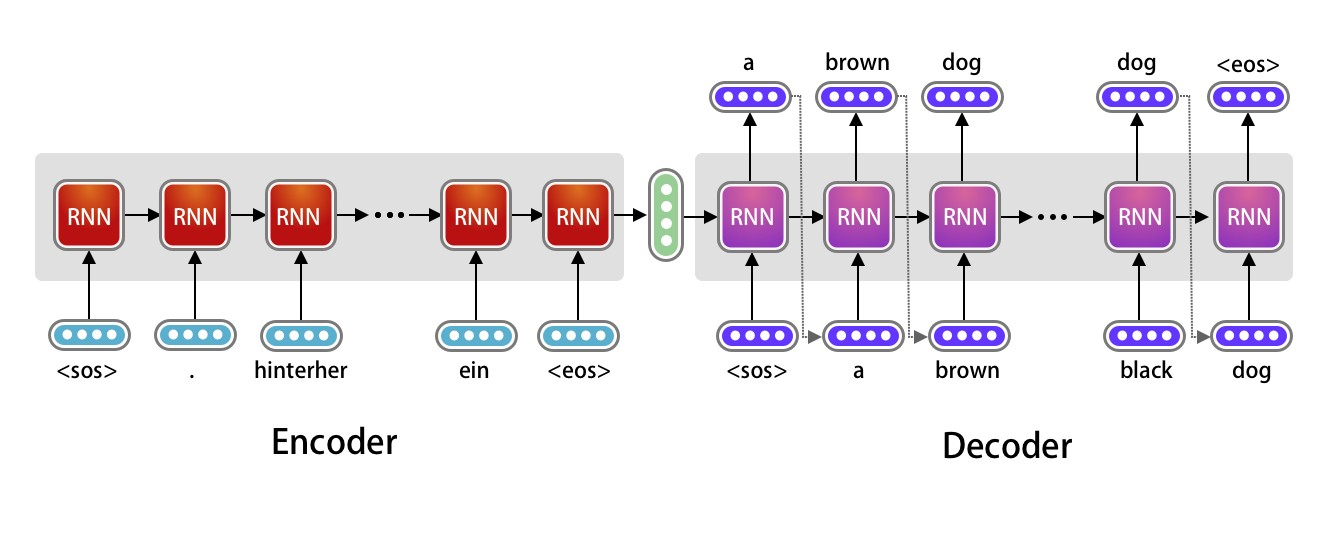
\includegraphics[width=\textwidth]{obrazky-figures/rnn}
    \caption{Encoder-Decoder Model for machine translation. Adapted from \cite{rnn}}
    \label{pic:rnn}
\end{figure}


RNNs and their variants are foundational to speech recognition in the deep learning sphere \cite{Mehrish_2023}. Nevertheless, even successful sequence-to-sequence models that leverage these RNN architectures grapple with slow training times and precise capturing of long-term dependencies remains difficult~\cite{Goodfellow-et-al-2016}.


\section{Transformer}
The introduction of the transformer architecture marked a paradigm shift in sequence-to-sequence modeling. Originally introduced by \textit{Vaswani et al. in Attention is All You Need}~\cite{vaswani2017attention}, the transformer addressed many limitations inherent in RNNs. Significantly accelerating training times, it entirely eliminated recurrence, allowing for parallelization during training. Transformers rely on the attention mechanism, described in more detail in \ref{attention-theory}, which allows the model to directly compute relationships between any position in the entire sequence, which enables better capture of long-range dependencies compared to sequential architectures like RNNs. This parallel processing capability offers a critical advantage, particularly during training. Unlike the sequential processing inherent in RNNs, transformers can compute representations for all sequence positions simultaneously, enabling training acceleration on parallel hardware. Additionally, the multi-head attention component captures relationships across different segments of the input sequence, whereas positional encodings inject information about token order to preserve the sequence’s structural integrity. This helps address the lack of inherent position representation in traditional sequence-to-sequence models.

As transformers gained prominence, they proved effective in speech recognition and other similar tasks that require processing data as sequences. They surpassed RNN-based models in performance, scalability, and efficiency. The encoder-decoder structure of the transformer, similar to the seq2seq RNN models, enables the transformer models to process and output sequences of different lengths. Given these advantages over RNN-based models, the transformer has become a foundational architecture in many tasks. It often serves as the backbone for state-of-the-art models in speech processing tasks \cite{latif2023transformersspeechprocessingsurvey}. The architecture of the original transformer is pictured in Figure \ref{pic:att}.

\begin{figure}[h!]
    \centering
    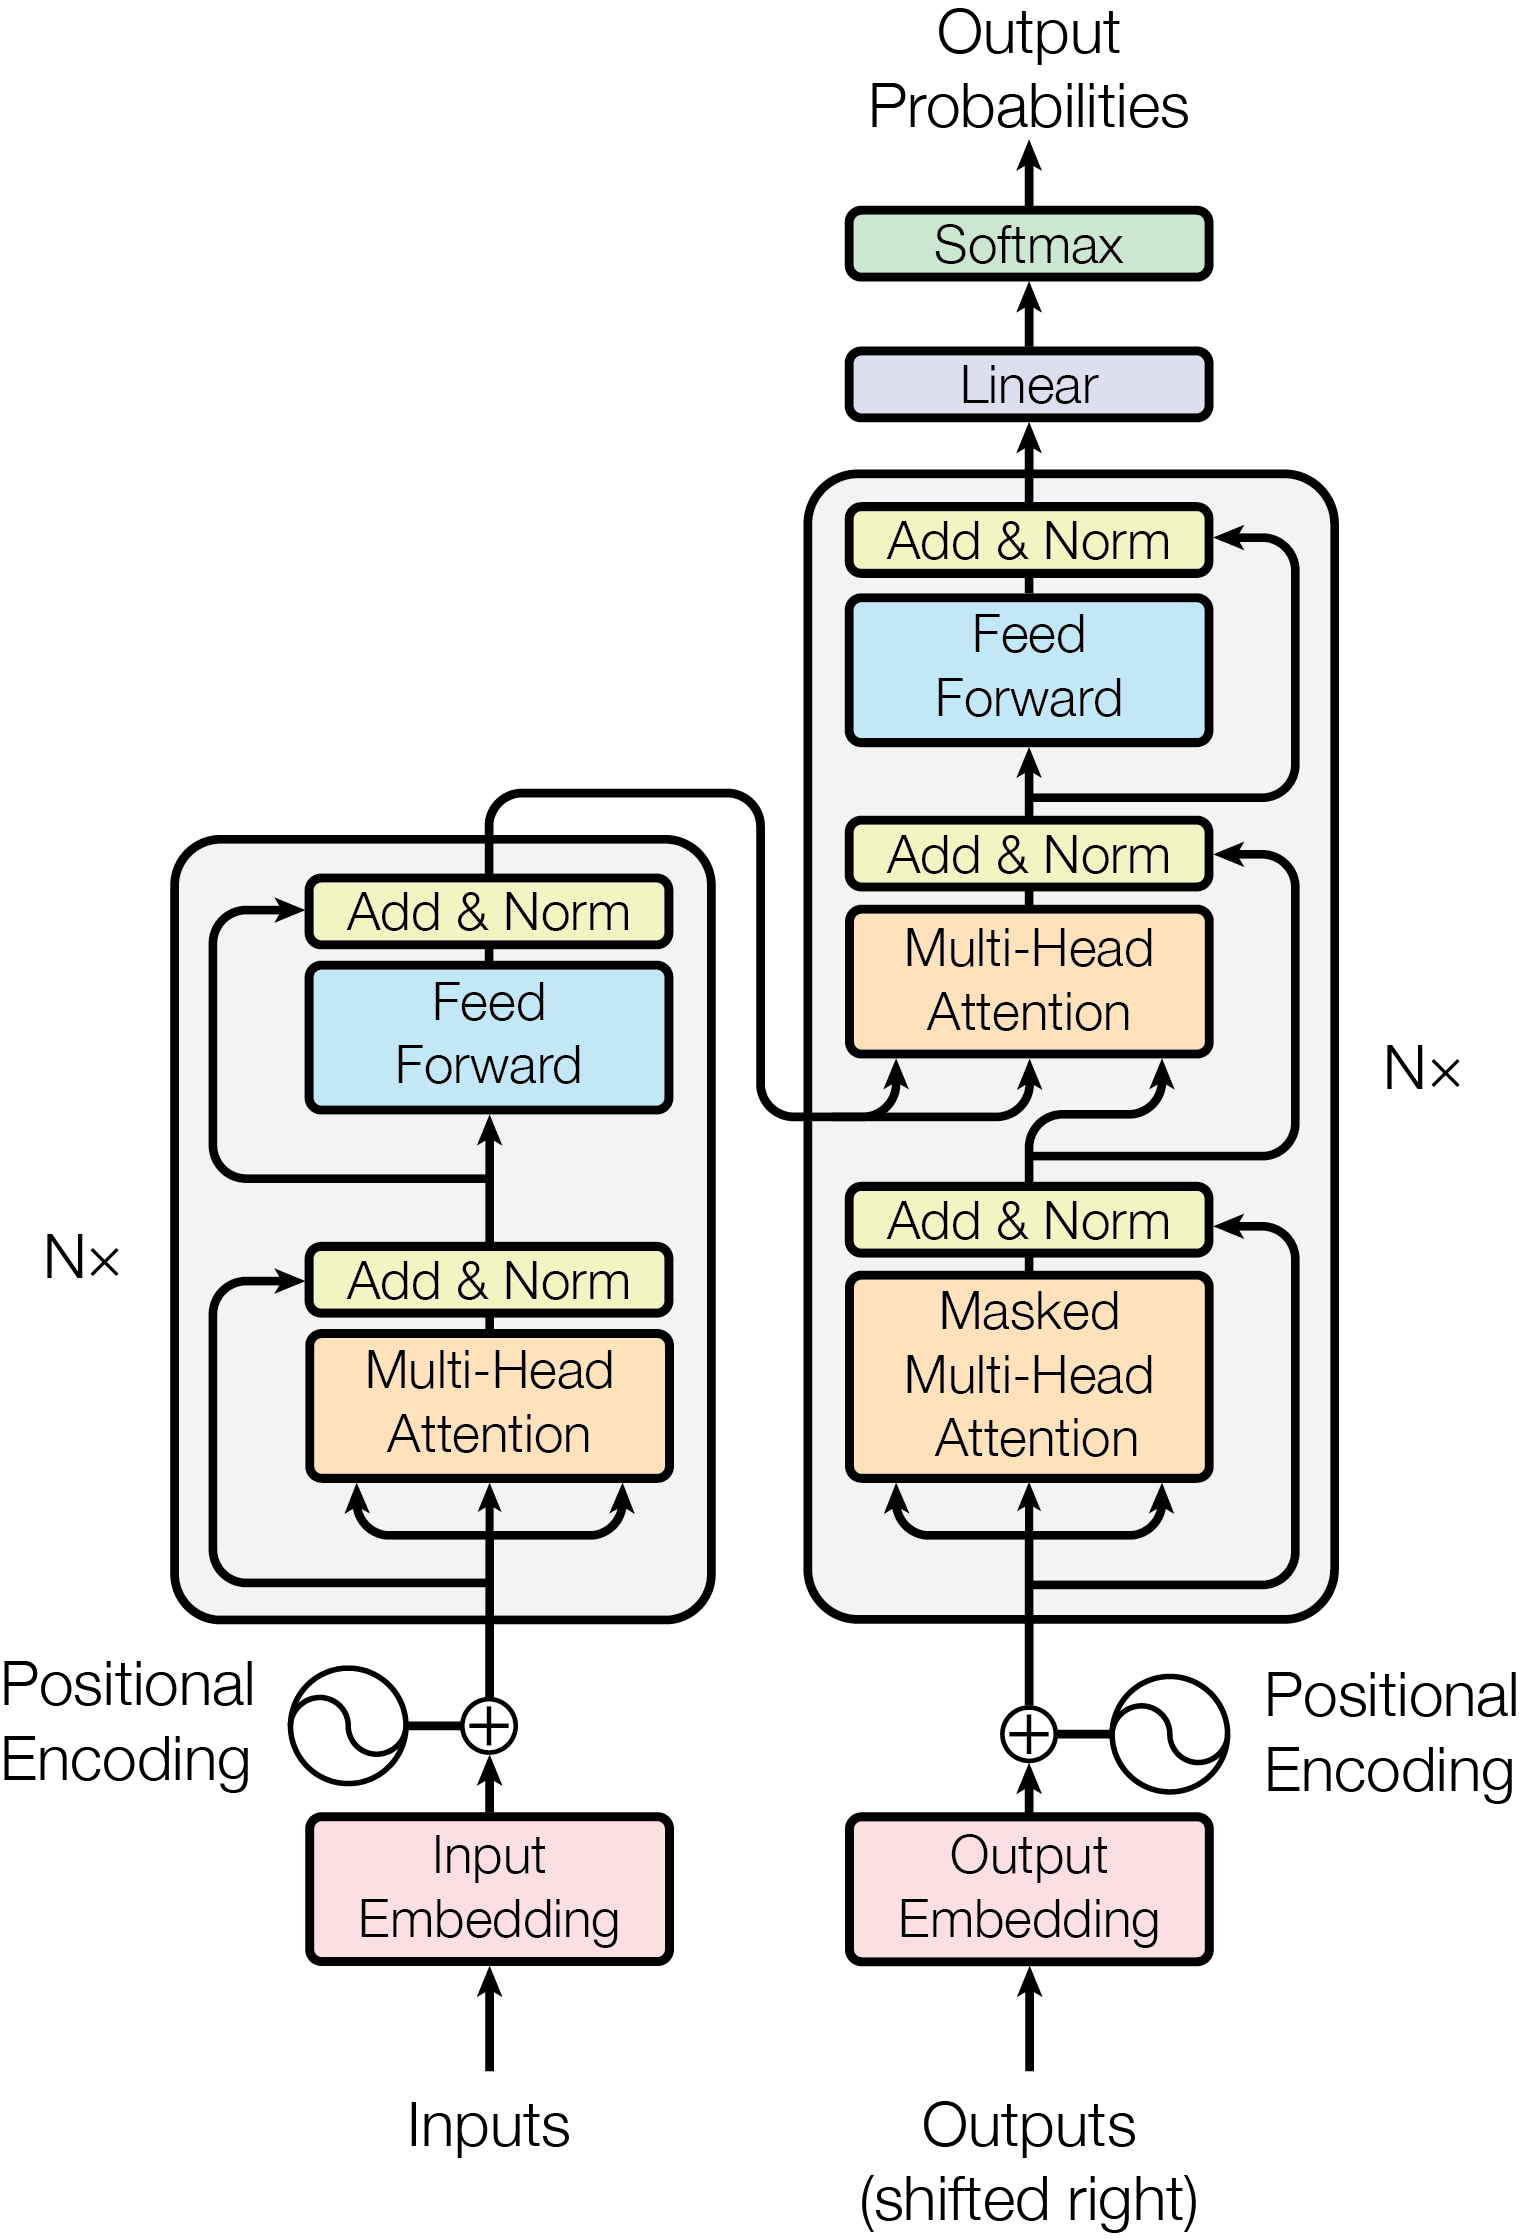
\includegraphics[width=0.6\textwidth]{obrazky-figures/att.png}
    \caption{Architecture of encoder-decoder based transformer as published in the original paper. Image taken from \cite{vaswani2017attention}.}
    \label{pic:att}
\end{figure}


\subsection{Attention mechanism} \label{attention-theory}
Attention is a method used to determine the importance of parts within a sequence. It is represented by weights assigned to each part in a sequence. In language processing, attention scores are calculated for each token on how significant they are for the currently processed token in a sequence. Models can selectively attend to different parts of the input data, assigning varying degrees of importance or weight to specific elements. Its inspiration comes from the attention of humans, where we prioritize certain stimuli or thoughts to the exclusion of others\cite{Corbetta2002}.

The first work that resembled the attention mechanism as we know it today was published in work from 1998 called \textit{A Model of Saliency-Based Visual Attention for Rapid Scene Analysis} \cite{730558}. Handcrafted features were used to create saliency maps, which guided another neural network in analyzing image patches based on importance. 

A key aspect of attention can be expressed by the following:

\begin{equation}
\sum_{i} \langle (\text{query})_i, (\text{key})_i \rangle (\text{value})_i
\end{equation}

where, the angled brackets represent dot product between \textbf{query} and \textbf{key}. 

The theoretical foundations of modern attention mechanisms can be traced to earlier architectural paradigms where a dual-network system demonstrated dynamic weight adaptation. In this framework, one network operates as a meta-learner, utilizing gradient descent to generate key-value pairs that control the weight dynamics of a second network. This second network computes answers to queries within the dynamically adjusted space \cite{hinton1987using, ha2016hypernetworks, fastweight}. The mathematical formulation of this weight-modulation mechanism was subsequently proven to be equivalent to unnormalized linear transformer architectures \cite{schlag2021linear}.
\newline

The attention mechanism was first used to solve tasks in machine translation. It used a sequence-to-sequence model with encoder-decoder architecture. \textit{Bahdanau et al.} \cite{bahdanau2014neural} identified that using fixed-length vectors created a bottleneck in the basic RNN encoder-decoder architecture. They proposed a novel approach that allowed the model to automatically search for relevant parts of a source sentence when predicting target words without requiring explicit segmentation. This approach achieved state-of-the-art results for machine translation at that time.

The idea of attention was expanded in work by \textit{Xu et al.} in 2015 \cite{pmlr-v37-xuc15}. They used an attention mechanism on images, where different regions or \textit{patches} with fixed dimensions of an input image were dynamically weighted, allowing the model to focus on relevant parts of the image as it produced each word of the description. 

The first innovation in \cite{vaswani2017attention} is called self-attention, which fundamentally transformed neural network design by allowing parallel computation of attention weights through matrix multiplications. This approach enabled more efficient sequential data processing by computing attention through dot products of query, key, and value matrices.
\newline

The attention operates through three interconnected vector components: a query vector, a key vector, and a value vector. Each vector serves a specific computational purpose in deriving the attention output. When implemented, these vectors are typically arranged into comprehensive matrices representing queries (\textbf{Q}), keys (\textbf{K}), and values (\textbf{V}). Using matrices for query, key, and value vectors enables simultaneous attention computation across multiple tokens, allowing neural networks to capture contextual relationships more efficiently. The scaled dot-product attention characteristic of transformer architectures is mathematically expressed through the formula: 

\begin{equation}
\begin{aligned}
\text{Attention}(\textbf{Q}, \textbf{K}, \textbf{V}) &= \text{Softmax}\left(\frac{\textbf{Q}\textbf{K}^T}{\sqrt{d_k}}\right)\textbf{V} \\
\textbf{Q} &= \textbf{W}_Q\textbf{X} \\
\textbf{K} &= \textbf{W}_K\textbf{X} \\
\textbf{V} &= \textbf{W}_V\textbf{X} \\
\end{aligned}
\end{equation}


where the variables: $\textbf{Q}, \textbf{K}, \textbf{V}$ representing the Query, Key, and Value matrices, respectively; $\textbf{W}_Q \in \mathbb{R}^{d_{\text{model}} \times d_q}$, $\textbf{W}_K \in \mathbb{R}^{d_{\text{model}} \times d_k}$, $\textbf{W}_V \in \mathbb{R}^{d_{\text{model}} \times d_v}$ are the projection weight matrices for Query, Key, and Value, respectively; and $\textbf{X} \in \mathbb{R}^{n \times d_{\text{model}}}$ is the input embedding matrix, where each row represents the embedding of a token in the sequence.

The dimensions involved are: $n$, the sequence length (i.e., the number of tokens in the input); $d_{\text{model}}$, the dimensionality of each token's embedding vector; and $d_q, d_k, d_v$, the dimensionalities of the Query, Key, and Value vectors, respectively.

For normalization, the scaling factor $\frac{1}{\sqrt{d_k}}$ prevents excessively small gradients in the softmax computation, which could hinder learning, particularly for long sequences. This ensures stable updates during backpropagation.


A computation diagram of the scaled dot-product attention is shown in Figure \ref{fig:subfig-a}.
\newline


\begin{figure}[h]
    \centering
    \begin{subfigure}[b]{0.45\textwidth}
        \centering
        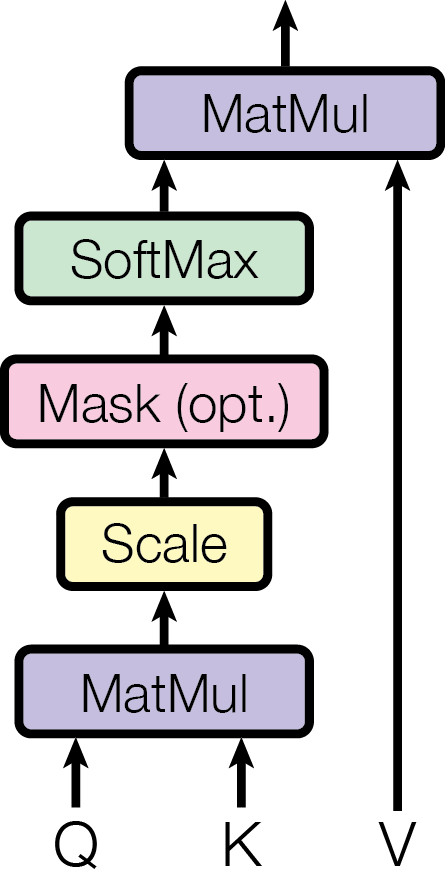
\includegraphics[width=0.6\linewidth]{obrazky-figures/scaleddotattn.png}
        \caption{Scaled dot-product attention.}
        \label{fig:subfig-a}
    \end{subfigure}
    \hfill
    \begin{subfigure}[b]{0.45\textwidth}
        \centering
        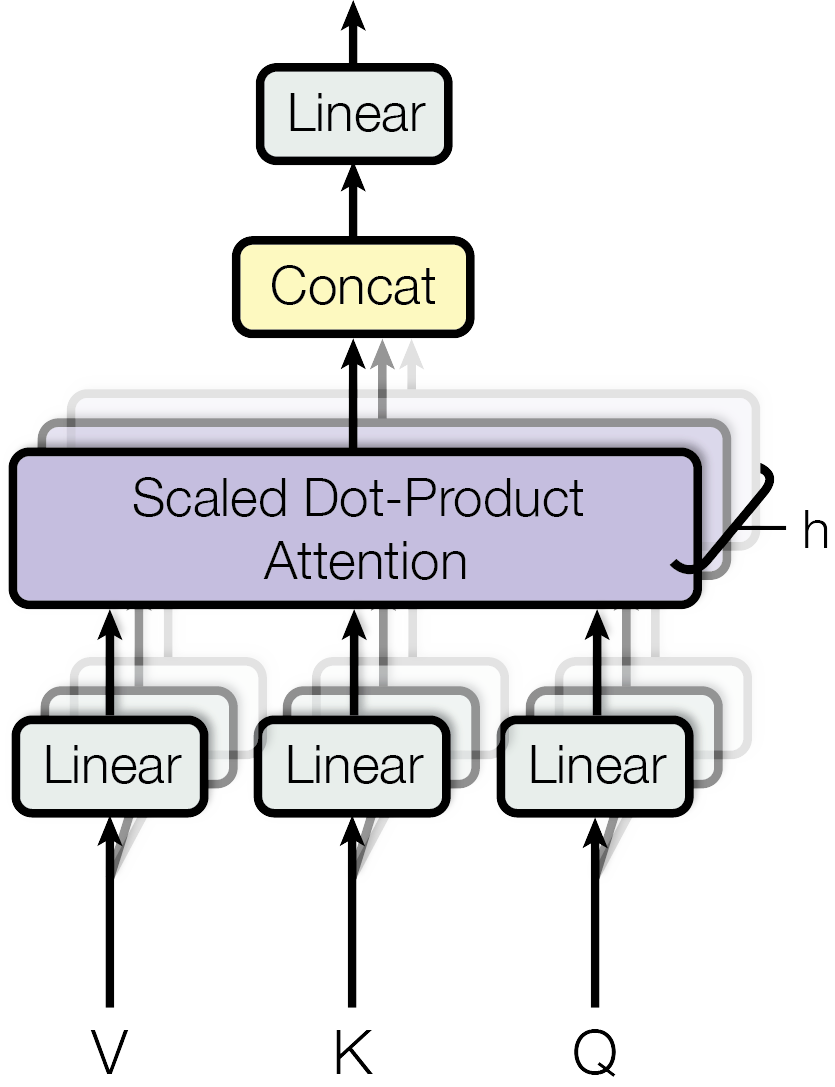
\includegraphics[width=0.92\linewidth]{obrazky-figures/multihead.png}
        \caption{Multi-head attention block.}
        \label{fig:subfig-b}
    \end{subfigure}
    \caption{Attention Mechanisms in Transformers: Scaled Dot-Product and Multi-Head Attention. $\textbf{Q}$, $\textbf{K}$ and $\textbf{V}$ denotes the query, key and value inputs. Figures taken from \cite{vaswani2017attention}.}
    \label{fig:main-figure}
\end{figure}


The second innovation that was introduced is a mechanism called Multi-head attention, which improves the model's ability to capture various relationships within the data. In the multi-head attention, input queries, keys, and values are segmented into $h$ parallel processing paths, with each head $h_i$ possessing unique projection matrices $\textbf{Q}_i$, $\textbf{K}_i$ and $\textbf{V}_i$. Instead of using a single attention function with $d_{\text{model}}$ dimensional keys, values, and queries, Multi-head attention projects the queries, keys, and values into different subspaces, with dimensions $\text{d}_k$, $\text{d}_k$, and $\text{d}_v$, respectively. Attention is then computed in parallel for each projection, producing outputs that are concatenated and projected to generate the final result. This approach enables the model to attend to multiple aspects of the input simultaneously, as illustrated in Figure \ref{fig:subfig-b}.

Mutli-head attention is represented by following formula:

\begin{equation}
\begin{aligned}
\text{MultiHead}(\textbf{Q}, \textbf{K}, \textbf{V}) &= \text{Concat}(\text{head}_1, \ldots, \text{head}_h)W^O \\
\text{where } \text{head}_i &= \text{Attention}(\textbf{Q}W^Q_i, \textbf{K}W^K_i, \textbf{V}W^V_i)
\end{aligned}
\end{equation}

% In their paper they use d_k and d_v without d_q
where the projections are parameter matrices $W^Q_i \in \mathbb{R}^{d_{\text{model}} \times d_k}$, $W^K_i \in \mathbb{R}^{d_{\text{model}} \times d_k}$, $W^V_i \in \mathbb{R}^{d_{\text{model}} \times d_v}$ and $W^O \in \mathbb{R}^{hd_v \times d_{\text{model}}}$. Dimensions of $d_k$, and $d_v$ are $d_{\text{model}}/h$. The $W^O$ matrix serves to linearly project the concatenated multi-head attention outputs back to the original model dimension $d_{\text{model}}$, allowing the multi-head attention to integrate and transform the parallel attention computations into a single, coherent matrix representation.
\newline

There are small differences in the encoder and decoder attention. In the encoder, self-attention, as described earlier, allows each position in the input sequence to attend to all other positions. This is particularly important in machine translation, where variations in word order and syntax between languages require the model to capture long-range dependencies across the entire input sequence.

The decoder's attention mechanism differs depending on its role. When used for autoregressive sequence generation it employs masked attention, also called causal attention. This is fundamentally important for autoregression because it prevents positions from seeing future tokens in the sequence during training and generation. By blocking attention to subsequent positions, it ensures causality – the current prediction depends only on past information. This masking mechanism in attention is done by matrix $M$ to zero out attention scores for future tokens:

\begin{equation}
    M_{ij} =
\begin{cases} 
0 & \text{if } i < j, \\
-\infty & \text{if } i \geq j.
\end{cases}
\end{equation}

Matrix $M$ is then added to the calculation of attention:

\begin{equation}
\text{Masked Attention}(\textbf{Q}, \textbf{K}, \textbf{V}) = \text{Softmax}\left(\frac{\textbf{Q}\textbf{K}^T + M}{\sqrt{d_k}}\right)\textbf{V}
\label{masked_att}
\end{equation}

With this small difference, the decoder maintains an autoregressive property that is vital for generating sequences in a step-by-step manner.


In addition to this masked self-attention mechanism, each decoder layer also incorporates a cross-attention mechanism. This is a link that allows the decoder to incorporate information from the encoder. In this cross-attention sub-layer, the \textbf{query} vectors (\textbf{Q}) originate from the output of the preceding decoder sub-layer. However, the \textbf{key} (\textbf{K}) and \textbf{value} (\textbf{V}) vectors are derived directly from the encoder’s contextual representations. The computation uses the same scaled dot-product attention formula:
\begin{equation}
\text{Cross-Attention}(\textbf{Q}_{\text{dec}}, \textbf{K}_{\text{enc}}, \textbf{V}_{\text{enc}}) = \text{Softmax}\left(\frac{\textbf{Q}_{\text{dec}}\textbf{K}_{\text{enc}}^T}{\sqrt{d_k}}\right)\textbf{V}_{\text{enc}}
\label{cross_att}
\end{equation}

This mechanism enables the decoder, at each step, to dynamically focus on the most relevant parts of the encoded input sequence. Unlike self-attention, cross-attention computes relationships between two different sequences: the decoder's intermediate representations and the encoder's final output.
\newline



\begin{figure}[h!]
    \begin{subfigure}[b]{0.58\textwidth}
        \centering
        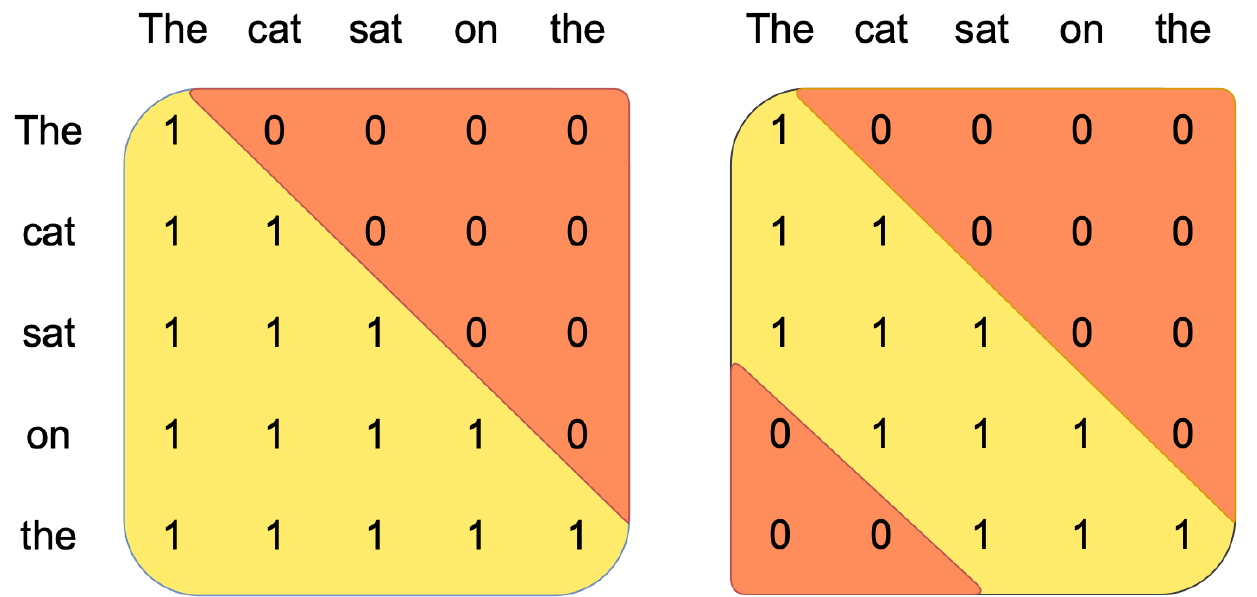
\includegraphics[width=1\linewidth]{obrazky-figures/slidingwatt.png}
        \caption{Masked attention and sliding window attention. Figure taken from \cite{jiang2023mistral}.}
        \label{att:sliding}
    \end{subfigure}
    \begin{subfigure}[b]{0.38\textwidth}
        \centering
        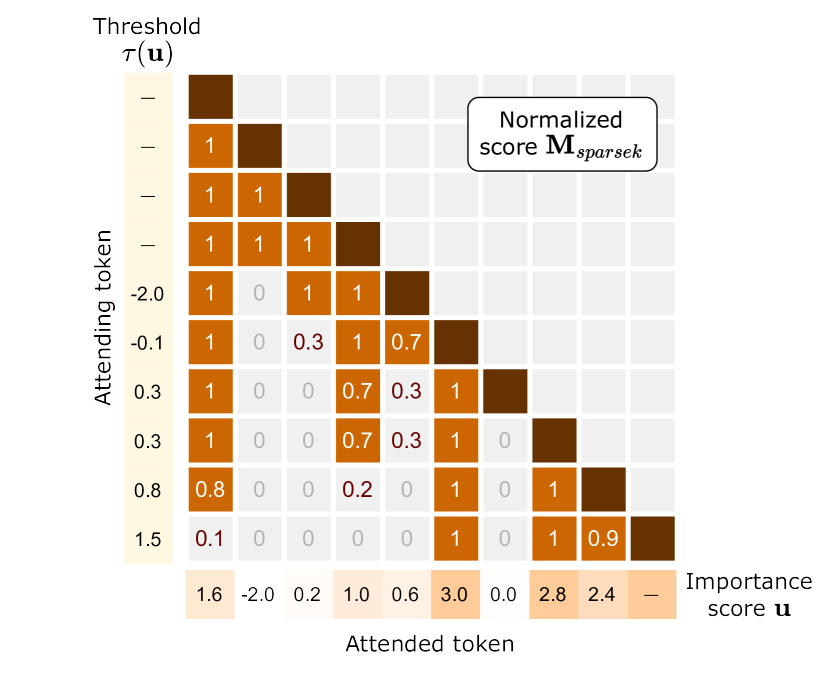
\includegraphics[width=1\linewidth]{obrazky-figures/sparse.png}
        \caption{Sparse attention. Figure taken from \cite{lou2024sparser}.}
        \label{att:sparse}
    \end{subfigure}
    \caption{Different attention mechanisms used in transformer models.}
    \label{att:main-figure}
\end{figure}


\subsection{Improvements in Attention mechanism}
Different attention mechanisms have been created to explore more computationally efficient and contextually nuanced alternatives. One strategy called sliding window attention was introduced together with the family of language models from the company \textit{Mistral AI}\footnote{https://mistral.ai/}. It restricts attention computation to only the last $n$ elements in a sequence, which enables more efficient processing of long-range dependencies in sequence \cite{jiang2023mistral}. This is shown in Figure \ref{att:sliding}. Sparse attention also tries to address the efficiency of computational resources by reducing the number of attention connections between tokens \cite{zaheer2020big}. This approach uses intelligent sparsity patterns to remove some connections. Sparse attention is depicted in Figure \ref{att:sparse}.


Similar to attention mechanism improvements, more efficient techniques have been introduced to improve multi-head attention. Attention mechanism innovations have further improved computational efficiency and model performance through techniques like multi-query attention (MQA) and grouped-query attention (GQA). Multi-query attention modifies the multi-head attention approach by sharing key and value projection matrices across all heads, reducing computational complexity together with computational resources. This, however, comes with slightly lower accuracy scores for models \cite{mqa}. Grouped-query attention \cite{kitaev2020reformer} represents a better compromise between traditional multi-head and multi-query attention, where a subset of heads share key and value projections, which offers a balanced approach to reducing computational overhead. The grouped-query attention can be mathematically represented as:


\begin{equation}
\begin{aligned}
\text{GroupedQueryAttention}(\textbf{Q}, \textbf{K}, \textbf{V}) &= \text{Concat}(\text{group}_1, \ldots, \text{group}_g)W^O \\
\text{where } \text{group}_j &= \text{Attention}\left(\textbf{Q}W^Q_j, \underbrace{\textbf{K}W^K_g, \textbf{V}W^V_g}_{\text{shared within group}}\right)
\end{aligned}
\end{equation}

where, $g$ represents the number of groups, with each group sharing key and value projections, allowing for a flexible trade-off between computational efficiency and model robustness. It was shown that this improves the model performance while maintaining the same model's ability.



\subsection{Embeddings}
Embeddings are a foundational component within transformer architectures, responsible for converting discrete input tokens into dense, continuous vector representations. This initial transformation is crucial because simpler methods, like one-hot encoding, while uniquely identifying tokens, produce sparse, high-dimensional vectors that fail to capture inherent semantic or syntactic relationships between them \cite{42543}. These learned embeddings encode such information so that relationships between tokens (like similarity, analogy, or contextual relatedness) are often captured by the geometric relationships (e.g., distance, orientation) between their corresponding vectors in the embedding space. The dimensionality of these vectors is a key hyperparameter, commonly set between 256 and 4096, influencing the model's capacity and computational cost \cite{bai2023qwen, touvron2023llama}. 


Static word embedding methods, including Word2Vec \cite{word2vec}, GloVe \cite{pennington-etal-2014-glove}, and FastText \cite{fasttext}, generate a single vector representation for each token. This means a word will have the same embedding regardless of its surrounding words or the sense it's used in. While useful for many applications, this static nature limits their ability to model how word meanings shift and adapt across different contexts.


Contextual embeddings, introduced with transformer architecture, address this limitation by generating context-dependent representations. These embeddings are better suited since their meaning is dependent on its surrounding data. During the training process, both embeddings and model parameters collectively form the set of parameters of the model.

The embedding layer is represented as a matrix $\mathbf{E} \in \mathbb{R}^{|V| \times d}$, where $|V|$ is the vocabulary size and $d$ is the embedding dimensionality. Each row of $\mathbf{E}$ corresponds to a vector representation of a token in the vocabulary.
Given a token $x_i$ with index $i$ in the vocabulary, its embedding is computed as:

\begin{equation}
\text{Embedding}(x_i) = \mathbf{E}[x_i]
\end{equation}



\subsection{Positional Encodings}
Transformers process input sequences using parallel computation and self-attention, mechanisms that do not inherently encode the position of tokens within the sequence. Positional encodings are crucial components that inject information about the relative or absolute positions of tokens in the sequence. These encodings enable the model to understand and utilize sequential order in its computations.

The original transformer paper introduced sinusoidal positional encodings \cite{vaswani2017attention}, which use sine and cosine functions of different frequencies to represent positions. For position $pos$ and dimension $i$ in a $d$-dimensional embedding space, the encodings are computed as:


\begin{equation}
\begin{aligned}
PE_{(pos,2i)} = \sin\left(\frac{pos}{10000^{2i/d_{\text{model}}}}\right) \\
PE_{(pos,2i+1)} = \cos\left(\frac{pos}{10000^{2i/d_{\text{model}}}}\right)
\end{aligned}
\end{equation}
where $pos$ is the position in the sequence, and $i$ is the dimension index. This formulation handles sequences of arbitrary length. 


An alternative approach is learned positional embeddings \cite{devlin2019bertpretrainingdeepbidirectional}, where the position vectors are treated as model parameters and learned during training. It is simpler to implement; however, learned embeddings are limited to a maximum sequence length defined during training and do not inherently generalize to longer sequences.

Another approach called Attention with Linear Biases (ALiBi) \cite{press2022trainshorttestlong} offers a position encoding method that allows models to extrapolate to sequence lengths not seen during training by adding a position-dependent scalar bias to attention scores. The key strength of ALiBi lies in its ability to allow models trained on shorter sequences to generalize to much longer sequences because the bias term is independent of sequence length.


The positional encoding is added to or combined with the token embeddings before being processed by the transformer layers:
\begin{equation}
\text{Input} = \text{Embedding}(x_i) + \text{PositionalEncoding}(pos_i)
\end{equation}

More recently, Rotary Positional Embedding (RoPE) \cite{su2023roformerenhancedtransformerrotary} has gained prominence by offering a fundamentally different approach. Instead of adding positional vectors to embeddings or biasing attention scores, RoPE encodes positional information by rotating the query (\textbf{Q}) and key (\textbf{K}) vectors based on their absolute positions within the attention mechanism itself. It takes advantage of geometric properties, applying position-dependent rotation matrices to pairs of dimensions in the \textbf{Q} and \textbf{K} vectors before computing the dot product.

The core innovation of RoPE lies in how this rotation affects the query-key interaction. The rotation is designed such that the dot product between the rotated query vector at position $m$ and the rotated key vector at position $n$ depends only on the original query and key vectors and their relative position $m-n$. RoPE's advantages include inherently encoding relative positions and maintaining sequence order via geometric rotations within the attention mechanism. This yields better performance and generalization to longer sequences than additive methods.


\subsection{Tokenization}
End-to-end systems process input data as raw inputs, meaning speech signals are directly captured from a microphone or text strings for natural language processing. The input sentence is split into discrete parts, called tokens. This step enables transformer models to handle the input data by converting it into a sequence of manageable, discrete units. This preprocessing step directly impacts model performance and efficiency \cite{Rust_2021}.

World-level tokenization is the simplest approach. It splits text on whitespace and punctuation. It is intuitive but struggles with out-of-vocabulary words and requires a large vocabulary to cover most words in a language.

Character-level tokenization represents text as individual characters, which solves out-of-vocabulary problems. Using characters as tokens also means that vocabulary will be minimal. However, this approach generates longer sequences and fails to capture meaningful semantic units.

Byte-Pair Encoding (BPE) \cite{bpe_sennrich-etal-2016-neural} is the dominant tokenization method in modern transformer architectures. BPE makes a balance between word and character-level approaches by learning subword units from the training data. The algorithm iteratively merges the most frequent pair of consecutive bytes or characters to create a new token, thus creating a vocabulary of optimal subword units. The training process is formally described at \ref{ref:bpe}.


\begin{algorithm}
\caption{Byte-Pair Encoding (BPE) algorithm}\label{ref:bpe}
\begin{algorithmic}[1]
\Require Training corpus $C$, target vocabulary size $V$
\State Initialize:
\State \quad $\text{Vocab} \gets \text{set of individual characters in } C$
\State \quad Split each word in $C$ into character sequences
\While{$|\text{Vocab}| < V$}
    \State $(x, y) \gets \arg\max_{(a, b) \in \text{pairs}(C)} \text{count}((a, b))$
    \State Add merged token $xy$ to $\text{Vocab}$
    \State Replace all occurrences of $(x, y)$ with $xy$ in $C$
\EndWhile
\State \Return $\text{Vocab}$
\end{algorithmic}
\end{algorithm}

Other variants include WordPiece \cite{wordpiece} and Unigram \cite{unigram}. These approaches rely on probabilistic approaches to token merging. Similar to BPE, SentencePiece \cite{Kudo_2018} processes text as unicode sequences and applies this algorithm language-agnostically. This ensures consistent tokenization across different scripts. Unigram is used in conjunction with SentencePiece.

Tokenizers employ several special tokens that provide context and structural guidance to the model. These special tokens serve specific roles during training and model inference. They mark the beginning and end of sequences, indicate padding, separate different input components, or act as special instructions in order for the model to understand the structure of the input data. Commonly, these special tokens are represented using formats like \texttt{[PAD]}, \texttt{<EOS>}, and \texttt{[MASK]}, respectively representing sequence padding, end-of-sequence marking, and enabling masked language modeling during pre-training.

The tokenization method and vocabulary size are fundamental design decisions in transformer architectures. Vocabulary size impacts the model's computational performance, where larger vocabularies reduce sequence lengths but increase the parameter count in the following embedding layers. Meanwhile, smaller vocabularies result in longer sequences with fewer parameters.


\subsection{Encoder}
Encoder is the first part of the transformer that processes the input sequence and produces a continuous representation or embeddings of the input sequence. Visual representation of an encoder part of a transformer model is shown in figure \ref{pic:att}. The encoder captures the context of each token with respect to the entire sequence.

Transformer models often employ more than one encoder layer. In the original architecture, one encoder layer comprises of two sub-modules: a multi-head self-attention mechanism and a fully connected feed-forward network. Additionally, it incorporates residual connections around each sub-module, which are then followed by a normalization layer. In the original paper \cite{vaswani2017attention}, the normalization layer was applied after the attention and feed-forward layers. Current transformer architectures use a normalization layer before attention and a feed-forward layer. This small change has been shown to make the training of transformer models more stable \cite{xiong2020layernormalizationtransformerarchitecture}. For the normalization layer, LayerNorm was used, but in recent transformer models, it is more common to use  Root Mean Square Layer Normalization (RMSNorm) instead. It is more computationally efficient and often shows comparable or slightly better performance \cite{zhang2019rootmeansquarelayer}. 


Within each encoder layer, multi-head self-attention is utilized. This allows the encoder to process the input sequence by relating each token to every other token, effectively capturing the contextual information from the entire sequence in parallel across different representation subspaces ('heads').



\subsection{Decoder}
Decoder is the second part of the transformer. It is responsible for generating the output sequence based on the encoder's representations. As shown in figure \ref{pic:att}, the decoder processes the encoder's output and generates tokens sequentially.

Each decoder layer typically comprises three main sub-layers, along with residual connections and layer normalization, similar in structure to the encoder layers but with distinct functions. The first sub-layer is a masked multi-head self-attention mechanism. This masking ensures the autoregressive property, preventing the model from seeing future tokens during generation. The second sub-layer is the multi-head cross-attention mechanism. This is where the decoder interacts with the encoder's output: the query vectors (\textbf{Q}) originate from the decoder's state, while the key (\textbf{K}) and value (\textbf{V}) vectors are taken directly from the final representation sequence produced by the encoder. This allows the decoder, at each step, to focus on the most relevant parts of the input sequence's representation when predicting the next output token. The third sub-layer is a standard position-wise feed-forward network. The decoder operates autoregressively, beginning with a start token and generating tokens sequentially, using previously generated outputs and the context derived from the encoder via cross-attention, until an end token is produced.

One layer comprises of three sub-modules: masked attention \ref{masked_att}, cross attention, and feed-forward network. Cross attention mixes data from the encoder and decoder part; queries originate from the results of the preceding decoder sub-module, while keys and values stem from the outputs of the encoder. This aligns the encoder's input with the decoder's input. 

Finally, within the decoder architecture specifically configured for ASR, a linear layer followed by a softmax function acts as the output layer. This linear layer projects the decoder's final hidden state representation into a vector whose size matches the target vocabulary. It produces raw logit scores for each potential token. The subsequent softmax layer then transforms these logits into a probability distribution over the entire vocabulary, indicating the likelihood of each token being the next element in the generated transcription. During inference, the model selects the next token based on these probabilities to build the output text sequence word by word (or token by token).
The chosen token is then fed back together with the previous input as a new input for the decoder. Decoding process continues until the model produces a token that signals end of generation for the model. Because of this auto-regressive process, it is sequential and time-consuming compared to the encoder.
\newline

\chapter{End-to-End Architectures for Automatic Speech Recognition}\label{chap_e2e_archs}

Building upon the foundational concepts of the transformer architecture discussed in Chapter \ref{chap_theory}, this chapter delves into specific end-to-end architectures that have revolutionized the field of Automatic Speech Recognition (ASR). These architectures aim to directly map an input audio signal, either in its raw form or as processed features, to an output sequence of text.

\section{Introduction to End-to-End ASR}

Traditional ASR systems often involved a complex pipeline of separate modules for acoustic feature extraction, acoustic modeling, and language modeling. These modular systems were often difficult to optimize as a whole. In contrast, end-to-end ASR architectures simplify this process by learning a direct mapping from the input audio to the output text sequence using a single neural network \cite{graves2012sequence}. This paradigm shift has been enabled by advances in deep learning, particularly sequence-to-sequence models capable of handling variable-length inputs and outputs. The goal of end-to-end ASR is to train a single model that can learn all the necessary components, from extracting relevant acoustic features to generating grammatically correct and semantically meaningful transcriptions.

The three most popular end-to-end architectures dominate ASR~\cite{Li_2022, KHEDDAR2024102422}. The approaches are Connectionist Temporal Classification (CTC) \cite{graves2006connectionist, graves2014towards}, Attention-based Encoder-Decoder (AED) models \cite{chorowski2015attentionbased, Chan_2016}, and the Recurrent Neural Network Transducer (RNN-T) \cite{graves2012sequence}. These architectures differ fundamentally in how they align the audio input with the text output and generate the final sequence, as illustrated in Figure \ref{fig:e2e_architectures}. Each architecture presents distinct advantages and challenges, which will be discussed in the following sections.

Regardless of the specific end-to-end architecture, the ultimate goal during inference is to decode the input audio into the most probable text sequence. This decoding process typically involves strategies such as greedy search, which rapidly selects the most likely output token at each step based on the model's probabilities. However, to achieve higher accuracy, beam search is more commonly employed. Beam search explores a limited set of the most promising candidate transcriptions simultaneously by keeping track of a "beam" of hypotheses, offering a better approximation of the optimal sequence, although with increased computational demand.

\begin{figure}[h!]
    \centering
    \begin{subfigure}[b]{0.22\textwidth}
        \centering
        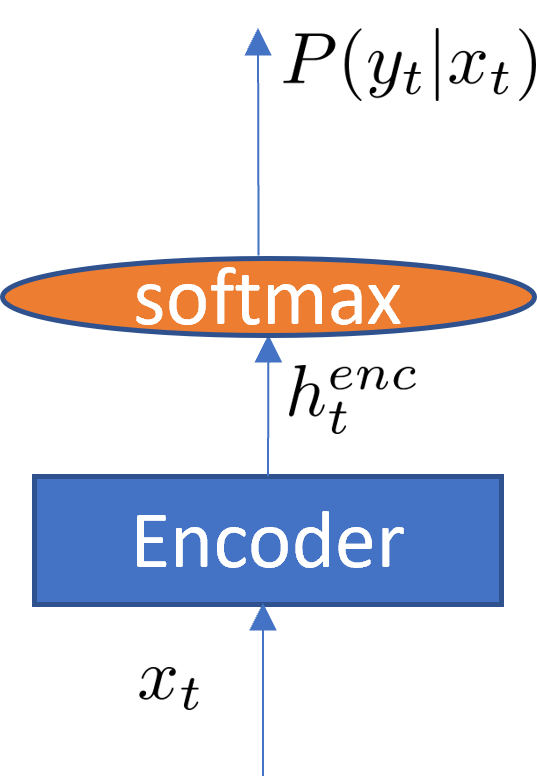
\includegraphics[width=\linewidth]{obrazky-figures/archs/CTC.png}
        \caption{CTC Architecture}
        \label{fig:ctc_arch}
    \end{subfigure}
    \hfill
    \begin{subfigure}[b]{0.32\textwidth} 
        \centering
        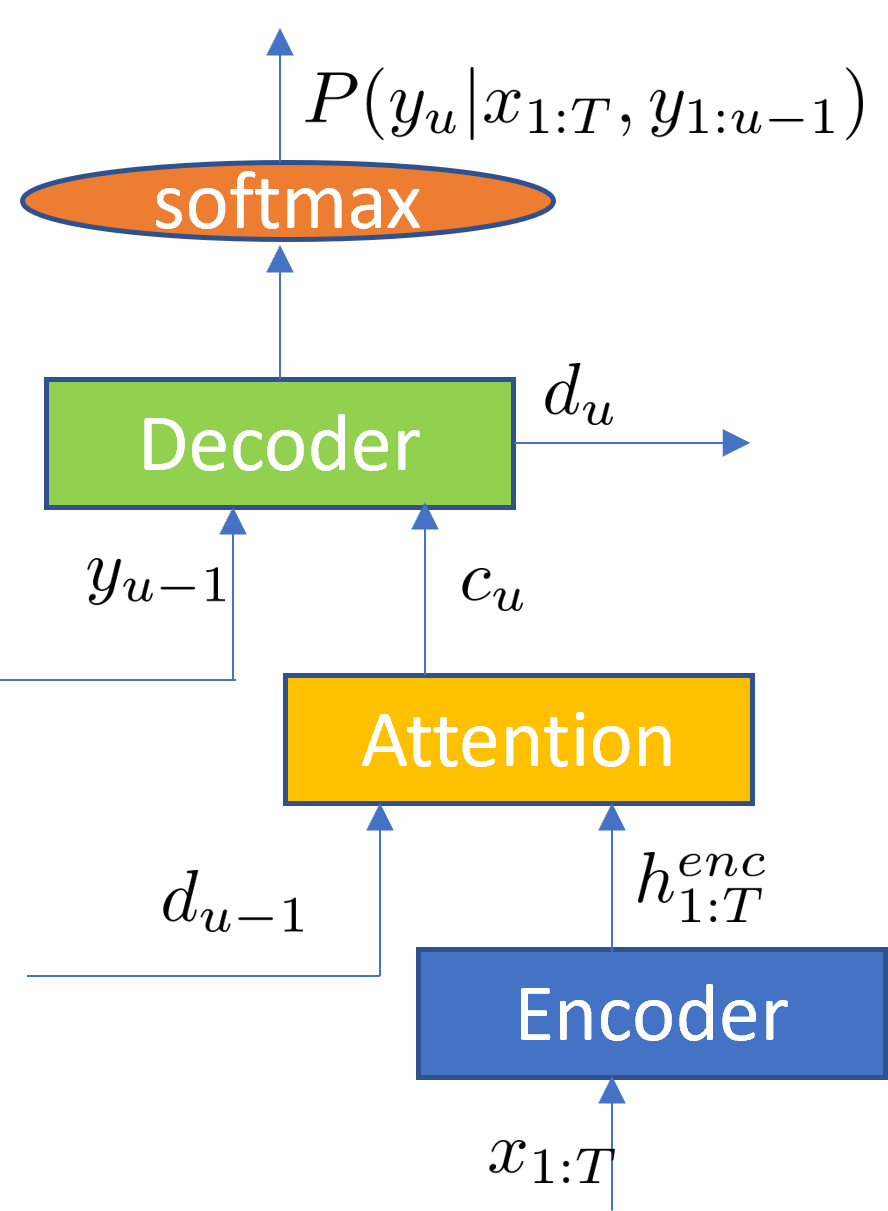
\includegraphics[width=\linewidth]{obrazky-figures/archs/AED.png}
        \caption{AED Architecture}
        \label{fig:aed_arch}
    \end{subfigure}
    \hfill
    \begin{subfigure}[b]{0.38\textwidth} 
        \centering
        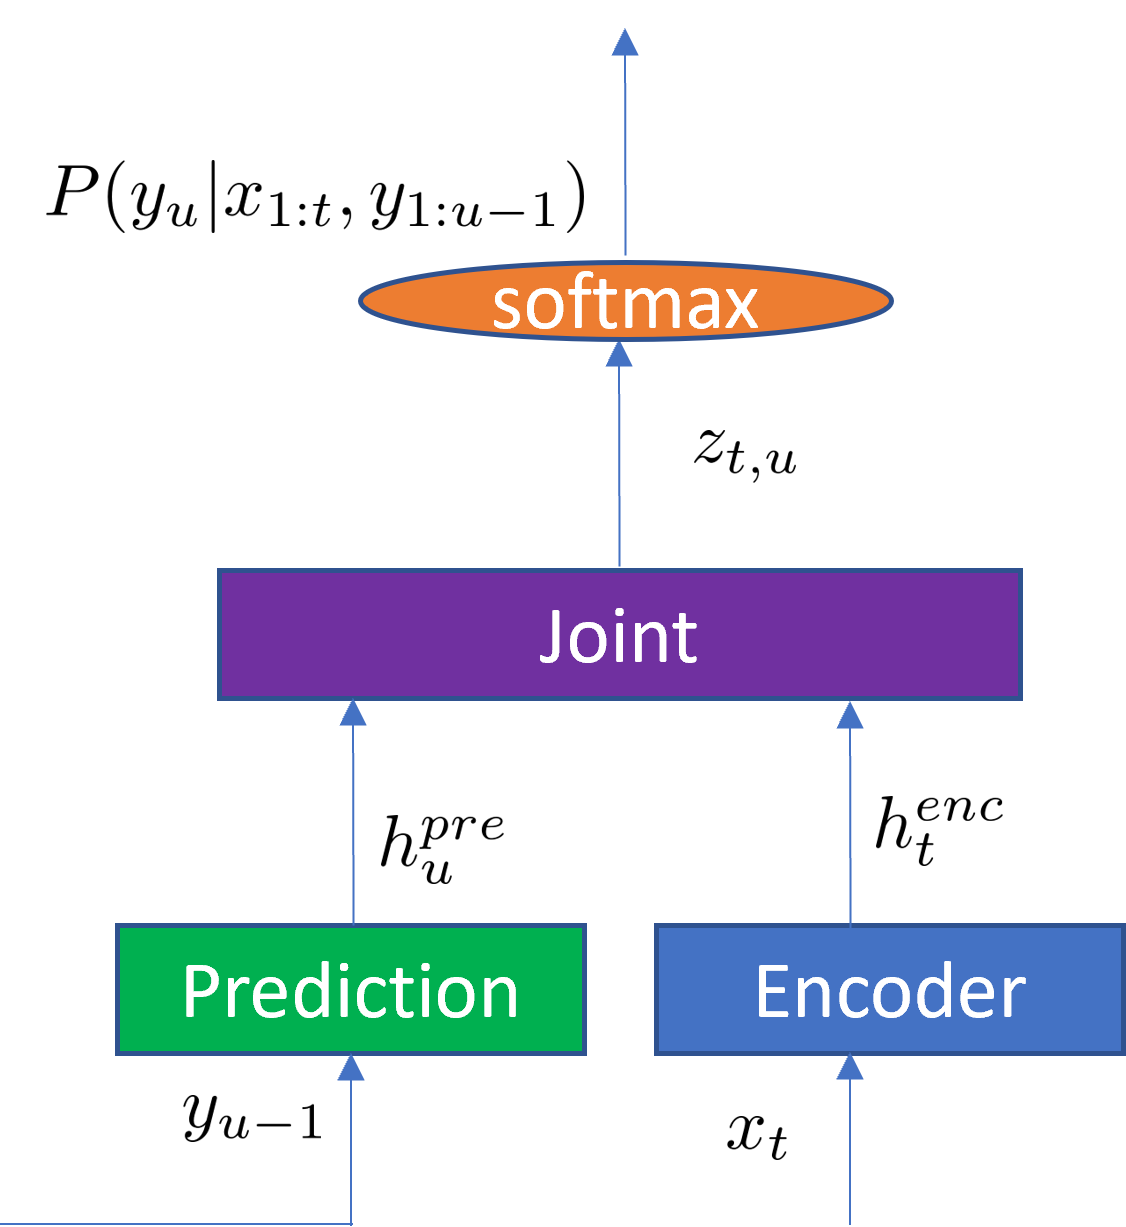
\includegraphics[width=\linewidth]{obrazky-figures/archs/RNNT.png}
        \caption{RNN-T Architecture}
        \label{fig:rnnt_arch}
    \end{subfigure}
    \caption{Diagrams of the three most common End-to-End ASR architectures: (a) Connectionist Temporal Classification (CTC), (b) Attention-based Encoder-Decoder (AED), and (c) Recurrent Neural Network Transducer (RNN-T). These illustrate their core components and information flow. Adapted from \cite{Li_2022}.}
    \label{fig:e2e_architectures}
\end{figure}


\section{Connectionist Temporal Classification (CTC)}\label{ctc_theory}

Connectionist Temporal Classification (CTC) \cite{graves2006connectionist} is an end-to-end architecture primarily used for sequence labeling tasks, including ASR. It is characterized by its encoder-only structure, where the input audio is processed by an encoder to produce a sequence of frame-level predictions.

\subsection{Architecture and Loss Function}

The CTC architecture consists of an acoustic encoder that takes the input audio features and transforms them into a sequence of higher-level representations. A linear layer followed by a softmax activation is then applied to each time step of the encoder's output, producing a probability distribution over the target vocabulary plus an additional 'blank' token. This special token serves as a hard boundary between groups of characters and also makes it possible to filter out duplicate characters.

The CTC loss function is designed to train the model without requiring explicit frame-level alignments between the audio and the text. For a given audio input and its corresponding transcription, there can be multiple possible frame-level label sequences (paths) that are consistent with the transcription. A path is considered consistent if it can be reduced to the transcription by first removing consecutive repeated labels and then removing all blank tokens. The CTC loss is the negative logarithm of the sum of probabilities of all such consistent paths.

Mathematically, let $X = (x_1, x_2, ..., x_T)$ be the input audio sequence of length $T$, and $Y = (y_1, y_2, ..., y_U)$ be the target transcription of length $U$. The model outputs a probability distribution $p(a_t | X)$ over the vocabulary $\mathcal{V} \cup \{\langle blank \rangle\}$ at each time step $t$, where $a_t$ is a label from the vocabulary or the blank token. The probability of a path $\pi = (\pi_1, \pi_2, ..., \pi_T)$, where each $\pi_t \in \mathcal{V} \cup \{\langle blank \rangle\}$, is given by $p(\pi | X) = \prod_{t=1}^{T} p(\pi_t | X)$. The CTC loss for a single input-output pair $(X, Y)$ is then:

\begin{equation}
\mathcal{L}_{CTC}(X, Y) = -\log \sum_{\pi \in \mathcal{B}(Y)} p(\pi | X)
\end{equation}

where $\mathcal{B}(Y)$ is the set of all paths $\pi$ that, after removing consecutive repeated labels and then all blank tokens, result in the transcription $Y$. The summation over all possible paths is computed using a dynamic programming algorithm based on the forward-backward algorithm.


\subsection{Characteristics}

CTC is the first E2E architecture widely used in ASR~\cite{hannun2014deep, Miao_2015, soltau2017neural, Das_2019}. CTC is known for its non-autoregressive nature, as the prediction at each time step is independent of other time steps given the input. This allows for fast decoding. However, a key limitation of CTC is the assumption of conditional independence between the output labels, which restricts its ability to model complex language structures.

\section{RNN Transducer (RNN-T)}

The RNN Transducer (RNN-T) \cite{graves2012sequence} is another end-to-end architecture designed to address some of the limitations of CTC, particularly the conditional independence assumption. RNN-T is an encoder-decoder architecture with a joiner network that learns to align the input audio with the output text in a monotonic fashion. It is important to note that when originally proposed, an RNN-Transducer uses a recurrent network as the encoder, hence the name RNN-T. Nowadays, Transducers usually adopt more sophisticated networks involving self-attention in their encoder~\cite{xu2023efficient}. 

\subsection{Architecture and Mechanism}

As illustrated in Figure \ref{fig:rnnt_arch}, the RNN-T architecture consists of three main components:

\begin{enumerate}
    \item \textbf{Acoustic Encoder}: Similar to CTC and AED models, this network processes the input audio features $X = (x_1, \dots, x_T)$ into a sequence of high-level acoustic representations $h^{\text{enc}} = (h^{\text{enc}}_1, \dots, h^{\text{enc}}_T)$, where $h^{\text{enc}}_t \in \mathbb{R}^{d_{\text{enc}}}$.
    % $$ h^{\text{enc}}_t = \text{Encoder}(X)_t $$

    \item \textbf{Prediction Network}: This is an autoregressive network (e.g., RNN, LSTM, or Transformer Decoder) that models the history of the predicted output sequence. It takes the previously emitted non-blank symbol $y_{u-1}$ (where $y_0$ is a special start-of-sequence token) and its previous hidden state $h^{\text{pre}}_{u-1}$ to generate the current prediction network hidden state $h^{\text{pre}}_u \in \mathbb{R}^{d_{\text{pred}}}$.
    \begin{equation}
        h^{\text{pre}}_u = \text{PredictionNetwork}(y_{u-1}, h^{\text{pre}}_{u-1})
    \end{equation}

    \item \textbf{Joint Network}: This network, typically a feed-forward network, combines the acoustic information from the encoder at time step $t$ and the contextual information from the prediction network at output step $u$. It projects both hidden states and combines them, often through addition followed by a non-linear activation function $\psi$ to produce a joint representation $z_{t,u} \in \mathbb{R}^{d_{\text{joint}}}$.
    \begin{equation} \label{eq:rnnt_joint}
        z_{t,u} = \psi(\mathbf{W}_Q h^{\text{enc}}_t + \mathbf{W}_V h^{\text{pre}}_u + \mathbf{b}_z)
    \end{equation}
    where $\mathbf{W}_Q \in \mathbb{R}^{d_{\text{joint}} \times d_{\text{enc}}}$ and $\mathbf{W}_V \in \mathbb{R}^{d_{\text{joint}} \times d_{\text{pred}}}$ are learnable weight matrices, and $\mathbf{b}_z$ is a bias vector.
\end{enumerate}

The joint representation $z_{t,u}$ is then passed through a final linear layer and a softmax function to compute the probability distribution over the target vocabulary $\mathcal{V}$ augmented with a special 'blank' token $\langle blank \rangle$, denoted as $\mathcal{V}' = \mathcal{V} \cup \{\langle blank \rangle\}$.
\begin{align}
    h_{t,u} &= \mathbf{W}_y z_{t,u} + \mathbf{b}_y \label{eq:rnnt_linear_output} \\
    P(k | t, u) &= \text{Softmax}(h_{t,u})_k  \label{eq:rnnt_softmax}
\end{align}
where $P(k | t, u)$ is the probability of emitting symbol $k \in \mathcal{V}'$ given the acoustic context up to time $t$ and the label context up to step $u$. $\mathbf{W}_y \in \mathbb{R}^{|\mathcal{V}'| \times d_{\text{joint}}}$ and $\mathbf{b}_y$ are the weights and bias of the output layer.

The core mechanism of RNN-T operates on a conceptual grid defined by the input time steps $t \in [1, T]$ and the output sequence steps $u \in [0, U]$, where $U$ is the length of the target sequence $Y=(y_1, ..., y_U)$. At each grid point $(t, u)$, the model uses $P(k | t, u)$ to decide the next step:
\begin{itemize}
    \item If it emits a non-blank symbol $k = y_u \in \mathcal{V}$, it advances in the output sequence (moves from $u$ to $u+1$) and feeds $y_u$ to the Prediction Network. The time step $t$ remains the same.
    \item If it emits the blank symbol $k = \langle blank \rangle$, it advances in the input time sequence (moves from $t$ to $t+1$) while staying at the same output step $u$. The Prediction Network state is retained.
\end{itemize}
This process generates an alignment path $\mathbf{a}$ through the $T \times (U+1)$ grid, starting at $(t=1, u=0)$ and ending when $t=T$ and $u=U$. An alignment path consists of a sequence of symbols from $\mathcal{V}'$.

\subsection{Loss Function}

Similar to CTC, the RNN-T loss function marginalizes over all possible alignment paths $\mathbf{a}$ that correctly correspond to the target sequence $Y$ after removing the blank symbols. Let $\mathcal{A}(X, Y)$ be the set of all valid alignment paths for the input $X$ and target $Y$. The probability of a single path $\mathbf{a} = (a_1, a_2, ..., a_{|\mathbf{a}|})$ is the product of the conditional probabilities at each step along the path:
\begin{equation}
    P(\mathbf{a} | X) = \prod_{i=1}^{|\mathbf{a}|} P(a_i | t_i, u_i)
\end{equation}
where $(t_i, u_i)$ is the grid position corresponding to the $i$-th step of the path $\mathbf{a}$.

The total probability of the target sequence $Y$ given the input $X$ is the sum of probabilities of all valid alignment paths:
\begin{equation}
    P(Y | X) = \sum_{\mathbf{a} \in \mathcal{A}(X, Y)} P(\mathbf{a} | X)
\end{equation}
The RNN-T loss is the negative log-likelihood of this probability:
\begin{equation} \label{eq:rnnt_loss}
    \mathcal{L}_{RNNT}(X, Y) = -\log P(Y | X)
\end{equation}
This summation is computed efficiently using a dynamic programming approach, specifically a forward-backward algorithm adapted for the transducer lattice \cite{graves2012sequence}. Efficient implementations often employ techniques like loop skewing \cite{bagby2018} or function merging \cite{8661174} to optimize computation and memory usage during training.

\subsection{Characteristics}

A key advantage of RNN-T is its ability to operate in a streaming fashion, making it suitable for real-time ASR applications. By processing the audio input incrementally and generating outputs based on local acoustic and label context, it can produce transcriptions with low latency \cite{He_2019}. Compared to CTC, RNN-T explicitly models dependencies between output labels via the Prediction Network, often leading to better performance, especially on tasks requiring strong language modeling. However, the architecture is more complex than CTC, involving three interacting networks and a more intricate loss computation, which increases training complexity and computational cost.

\section{Attention-Based Encoder-Decoder (AED)}

Attention-Based Encoder-Decoder (AED) architectures have become the dominant approach for many sequence-to-sequence tasks, including ASR \cite{zeyer2018improved, 8462506, Dong_2019}. These models leverage the attention mechanism, as detailed in Chapter \ref{chap_theory}, to dynamically weigh the importance of different parts of the input sequence when generating the output sequence.

\subsection{Architecture and Key Components}

An AED architecture for ASR consists of three main components, as illustrated in Figure \ref{fig:aed_arch}:

\begin{enumerate}
    \item \textbf{Acoustic Encoder}: Processes the input audio features and generates high-level representations.
    \item \textbf{Attention Mechanism}: Computes alignment scores between the encoder representations and the decoder state that produces a context vector.
    \item \textbf{Autoregressive Decoder}: Generates the output text sequence one token at a time, conditioned on the encoder representations (via the context vector) and previously generated tokens.
\end{enumerate}

\subsubsection{Encoder Role}

The primary role of the acoustic encoder is to transform the input audio sequence $X = (x_1, \dots, x_T)$ into a sequence of high-level hidden representations $h^{\text{enc}} = (h^{\text{enc}}_1, \dots, h^{\text{enc}}_{T'})$. The inputs $X$ are typically raw waveforms, although some models expect spectral features like log-Mel filterbanks. The output length $T'$ might differ from $T$ due to downsampling operations commonly used in the initial layers of the encoder.

In modern AED architectures for ASR, the encoder is usually built on the transformer family. Representative variants include Conformer \cite{gulati2020conformer}, Wav2Vec2 \cite{baevski2020wav2vec20frameworkselfsupervised}, HuBERT \cite{Hsu_2021}, Branchformer \cite{peng2022branchformer}, Emformer \cite{shi_2021} or more efficient version of Conformer called FastConformer \cite{Rekesh_2023}.

Regardless of the specific architecture, the output sequence serves as the key ($\mathbf{K}$) and value ($\mathbf{V}$) inputs for cross-attention.

\subsubsection{Cross-Attention}

The key component connecting the encoder and decoder is the cross-attention mechanism. This allows the decoder, at each generation step, to query the encoder's output representations and focus on the most relevant acoustic information for predicting the next token, using the attention principles detailed in Section \ref{attention-theory}.

\subsubsection{Decoder Role}

The decoder generates the output text sequence $Y = (y_1, \dots, y_U)$ one token at a time. The prediction of the token $y_u$ depends on the previously generated tokens $y_{<u} = (y_1, \dots, y_{u-1})$ and the context vector $\mathbf{c}_u$ derived from the encoder outputs. The process starts with a special beginning-of-sequence ($\langle bos \rangle$) token $y_0$.

The decoder's final output is then used to compute the probability distribution over the target vocabulary $\mathcal{V}$ (including an end-of-sequence token $\langle eos \rangle$):
\begin{equation}
    P(y_u | y_{<u}, X) = \text{Softmax}(\mathbf{W}_{\text{out}} s_u + \mathbf{b}_{\text{out}})
\end{equation}
where $\mathbf{W}_{\text{out}}$ and $\mathbf{b}_{\text{out}}$ are parameters of the final output layer.

The overall probability of the target sequence $Y$ given the input $X$ is:
\begin{equation} \label{eq:aed_prob}
    P(Y|X) = \prod_{u=1}^{U} P(y_u | y_{<u}, X)
\end{equation}
The model is trained by minimizing the negative log-likelihood (cross-entropy loss) of the correct target sequence:
\begin{equation} \label{eq:aed_loss}
    \mathcal{L}_{AED}(X, Y) = -\log P(Y|X)
\end{equation}


\subsection{Characteristics}

AED architectures excel at ASR thanks to the attention mechanism and the use of transformer based encoders and decoders. They often achieve high accuracy in ASR tasks due to their strong ability to model both acoustic and linguistic information. However, the autoregressive nature of the decoder can make decoding slower compared to CTC and RNN-T.
\newline

Current state-of-the-art performance on benchmarks like the Open ASR Leaderboard \cite{open-asr-leaderboard} by HuggingFace is primarily driven by models based on either the transformer (typically within AED architectures) or the Transducer framework. While transformer-based AED models often achieve high accuracy, Transducer models demonstrate better efficiency for real-time scenarios, achieving a higher throughput or Real-Time Factor X (RTFx), calculated as the duration of audio processed divided by the computation time.


\chapter{Pre-trained Models and Parameter-Efficient Fine-tuning in ASR}\label{pretrain-models-peft}

Building upon the end-to-end ASR architectures in Chapter \ref{chap_e2e_archs}, this chapter explores different pre-trained language and acoustic models and discusses how they can be used for ASR. While pre-trained models offer significant advantages, they require adaptation to perform optimally on specific downstream tasks. Fine-tuning is the process of further training these models on task-specific data. However, full fine-tuning of large-scale models can be computationally expensive and memory intensive. This has motivated the development of parameter-efficient fine-tuning (PEFT) techniques, which aim to achieve comparable performance while training only a small fraction of the model's parameters. These PEFT techniques will be discussed at the end of the chapter.



\section{Pre-trained Language Models}

In the context of ASR, language models play a crucial role when they are integrated as the decoder in a sequence-to-sequence architecture. Language models estimate the probability of token sequences and capture linguistic dependencies. Pre-trained on vast text corpora, these language models enhance transcription quality by effectively modeling syntax and semantics. These models are predominantly trained using self-supervised learning. In the last three years, there has been a significant increase in the popularity of language models. These models can be broadly categorized based on their architecture into three categories~\cite{app14052074}.

\subsection{Encoder-Only Language Models}

Encoder-only models, such as BERT \cite{devlin2018bert} and RoBERTa \cite{liu2019roberta}, are based on the transformer's \cite{vaswani2017attention} encoder part. These models process input sequences bidirectionally, which allows each token to be attended to both its left and right contexts through self-attention. This bidirectional nature makes them particularly effective for tasks such as text classification, named entity recognition, and semantic similarity, where understanding of the whole context is necessary.

The primary pre-training objective for encoder-only models is Masked Language Modeling (MLM). In MLM, a certain percentage of tokens in the input sequence are randomly masked, and the model is trained to predict these masked tokens based on the surrounding context. For example, BERT masks 15\% of tokens during pre-training, replacing them with a special \texttt{[MASK]} token with 80\% probability, a random token with 10\% probability, or leaving them unchanged with 10\% probability, to avoid the dataset shift problem \cite{devlin2018bert}. RoBERTa, which is an improved variant of BERT, enhances this by using dynamic masking (where tokens are masked differently at each epoch) and removing BERT's next-sentence prediction task, focusing solely on MLM. It also trains on a larger dataset (160GB of text compared to 13GB used for BERT) with larger mini-batch sizes and learning rates that improves performance on benchmarks like GLUE and SQuAD \cite{liu2019roberta}. A recent advancement, ModernBERT \cite{warner2024smarter}, builds on encoder-only architectures by incorporating techniques pioneered in decoder-only models, achieving state-of-the-art performance across multiple benchmarks.

\subsection{Decoder-Only Language Models}

Decoder-only language models are built on the transformer's \cite{vaswani2017attention} decoder part and are primarily designed for generative tasks. They utilize a unidirectional (causal or masked) attention mechanism, where each token can only attend to the preceding tokens in the sequence. This architecture naturally lends itself to sequentially generating text, one token at a time. 

The standard pre-training objective for decoder-only models is Causal Language Modeling (CLM), also known as next-token prediction. The model is trained to predict the next token in a sequence given all the preceding tokens. This objective enables the model to learn the relationships between words and generate fluent and coherent text, possibly even resembling this paragraph. % (:

The scale required for this pre-training, especially for state-of-the-art models, is immense. For instance, training large-scale decoder-only language models like Meta's Llama 3.1 405B involves substantial computational resources. This model was trained on over 15 trillion tokens sourced from publicly available data. The training process utilized a cluster of 16,384 NVIDIA H100 80GB GPUs, accumulating to approximately 31 million GPU hours \cite{grattafiori2024llama3herdmodels}.

Decoder-only models have demonstrated strong generative capabilities, making them suitable for tasks like text generation, chatbots, and even as the language model component in ASR decoders. Prominent examples include the GPT series of models (GPT \cite{radford2018improving}, GPT-2 \cite{radford2019language}, GPT-3 \cite{brown2020languagemodelsfewshotlearners}, GPT-4 \cite{openai2023gpt4}, GPT-4o \cite{openai2024gpt4o}, OpenAI o1 \cite{openai2024openai}), as well as open-source alternatives like the Llama series with the new Llama 4\footnote{\url{https://ai.meta.com/blog/llama-4-multimodal-intelligence/}} or Mistral \cite{jiang2023mistral}.


\subsection{Encoder-Decoder Language Models}
Encoder-decoder models, such as BART \cite{lewis2019bartdenoisingsequencetosequencepretraining} and T5 \cite{raffel2019exploring}, combine a bidirectional encoder with an autoregressive decoder. The encoder processes the input sequence bidirectionally, capturing contextual information, while the decoder generates the output sequence autoregressively, using cross-attention to attend to the encoder's output. This architecture is particularly effective for sequence-to-sequence tasks, such as machine translation, text summarization, and conditional text generation, where both understanding and generation are required.


Encoder-decoder models are typically pre-trained on denoising sequence-to-sequence tasks. For example, BART is trained by corrupting the input text with various noising functions and learning to reconstruct the original text. T5, on the other hand, frames all tasks as text-to-text problems, pre-training on a mixture of supervised and unsupervised tasks with a unified objective. The specific corruption methods in pre-training are:

\begin{itemize} \label{corupt_enum}
    \item \textbf{Token Masking}: Randomly masking tokens in the input sequence, similar to MLM.
    \item \textbf{Token Deletion}: Randomly deleting tokens from the input sequence.
    \item \textbf{Text Infilling}: Masking contiguous spans of tokens and training the model to fill in the missing spans.
    \item \textbf{Sentence Permutation}: Shuffling the order of sentences in a document.
    \item \textbf{Document Rotation}: Choosing a random token as the start of the document.
\end{itemize}

By learning to invert these varied forms of textual corruption, the models develop effective representations that capture complex linguistic phenomena that provide a foundation for strong performance on sequence-to-sequence tasks after fine-tuning.


The following Figure \ref{fig:model_comparison_schematics} illustrates the core architectural differences between these three categories of language models.

\begin{figure}[ht!]
    \centering

    % --- BERT Subfigure (a) ---
    \begin{minipage}[t]{0.48\textwidth}
        \centering
        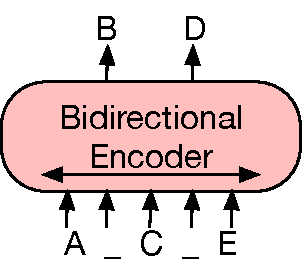
\includegraphics[width=0.7\linewidth]{obrazky-figures/lm_archs/bert.pdf}
        \vspace{0.5em} % Space between image and text
        \parbox{\linewidth}{\small % Use parbox for text wrapping within minipage
        (a) BERT: Random tokens are replaced with masks, and the document is encoded bidirectionally. Missing tokens are predicted independently, so BERT cannot easily be used for generation.
        }
    \end{minipage}
    \hfill % Space between BERT and GPT
    % --- GPT Subfigure (b) ---
    \begin{minipage}[t]{0.48\textwidth}
        \centering
        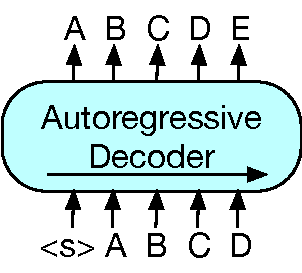
\includegraphics[width=0.7\linewidth]{obrazky-figures/lm_archs/gpt.pdf}
        \vspace{0.5em} % Space between image and text
        \parbox{\linewidth}{\small % Use parbox for text wrapping within minipage
        (b) GPT: Tokens are predicted auto-regressively, meaning GPT can be used for generation. However words can only condition on leftward context, so it cannot learn bidirectional interactions.
        }
    \end{minipage}

    \vspace{1em} % Vertical space before BART

    % --- BART Subfigure (c) ---
    \begin{minipage}[t]{\textwidth} % Use full width for BART for better centering/text flow
        \centering
        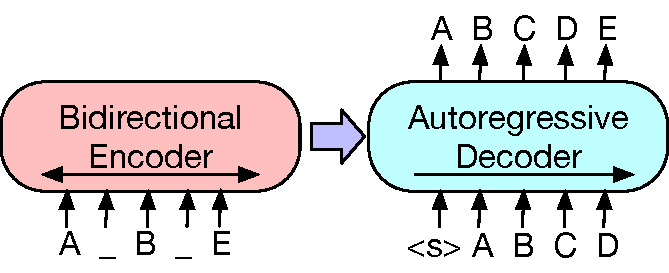
\includegraphics[width=0.7\linewidth]{obrazky-figures/lm_archs/bart.pdf} % Adjusted width as per original fbox
        \vspace{0.5em} % Space between image and text
        \parbox{0.9\linewidth}{\small % Use parbox for text wrapping, slightly narrower than full width
        (c) BART: Inputs to the encoder need not be aligned with decoder outputs, allowing arbitrary noise transformations. Here, a document has been corrupted by replacing spans of text with mask symbols. The corrupted document (left) is encoded with a bidirectional model, and then the likelihood of the original document (right) is calculated with an autoregressive decoder. For fine-tuning, an uncorrupted document is input to both the encoder and decoder, and we use representations from the final hidden state of the decoder.
        }
    \end{minipage}

    \caption{A schematic comparison of BART \cite{lewis2019bartdenoisingsequencetosequencepretraining} with BERT (\cite{devlin2018bert}) and GPT (\cite{radford2018improving}). Cited from \cite{lewis2019bartdenoisingsequencetosequencepretraining}.}
    \label{fig:model_comparison_schematics} % Label for the overall figure
\end{figure}


\subsection{Bidirectional and Auto-Regressive Transformer (BART)}
\label{subsec:bart}

BART (Bidirectional and Auto-Regressive Transformers) \cite{lewis2019bartdenoisingsequencetosequencepretraining} is an encoder-decoder language model designed for sequence-to-sequence tasks. It conceptualizes pre-training as a denoising autoencoder task. BART is trained using text corruption and reconstruction, as detailed above in \ref{corupt_enum}.

Architecturally, BART utilizes a standard transformer encoder-decoder setup \cite{vaswani2017attention}. It employs a bidirectional encoder to process the potentially corrupted input sequence. This is coupled with an autoregressive decoder (similar to GPT) which generates the output sequence.

An innovation in BART's pre-training is the flexibility of the noising schemes applied to the input text. The authors experimented with several corruption strategies, finding the best performance often came from combining multiple approaches. 
By learning to reverse these diverse corruptions, BART develops robust representations suitable for a wide range of tasks. While particularly effective for generative tasks like abstractive summarization, dialogue, and machine translation due to its autoregressive decoder, BART also demonstrates strong performance on comprehension tasks like SQuAD and GLUE \cite{lewis2019bartdenoisingsequencetosequencepretraining}. In the context of ASR, the decoder component of BART can be leveraged for its strong language modeling capabilities but also because its architecture inherently includes the cross-attention mechanism necessary for conditioning on acoustic encoder representations.

\subsection{Generative Pre-trained Transformer (GPT)}
\label{subsec:gpt}

The Generative Pre-trained Transformer (GPT) series of models represents a family of decoder-only language models. These models are built upon the decoder part of the standard transformer architecture \cite{vaswani2017attention}.

The fundamental pre-training objective for GPT models is Causal Language Modeling (CLM), or next-token prediction. Given a sequence of tokens \(s_1, \dots, s_{n-1}\), the model is trained to maximize the likelihood of the next token \(s_n\):
\begin{equation}
    L_{\text{CLM}} = \sum_i \log P(s_i | s_1, \dots, s_{i-1}; \Theta)
\end{equation}
where \(\Theta\) denotes the trainable parameters of the language model.

The GPT series has demonstrated a clear trend: increasing model size, dataset size, and training compute leads to improved performance. The original GPT \cite{radford2018improving} introduced the effectiveness of the generative pre-training approach followed by task-specific fine-tuning for various NLP benchmarks. Subsequently, GPT-2 \cite{radford2019language} scaled the model size significantly (up to 1.5 billion parameters) and was trained on a large, curated web text dataset (WebText); it demonstrated remarkable zero-shot learning capabilities, performing various tasks without any explicit fine-tuning, simply by conditioning the model with appropriate prompts. Further scaling occurred with GPT-3 \cite{brown2020languagemodelsfewshotlearners}, which reached up to 175 billion parameters and was trained on even more extensive data. Its key contribution was demonstrating powerful few-shot (or "in-context") learning; by providing just a few examples of a task within the prompt at inference time, GPT-3 could often match or exceed the performance of state-of-the-art fine-tuned models on various benchmarks without requiring any gradient updates or parameter changes. Subsequent models, such as GPT-4 \cite{openai2023gpt4} and GPT-4o \cite{openai2024gpt4o}, have continued this scaling trend, incorporating multimodal capabilities and enhanced reasoning abilities; however, these models remain closed-source.


\section{Pre-trained Acoustic Models}
Similar to the advances seen in natural language processing, pre-trained acoustic models have become essential to speech processing. Leveraging the idea of self-supervised learning, these models are initially trained to extract meaningful, high-level representations from large quantities of unlabeled audio data. Subsequently, the pre-trained model is fine-tuned on a smaller, labeled dataset for a specific downstream task, such as automatic speech recognition (ASR), speaker identification, emotion recognition, or language identification. This two-stage approach is advantageous when labeled data is scarce, which is common for many of the world's languages and specialized domains. This section will focus on the influential Wav2Vec 2.0 architecture and more recent models.


\subsection{Wav2Vec 2.0}\label{theory_wav2vec2}
Wav2Vec 2.0 represents a milestone in self-supervised learning for speech representations. It demonstrated that learning powerful representations directly from raw audio, followed by fine-tuning, outperforms previous state-of-the-art methods. The idea is to learn speech representations by solving a contrastive task in the latent space, analogous to masked language modeling in NLP.

\subsubsection{Architecture}

The Wav2Vec 2.0 model architecture as illustrated in Figure \ref{fig:wav2vec2_arch}, consists of three main components:

\begin{figure}[h!]
    \centering
    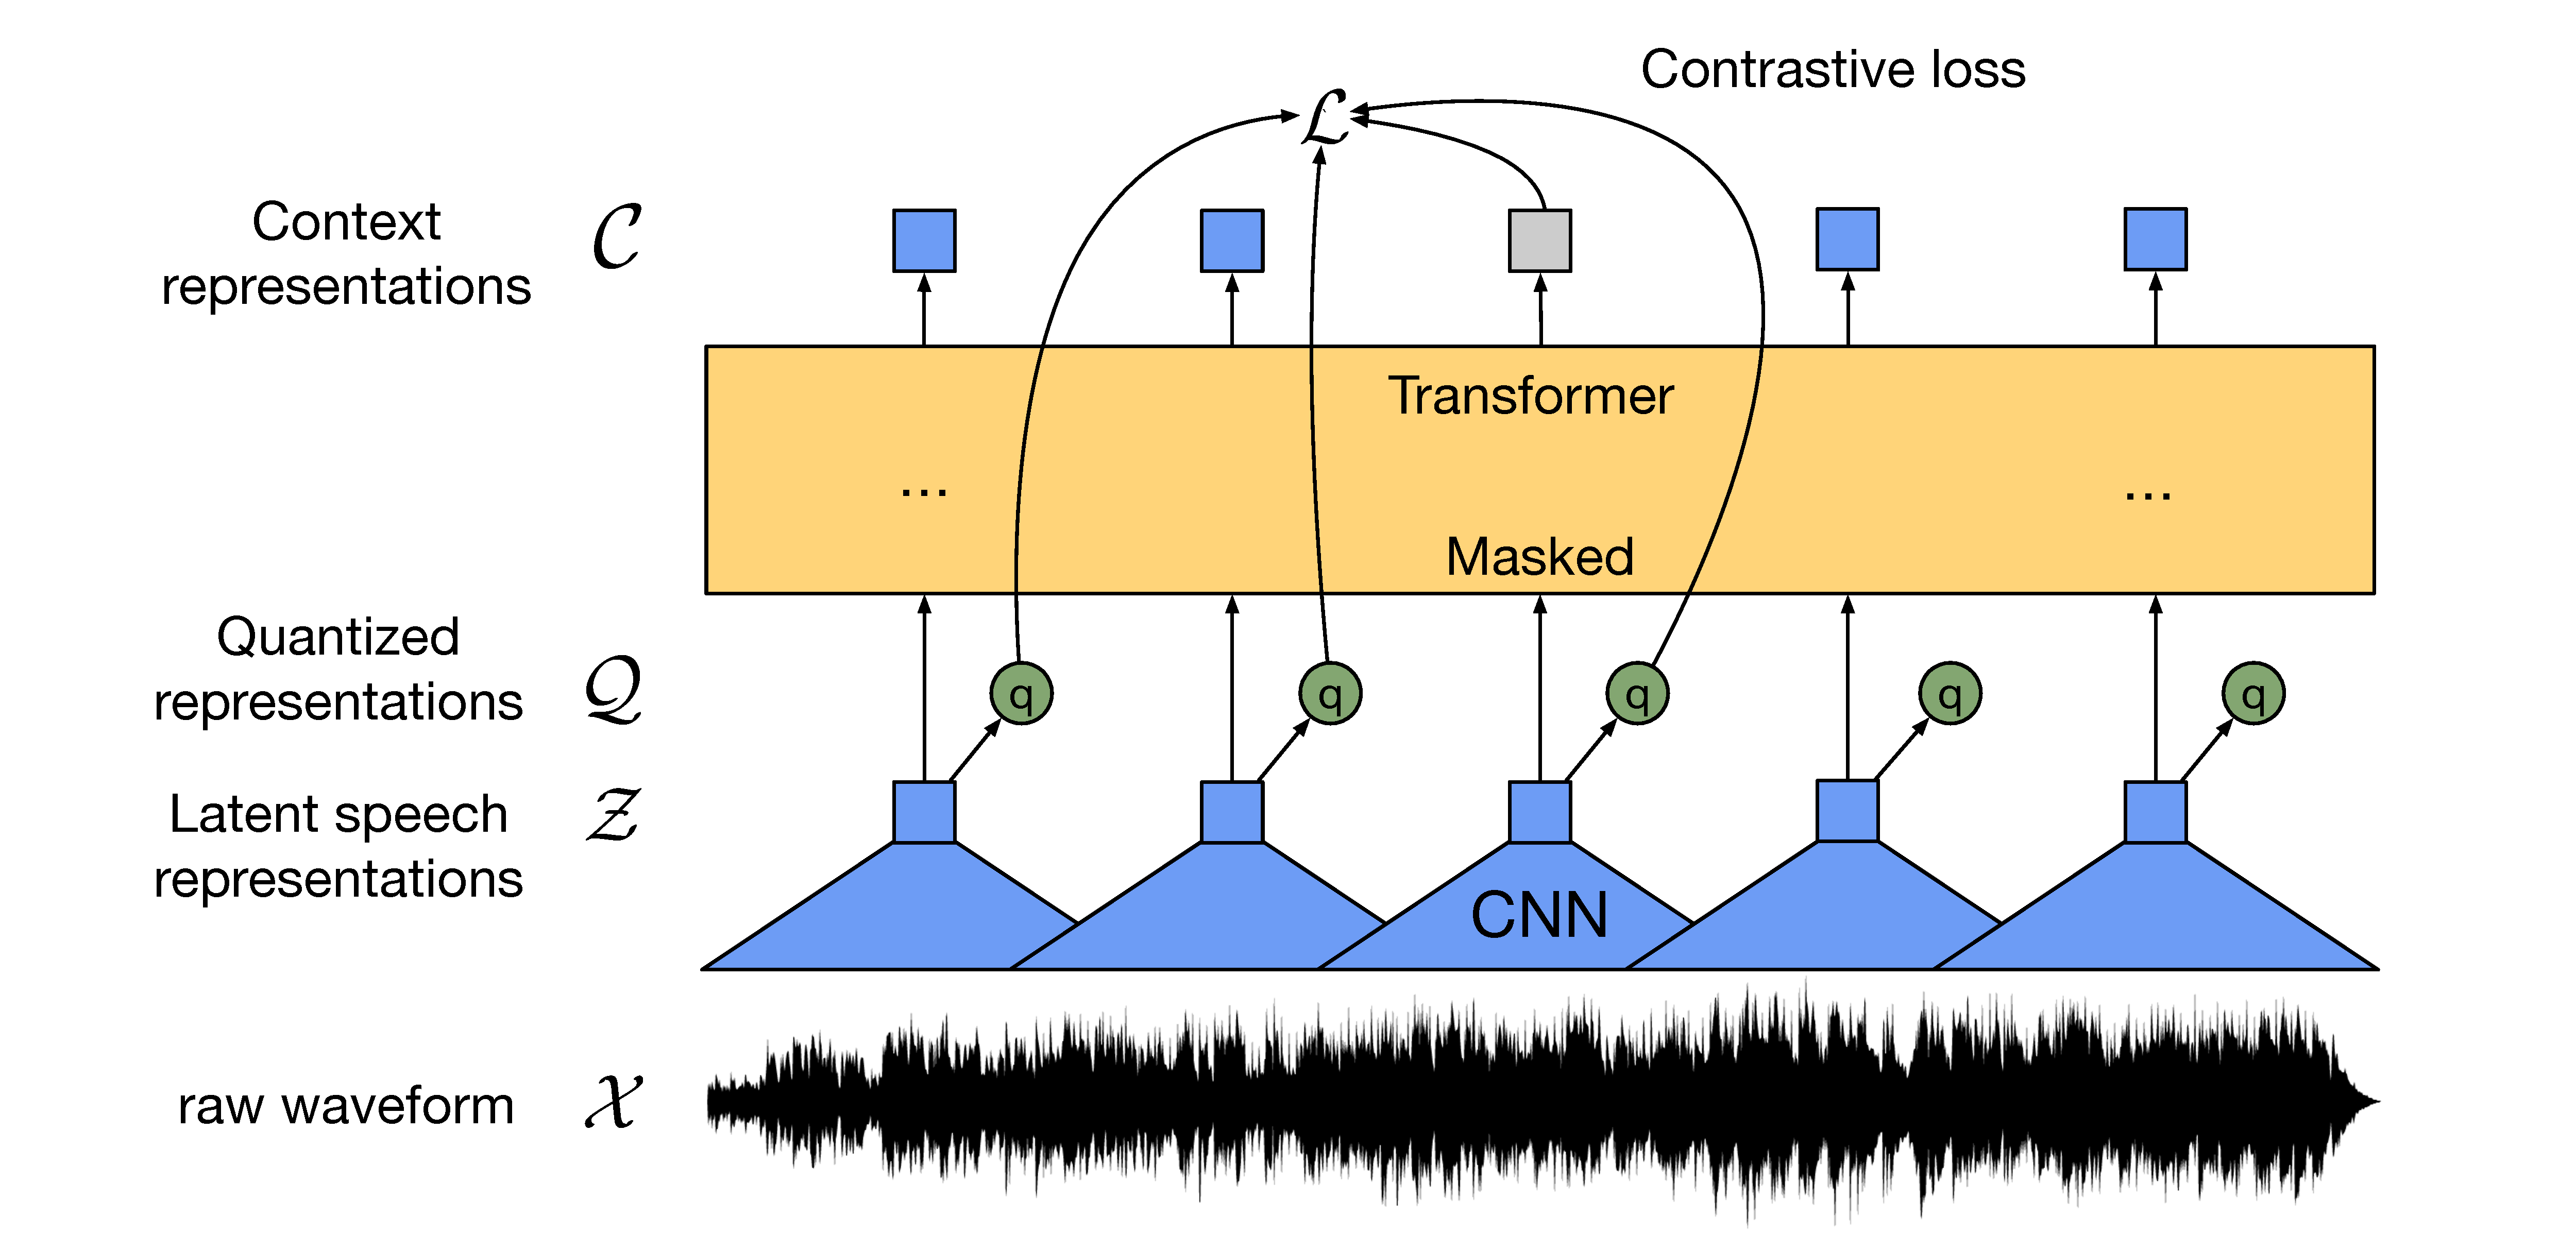
\includegraphics[width=1\textwidth]{obrazky-figures/wav2vec2/wav2vec2.pdf}
    \caption{The Wav2Vec 2.0 framework architecture, showing the feature encoder (CNN), transformer network, and quantization module used during pre-training. Adapted from \cite{baevski2020wav2vec20frameworkselfsupervised}.}
    \label{fig:wav2vec2_arch}
\end{figure}

\begin{enumerate}
    \item \textbf{Feature Encoder}: This module consists of a multi-layer 1D convolutional neural network (CNN) \( f: \mathcal{X} \mapsto \mathcal{Z} \). It takes the raw audio waveform \( \mathcal{X} \) as input and produces a sequence of latent speech representations \( \mathbf{Z} = (z_1, \dots, z_T) \) at a lower temporal frequency (every 20ms). The encoder captures local acoustic features. In the BASE (smaller) configuration, this part has seven blocks with temporal convolutions, resulting in a receptive field of 25 ms.

    \item \textbf{Context Network (Transformer)}: The sequence of latent representations \( \mathbf{Z} \) is then fed into a standard transformer network \( g: \mathcal{Z} \mapsto \mathcal{C} \). This network applies multi-head self-attention to capture contextual dependencies over the entire sequence, which then produces context-aware representations \( \mathbf{C} = (c_1, \dots, c_T) \). Unlike standard transformers, Wav2Vec 2.0 replaces fixed positional embeddings with a convolutional layer to learn relative positional information. The BASE model uses 12 transformer blocks, while the larger variant (LARGE) uses 24 blocks.

    \item \textbf{Quantization Module}: This module discretizes the output of the feature encoder \( \mathbf{Z} \) into a finite set of codebook entries \( \mathbf{Q} = (q_1, \dots, q_T) \). This is achieved using product quantization, where each latent vector \( z_t \) is mapped to \( G \) codebooks, each containing \( V \) entries. The selected entries are concatenated and linearly transformed to form \( q_t \). Crucially, this module is only used during the self-supervised pre-training phase to generate targets for the contrastive task. Wav2Vec 2.0 employs Gumbel-Softmax \cite{jang2016categorical} to allow differentiable selection of codebook entries during training. The probability of choosing the \( v \)-th codebook entry for group \( g \) is given by:
    \begin{equation} \label{eq:gumbel_softmax}
        p_{g,v} = \frac{\exp(l_{g,v} + n_v)/\tau}{\sum_{k=1}^{V} \exp(l_{g,k} + n_k)/\tau}
    \end{equation}
    where \( l \) are the logits computed from \( z_t \), \( n = -\log(-\log(u)) \) with \( u \sim U(0, 1) \) are Gumbel noise samples, and \( \tau \) is a non-negative temperature parameter that is annealed during training.
\end{enumerate}

\subsubsection{Self-Supervised Pre-training}

Wav2Vec 2.0 is pre-trained on large amounts of unlabeled speech audio using a contrastive task combined with a diversity loss.

\begin{enumerate}
    \item \textbf{Masking}: Similarly to BERT, a portion of the latent feature encoder outputs \( \mathbf{Z} \) is masked before being fed into the transformer context network. Specifically, a proportion \( p \) (\( p=0.065 \)) of time steps is randomly selected as starting indices. Each selected index initiates a mask over the subsequent \( M \) time steps (\( M=10 \)). These masked latent vectors \( z_t \) are replaced with a single learned feature vector representation before entering the transformer. This masking strategy results in approximately 49\% of the total time steps being masked \cite{baevski2020wav2vec20frameworkselfsupervised}.

    \item \textbf{Contrastive Loss}: For each masked time step \( t \), the model uses the corresponding contextualized representation \( c_t \) from the transformer output to predict the correct quantized representation \( q_t \) (derived from the unmasked \( z_t \) via the quantization module). The prediction is framed as a contrastive task: identifying the true target \( q_t \) from a set of \( K \) distractor quantized representations \( \tilde{q} \). These distractors are uniformly sampled from other masked time steps within the same audio utterance. The contrastive loss \( \mathcal{L}_m \) is defined as:
    \begin{equation} \label{eq:contrastive_loss}
        \mathcal{L}_m = -\log \frac{\exp(\text{sim}(c_t, q_t)/\kappa)}{\sum_{\tilde{q} \sim Q_t} \exp(\text{sim}(c_t, \tilde{q})/\kappa)}
    \end{equation}
    where \( \text{sim}(a, b) = \mathbf{a}^\top \mathbf{b} / (\|\mathbf{a}\| \|\mathbf{b}\|) \) is the cosine similarity, \( Q_t \) is the set containing \( q_t \) and the \( K \) distractors (\(K=100\)), and \( \kappa \) is a temperature parameter \cite{baevski2020wav2vec20frameworkselfsupervised}.

    \item \textbf{Diversity Loss}: To encourage the model to utilize the codebook entries effectively, a diversity loss \( \mathcal{L}_d \) is added. This loss maximizes the entropy of the averaged softmax distribution of codebook usage across batches for each codebook group \( G \). Let \( \bar{p}_{g,v} \) be the average probability of using the \( v \)-th entry in the \( g \)-th codebook. The diversity loss is:
    \begin{equation} \label{eq:diversity_loss}
        \mathcal{L}_d = \frac{1}{GV} \sum_{g=1}^{G} -H(\bar{p}_g) = \frac{1}{GV} \sum_{g=1}^{G} \sum_{v=1}^{V} \bar{p}_{g,v} \log \bar{p}_{g,v}
    \end{equation}
    This loss term encourages the model to explore and utilize the full capacity of the quantization codebooks.
\end{enumerate}

The overall pre-training objective is a weighted sum of the contrastive loss and the diversity loss:
\begin{equation} \label{eq:total_pretrain_loss}
    \mathcal{L} = \mathcal{L}_m + \alpha \mathcal{L}_d
\end{equation}
where \( \alpha \) is a hyperparameter controlling the weight of the diversity loss (\( \alpha=0.1 \)) \cite{baevski2020wav2vec20frameworkselfsupervised}.

\subsubsection{Fine-tuning for ASR}

After pre-training on unlabeled data, the Wav2Vec 2.0 model is fine-tuned for ASR using labeled data. A randomly initialized linear layer is added on top of the transformer output \( \mathbf{C} \) to predict the vocabulary tokens (characters or sub-words). The model is then trained using the CTC~\ref{ctc_theory} loss. During fine-tuning, the parameters of the transformer and the new linear layer are updated. The quantization module is not used during fine-tuning.

The success of Wav2Vec 2.0 comes from its ability to learn representations directly from raw audio waveforms in a self-supervised manner, which reduces the need for large amounts of transcribed data.


\subsection{Whisper}
Representing a different paradigm and architecture compared to self-supervised models such as Wav2Vec2, Whisper \cite{radford2022robust}, developed by OpenAI, leverages large-scale weakly supervised pretraining for multilingual and multitask speech recognition. Instead of learning from unlabeled audio, Whisper v1 is trained on a dataset of 680,000 hours of audio paired with noisy transcripts collected from the internet. The core goal of Whisper was to build a robust model capable of strong zero-shot generalization across different datasets, tasks, and languages without the need for task-specific fine-tuning.

\subsubsection{Architecture}
Whisper uses a transformer encoder-decoder architecture. Input is a raw audio waveform, which is resampled to 16 kHz. An 80-channel log-magnitude Mel spectrogram is computed using 25-millisecond windows with a 10-millisecond stride, serves as the input to the encoder. The encoder architecture features a small convolutional \textit{stem} that consists of two 1D convolutional layers with GELU activation \cite{hendrycks2016gaussian} where the second layer has a stride of two, to initially process the spectrogram. Sinusoidal positional embeddings are added to the output of this \textit{stem} before the features are passed into the main transformer blocks, which utilize pre-activation residual connections. The decoder uses learned positional embeddings and employs tied input-output token representations \cite{Press_2017}. For tokenization, they utilize a byte-level Byte-Pair Encoding tokenizer, identical in principle to the one used for GPT-2 but specifically refitted for multilingual data. OpenAI has released this architecture in several sizes, ranging from a \texttt{tiny} model with 39 million parameters up to a \texttt{large} version containing 1.55 billion parameters. The architecture is illustrated in Figure \ref{fig:whisper_format}.


\begin{figure}[h!]
    \centering
    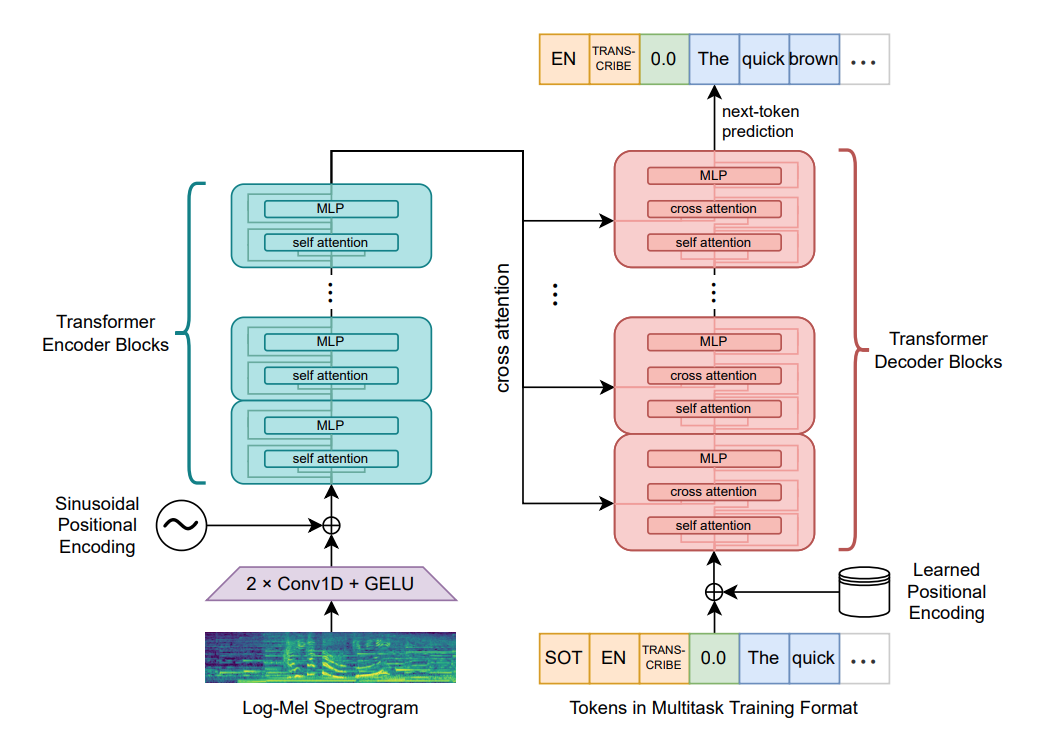
\includegraphics[width=1\textwidth]{obrazky-figures/whisper_arch.png} 
    \caption{Overview of the Whisper architecture. Figure adapted from \cite{radford2022robust}.}
    \label{fig:whisper_format}
\end{figure}

\subsubsection{Recent Developments and Relevance to Encoder-Decoder ASR}
Since its initial release, Whisper has seen several iterations and inspired community-driven improvements. Whisper v2 incorporated longer training with regularization techniques (SpecAugment~\cite{Park2019SpecAugment}, Stochastic Depth~\cite{Stochastic_depth} and BPE Dropout~\cite{Provilkov_2020}. Subsequently, Whisper v3 was trained on a substantially larger and more diverse dataset, leveraging 1 million hours of weakly labeled audio and 4 million hours of pseudo-labeled audio. Along with minor architectural refinements (128 Mel frequency bins), this extensive data foundation contributed to further WER reductions of 10-20\% over v2, particularly by improving its multilingual capabilities~\cite{huggingface_whisper_large_v3_card}.

Fine-tuned variants have also emerged. CrisperWhisper \cite{zusag2024crisperwhisper} focuses on verbatim transcription by employing an adjusted tokenizer and a custom attention loss during fine-tuning to achieve accurate word-level timestamps, differentiate spoken fillers ("um," "uh"), and transcribe speech exactly as uttered. CrisperWhisper shows stronger performance on the ASR leaderboard \cite{open-asr-leaderboard} than Whisper v3.

Whisper serves as a prominent example of an encoder-decoder architecture for ASR that integrates acoustic encoding with autoregressive textual generation. This architectural choice differs from encoder-only approaches. An understanding of the capabilities and structure of models like Whisper is relevant, as this thesis investigates techniques relevant to the effective training and adaptation of encoder-decoder models for speech recognition tasks.


\subsection{Canary}\label{subsec:canary}

The model that achieves the highest scores across many datasets is called Canary \cite{puvvada2024accurate} and was released by NVIDIA. They challenge the reliance on web-scale datasets for training high-performance ASR models. This encoder-decoder model exceeds Whisper-large-v3 on benchmarks for English, French, Spanish, and German, while using considerably less training data (around 86,000 hours versus Whisper's initial 680,000+ hours). Architecturally, Canary utilizes a FastConformer encoder paired with a standard transformer decoder. Key training differences contributing to its performance with less data include the use of pseudo-labeled translation data for AST, data balancing and dynamic bucketing techniques (reducing computational overhead and speeding up training compared to fixed-length padding used in Whisper training), initializing the encoder from a pre-trained ASR checkpoint, and incorporating noise-robust fine-tuning which reduces model hallucinations. Canary achieves strong accuracy with less data and faster training, completing in under 48 hours on 128 A100 GPUs.


\section{Parameter-Efficient Fine-tuning}\label{sec:peft}

Training large-scale models, such as the transformer-based architectures prevalent in both acoustic and language modeling for ASR, demands substantial computational resources and memory. Full fine-tuning, where all model parameters are updated on a downstream task, becomes increasingly impractical as model sizes grow into billions of parameters. Parameter-Efficient Fine-tuning (PEFT) techniques have emerged as a crucial solution to this challenge \cite{ding2023parameter}. PEFT methods aim to adapt large pre-trained models to specific tasks or domains by training only a small fraction of the total parameters or only a small number of additional parameters. This significantly reduces the computational cost, memory requirements, and storage overhead associated with fine-tuning, while often achieving performance comparable to full fine-tuning \cite{lialin2023scaling}. They preserve the knowledge captured during pre-training and reduce the risk of catastrophic forgetting and overfitting, especially when the fine-tuning dataset is small \cite{xu2023parameterefficient}.

In the context of ASR, state-of-the-art ASR relies on massive pre-trained acoustic models and potentially large language models. Adapting these models to specific languages, accents, domains (medical dictation, call center conversations), or even individual speakers using full fine-tuning is, in many cases, impractical. PEFT allows for efficient specialization of these powerful pre-trained models.


The landscape of PEFT methods is diverse and rapidly evolving. These techniques can be broadly categorized based on how they modify the model during fine-tuning. PEFT methods can be classified into several major groups: additive, partial, reparameterized, hybrid, and unified fine-tuning \cite{xu2023parameterefficient}.


\subsection{Additive Fine-tuning}
These methods introduce new, trainable parameters or modules into the architecture while keeping the original parameters frozen.

\begin{itemize}
    \item \textbf{Adapter-based Fine-tuning}: This approach involves inserting small, task-specific neural network modules, known as adapters, into the layers of the pre-trained model. Typically, these are small feed-forward networks (often with a bottleneck structure: down-projection -> non-linearity -> up-projection) placed after the attention and feed-forward layers in each transformer block \cite{houlsby2019parameterefficient}. Variations include placing adapters in parallel \cite{he2021unified}, using residual connections \cite{Lin_2020}, dynamically dropping adapters during inference \cite{ruckle-etal-2021-adapterdrop}, fusing knowledge from multiple adapters \cite{pfeiffer-etal-2021-adapterfusion}, or using hypernetworks to generate adapter parameters \cite{he2022hyperprompt}.

    \item \textbf{Soft Prompt-based Fine-tuning}: Instead of modifying internal model weights, these methods prepend trainable continuous vectors (soft prompts or prefixes) to the input embedding sequence or intermediate hidden states. Prompt Tuning \cite{lester-etal-2021-power} adds learnable prompt tokens directly to the input embeddings. Prefix Tuning \cite{li-liang-2021-prefix} adds trainable prefix vectors to the hidden states within each layer's attention mechanism (affecting keys and values). Other methods explore variations like adversarial prompts or multi-task prompt transfer. In this variant, only the prompt/prefix vectors are trained.

    \item \textbf{Other Additive Methods}: This category includes techniques like Ladder Side-Tuning \cite{sung2022lst}, which adds a separate side network or (IA)\(^3\), that learns scaling vectors for activations \cite{liu2022fewshot}.
\end{itemize}

\subsection{Partial Fine-tuning}
These methods fine-tune only a selected subset of the original pre-trained parameters, keeping the rest frozen.

\begin{itemize}
    \item \textbf{Bias Update}: Techniques like BitFit \cite{zaken2021bitfit} propose fine-tuning only the bias terms within the transformer layers and the classification head. This is extremely parameter-efficient but it has limited expressivity. 
    \item \textbf{Pretrained Weight Masking}: Methods like Threshold-Mask \cite{Zhao_2020} or FISH Mask \cite{sung2021training} identify important pre-trained weights based on criteria like magnitude or Fisher information and create a binary mask. Only unmasked weights are active or used. Typically, the weights remain frozen, and the mask selects them.
    \item \textbf{Delta Weight Masking}: These methods focus on masking the updates (delta weights) applied to the pre-trained weights. LT-SFT \cite{Ansell_2022} identifies parameters with large changes after initial full fine-tuning and only tunes those in subsequent steps. Diff Pruning \cite{guo-etal-2021-parameter} learns a sparse mask for the delta weights directly. SAM \cite{fu2022effectiveness} uses a second-order approximation to select delta weights.
\end{itemize}

\subsection{Reparameterized Fine-tuning}
This category, which includes LoRA and its derivatives, modifies the model by reparameterizing the weight update matrices, often using low-rank matrices.

\begin{itemize}
    \item \textbf{Low-rank Decomposition}: This involves approximating the weight update matrix \( \Delta W \) as a product of smaller matrices.
        \begin{itemize}
            \item \textbf{LoRA (Low-Rank Adaptation)}\label{lora_theory} \cite{hu2021lora}: This has become a very popular and effective technique. It hypothesizes that the change \( \Delta W \) needed to adapt a pre-trained weight matrix \( W \in \mathbb{R}^{d \times k} \) is low-rank. LoRA introduces two small, trainable matrices \( B \in \mathbb{R}^{d \times r} \) and \( A \in \mathbb{R}^{r \times k} \), where the rank \( r \ll \min(d, k) \), such that the update is \( \Delta W = BA \). The effective weight matrix used during fine-tuning is \( W' = W + \Delta W \), often with a scaling factor:
                  \begin{equation}
                      W' = W + \frac{\alpha}{r} BA
                      \label{eq:lora_update_peft}
                  \end{equation}
                  Only \( A \) and \( B \) are trained, while the original \( W \) is frozen. This drastically reduces the number of trainable parameters to \( r(d+k) \). A significant advantage is that after training, \( \Delta W \) can be merged with \( W \) (\( W_{\text{merged}} = W + \frac{\alpha}{r} BA \)), resulting in zero additional inference latency compared to the original model. LoRA is commonly applied to attention weight matrices (Query, Key, Value, Output) and sometimes Feed-Forward Network layers.

                  However, LoRA introduces potential limitations. The low-rank constraint may restrict the expressiveness of the weight updates, potentially limiting adaptation to tasks requiring significant deviations from the pre-trained model. Additionally, the choice of hyperparameters $r$ and $\alpha$ can affect stability and performance, with excessively large updates risking training divergence \cite{hu2021lora}.
            \item \textbf{KronA (Kronecker Adapter)} \cite{edalati2022krona}: Uses Kronecker products instead of standard matrix multiplication for the decomposition \( \Delta W = B \otimes A \).
        \end{itemize}

    \item \textbf{LoRA Derivatives}: Building on the success and simplicity of LoRA, numerous derivative techniques have emerged to address its limitations or enhance its capabilities in specific scenarios. Key directions include improving efficiency through quantization and optimizing parameter allocation.
            \begin{itemize}
                \item \textit{Quantization-Aware Adaptation}: QLoRA \cite{dettmers2023qlora} reduces the memory footprint required for fine-tuning. QLoRA achieves this by quantizing the pre-trained model weights to very low precision, typically 4-bit. While the base model is quantized, the LoRA adapter weights are kept in a higher precision format. During the forward pass, the quantized base weights are de-quantized on-the-fly to the compute precision, the LoRA update is computed and added, and then the computation proceeds. To further save memory, QLoRA employs techniques like double quantization and paged optimizer (offloading optimizer states to CPU RAM). Other related work, like QA-LoRA \cite{xu2023qalora} and LOFTQ \cite{li2023loftq}, explores integrating quantization more deeply into the LoRA process for potentially faster inference or better initialization.
    
                \item \textit{Adaptive Rank Allocation (AdaLoRA)}: Standard LoRA uses a fixed rank \(r\) for all adapted matrices. However, different layers or matrices might benefit from different adaptation capacities. AdaLoRA \cite{zhang2023adalora} addresses this by dynamically allocating the parameter budget (the rank) during training based on the importance of weight matrices. It parameterizes the LoRA update using Singular Value Decomposition (SVD) and adaptively prunes less important singular values based on a sensitivity-based importance score. This allows the model to allocate more parameters (higher rank) to weight matrices that contribute more significantly to the task, while reducing the rank for less important ones.
    
                \item \textit{Other Variations}: Further research has explored aspects like pruning within LoRA (LoRAPrune \cite{Zhang_2024}), incorporating Bayesian principles (Laplace-LoRA \cite{yang2023bayesian}), or modifying the update mechanism itself, such as freezing one of the LoRA matrices to save activation memory (LoRA-FA \cite{zhang2023lorafa}) or decomposing the update differently (DoRA \cite{liu2024dora}).
            \end{itemize}
    \end{itemize}

\subsection{Weight-Decomposed Low-Rank Adaptation (DoRA)}\label{dora_theory}
DoRA \cite{liu2024dora} is a recent technique that refines LoRA by explicitly decomposing the pre-trained weight matrix \( W_0 \) into magnitude and direction components before applying the low-rank update. The idea is to separate the adaptation of how much a neuron fires (magnitude) from what pattern it responds to (direction).
First, \( W_0 \) is decomposed:
\begin{equation}
    W_0 = m \odot \frac{V}{||V||_c} \approx m \odot \frac{W_0}{||W_0||_c}
    \label{eq:dora_decomposition_peft_2}
\end{equation}
where \( m \) is a learnable vector representing the column-wise magnitude, \( V \) is the directional component (initialized as \( W_0 \)), \( ||\cdot||_c \) is the column-wise norm, and \(\odot\) denotes element-wise multiplication.
Fine-tuning involves updating both \( m \) and \( V \). Importantly, the low-rank update \( \Delta V = BA \) (using LoRA matrices A and B with rank \( r \)) is applied only to the directional component \( V \):
\begin{equation}
    W' = m \odot \frac{V + \Delta V}{||V + \Delta V||_c} = m \odot \frac{W_0 + BA}{||W_0 + BA||_c}
    \label{eq:dora_finetune_peft_2}
\end{equation}
Here, the trainable parameters are the magnitude vector \( m \) and the LoRA matrices \( B \) and \( A \). By explicitly learning the magnitude and applying LoRA to the normalized direction, DoRA aims for more stable and effective adaptation compared to standard LoRA, potentially capturing changes that LoRA might struggle with. However, unlike LoRA, the DoRA update cannot be easily merged back into \( W_0 \) for inference due to the dependence on the learned magnitude \( m \) and the normalization, which may introduce slight inference overhead.

\subsection{Hybrid Fine-tuning}
These methods manually combine different PEFT techniques to leverage their complementary strengths. Examples include MAM Adapter \cite{he2021unified} that combines parallel adapters and prefix-tuning) or UniPELT \cite{mao2021unipelt} that integrates sequential adapters, prefix-tuning, and LoRA with a gating mechanism.

\subsection{Unified Fine-tuning}
These approaches aim to create frameworks that can encompass or automatically select/configure different PEFT strategies. AutoPEFT \cite{Zhou_2024} uses Bayesian optimization to search for optimal configurations of adapters and prefix-tuning across layers. S\(^3\)Delta-M \cite{NEURIPS2022_4027fc45} performs differentiable structure search over combinations of methods like LoRA, Compacter, BitFit, etc.


\subsection{Summary of PEFT Approaches}
The choice of PEFT technique involves trade-offs between parameter efficiency, downstream task performance, training stability and speed, memory usage, implementation complexity, and potential inference overhead. Additive methods like adapters and prompt/prefix tuning are conceptually simple but might add inference latency or have limited capacity. Partial methods like BitFit are extremely efficient but may underperform. Reparameterized methods, particularly LoRA and its advanced derivatives like QLoRA and DoRA, offer a strong balance by significantly reducing trainable parameters while often matching full fine-tuning performance and allowing zero-cost inference merging. Hybrid and unified methods attempt to get the best of multiple worlds but can increase complexity.




\chapter{Experimental Evaluations}\label{experimentos}

This chapter details all the experiments in chronological order.  

\section{Model Selection}
For the experiments, I take advantage of \textit{transformers} library from huggingface and their class (SpeechEncoderDecoder \cite{huggingface2025transformers}) to directly use any encoder and decoder part. I choose the following transformer architectures for each part:

\subsection{Encoder}
The encoder is based on the \textit{Wav2Vec2} architecture described in Section \ref{theory_wav2vec2}, which showed that it can derive robust audio features from raw waveforms through self-supervised learning. Pre-training leveraged tens of thousands of hours of unlabeled speech, primarily sourced from LibriVox~\cite{Kahn_2020} dataset (providing over 53,000 hours), which allowed the model to develop robust representations effective across diverse real-world audio environments. The specific version chosen is \textit{base}, which is the smallest version, containing 12 transformer blocks, 768 model dimensions, inner dimension of size 3072 and 8 attention heads. The total size of the encoder is 105M parameters. 

\subsection{Decoder}
The decoder is based on \textit{BART} architecture, as described in Section \ref{subsec:bart}, which is an encoder-decoder model created for sequence-to-sequence generation tasks. The total size of the decoder is 96M parameters. 

The selection of \textit{BART} as the decoder, paired with the \textit{Wav2Vec2} encoder, was made after considering alternative architectures, including decoder-only models (e.g., GPT-2 variants) and other encoder-decoder frameworks (e.g., T5). A primary constraint in this selection was the requirement for the decoder's parameter count to be comparable to that of the \textit{Wav2Vec2} encoder. The employed \textit{BART} model satisfies this constraint. Furthermore, this specific \textit{Wav2Vec2}-\textit{BART} integration directly aligns with the methodology used by von Platen et  al. \cite{vonPlaten2020warmstart}, which demonstrated the efficacy of leveraging these pre-trained components for ASR. This architectural choice capitalizes on the complementary strengths of \textit{Wav2Vec2} for robust acoustic feature extraction and \textit{BART}'s proficiency in generating coherent textual output.
From \textit{BART} architecture, only the decoder part is used. Convolutional adapter layers are added in the encoder to align the output with the decoder. 

\section{Dataset and Preprocessing}\label{sec:dataset_preprocessing_exp}

The performance, robustness, and generalization capabilities of the techniques explored in this thesis are reliant on the data used for training and evaluation. High-quality and sufficiently large datasets are key. Speech itself presents significant variability, influenced by factors that include language, regional accents, speaker demographics, speaking style, and recording conditions. This diversity demands various specialized datasets, each tailored to specific ASR tasks, languages, or acoustic environments.

The experiments in this thesis utilize two English language datasets: LibriSpeech and VoxPopuli. A summary of their key characteristics is presented in Table~\ref{tab:used_asr_datasets_exp}, followed by more detailed descriptions.

\begin{table}[h!]
    \centering
    \small
    \begin{tabular}{|l|l|l|}
        \hline
        \textbf{Dataset} & \textbf{Language (s)} & \textbf{Duration (hours)} \\
        \hline
        LibriSpeech & English & ~1,000 (Total Labeled) \\
        \hline
        VoxPopuli & English (Used Subset) & ~1,800 (Labeled EN) / ~400,000 (Total Unlabeled) \\
        \hline
    \end{tabular}
    \caption{Key characteristics of the primary ASR datasets utilized in this thesis.}
    \label{tab:used_asr_datasets_exp} % Changed label to avoid conflict if the old table still exists elsewhere
\end{table}

\subsection{Datasets Used in Experiments} % Or simply integrate into the main text of the section

\subsubsection{LibriSpeech}
LibriSpeech \cite{libri} is a widely adopted benchmark dataset for ASR research, particularly for evaluating models on clean, read English speech. It comprises recordings derived from audiobooks available through the LibriVox project. The audio is sampled at 16 kHz and is accompanied by high-quality transcriptions. Its large size and clean nature make it suitable for training and evaluating robust ASR models, although it primarily represents a single domain (audiobooks). For the experiments in this thesis, the `train-clean-100` subset (100 hours of the cleanest speech) is used for training, and the standard `dev-clean` and `test-clean` subsets are used for evaluation.

\subsubsection{VoxPopuli}
VoxPopuli \cite{wang2021voxpopulilargescalemultilingualspeech} offers a large-scale multilingual speech corpus sourced from European Parliament proceedings recorded between 2009 and 2020. It is significantly larger and more diverse than LibriSpeech in terms of languages and potentially speaking styles. The full dataset contains approximately 400,000 hours of unlabeled audio across 23 European languages. For supervised tasks, it includes 1,800 hours of transcribed speech data along with aligned text translations in up to 15 languages. This makes VoxPopuli valuable for multilingual ASR and tasks like speech translation and cross-lingual transfer learning. The experiments in this thesis focus on the labeled English portion of the dataset for training and evaluation.

\subsection{Data Preprocessing}

The audio data from both LibriSpeech and VoxPopuli is resampled to $16\,kHz$ to meet the input requirements of the \textit{Wav2Vec2} model. Text transcriptions are tokenized using the \textit{BART} tokenizer. This tokenizer employs a vocabulary of 50,265 tokens, which includes special tokens for start-of-sequence (\texttt{<s>}, ID: 0), end-of-sequence (\texttt{</s>}, ID: 2), and padding (\texttt{<pad>}, ID: 1).

\section{Evaluation Metric: Word Error Rate (WER)}
The Word Error Rate (WER) is a widely used metric to evaluate the performance of automatic speech recognition systems by measuring the discrepancy between the predicted transcription and the reference text. It accounts for three types of errors: substitutions, where an incorrect word is predicted in place of the correct one; deletions, where a word present in the reference is omitted in the prediction; and insertions, where an extra word is added to the prediction that does not appear in the reference. The WER is calculated using the following formula:

\[
\text{WER} = \frac{S + D + I}{N}
\]

Where, \(S\) represents the number of substitutions, \(D\) the number of deletions, \(I\) the number of insertions, and \(N\) the total number of words in the reference text. A lower WER indicates better performance, as it reflects fewer errors relative to the reference transcription.

The image below illustrates the components used to calculate the Word Error Rate by comparing Ground Truth text with Model output.

\begin{figure}[!h]
    \centering
    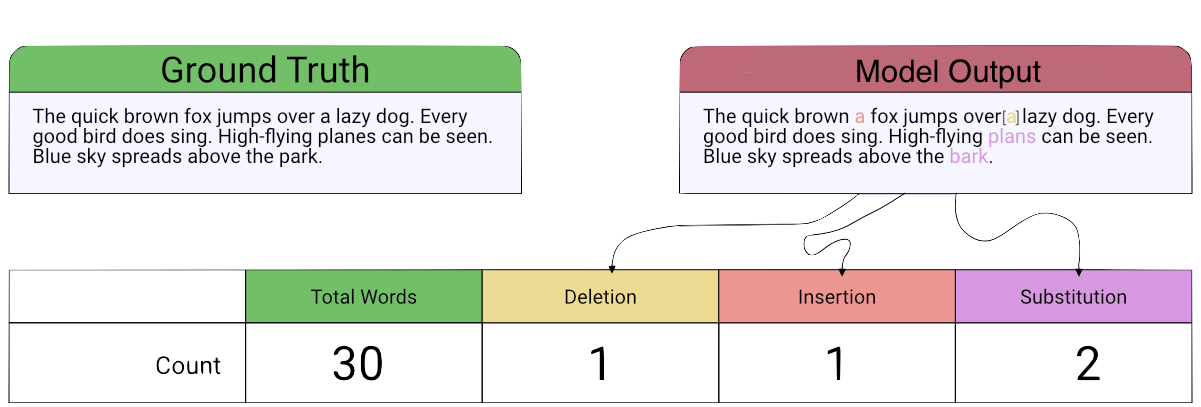
\includegraphics[width=0.9\textwidth]{obrazky-figures/werpls2.png}
    \caption{Comparison of Ground Truth and Model Output showing counts for Deletions (D), Insertions (I), and Substitutions (S). Image adapted from Martinez \cite{Martinez2025_OCRAccuracy}.}
    \label{fig:wer_calculation}
\end{figure}

Based on the counts shown in Figure \ref{fig:wer_calculation}: there were two substitutions, with 'planes' recognized as 'plans' and 'park' as 'bark'. There was one deletion, where the word 'a' before 'lazy' in the Ground Truth was missing in the Model output. Additionally, there was one insertion, as the word 'a' after 'brown' appeared in the Model output but not in the Ground Truth.


\section{Experimental Setup 1}
For the first experiment, I evaluate different initialization strategies for training a SpeechEncoderDecoder model for automatic speech recognition (ASR). The primary objective is to determine the impact of using pre-trained encoder and decoder components on model performance and training efficiency. Four different initialization strategies are evaluated:


\begin{enumerate}
    \item \textbf{Both Pretrained}: Both the encoder and decoder are initialized with pre-trained weights (\textit{Wav2Vec2-base} and \textit{BART-base}, respectively). Adapter layers in the encoder and Final linear layer (\texttt{lm\_head}) in the decoder are randomly initialized.
    \item \textbf{Pretrained Encoder}: The encoder is initialized with pre-trained \textit{Wav2Vec2-base} weights, while the decoder is randomly initialized.
    \item \textbf{Pretrained Decoder}: The decoder is initialized with pre-trained \textit{BART-base} weights, while the encoder is randomly initialized.
    \item \textbf{From Scratch}: Both the encoder and decoder are initialized at random.
\end{enumerate}

\subsection{Training Details}
\label{sec:experimental-setup-1}
The models are trained using the \textit{Seq2SeqTrainer} from the Hugging Face \textit{transformers} library. Training involves the use of the AdamW \cite{loshchilov2019decoupledweightdecayregularization} optimizer, paired with a cosine annealing scheduler that includes a linear warmup phase. Different learning rates are applied depending on the dataset and model configuration. For the LibriSpeech dataset, higher learning rates are used when both the encoder and decoder are pretrained; this reflects a fine-tuning scenario where the goal is primarily to adapt the robust pretrained representations and train the smaller, randomly initialized layers. However, lower learning rates are applied for cases with a pre-trained encoder, pre-trained decoder, or training from scratch. This provides the stability required to learn meaningful representations from scratch or to integrate a randomly initialized component with a pre-trained one without disrupting the latter's learned knowledge. Similarly, for the VoxPopuli dataset, learning rates vary across configurations with pretrained components or training from scratch. Batch sizes were set specifically for each dataset: 64 for LibriSpeech and 96 for the more extensive VoxPopuli dataset. Gradient accumulation is performed with a single step. The primary evaluation metric for assessing model performance was the WER.


\subsection{Results}
The performance of each initialization strategy on both datasets is summarized in the following tables:

\subsection*{LibriSpeech (clean.100)}
\begin{table}[h]
    \centering
    \begin{tabular}{@{} lccccccc @ {}}
    \toprule
    Initialization & WER [\%] ↓ & S & D & I & Eval Loss & Total Steps & Epochs \\
    \midrule
    \textbf{Both Pret.} & \textbf{8.9} & 7.2 & 0.9 & 0.8 & 0.57 & \textbf{2230} & 5 \\
    Pret. Encoder & 10.2 & 7.7 & 1.7 & 0.8 & 0.81 & 66900 & 150 \\
    Pret. Decoder & 106 & 81.9 & 10.9 & 13.5 & 5.74 & 67000 & 150 \\
    Scratch & 115 & 85.4 & 6.6 & 23.4 & 5.29 & 22300 & 50 \\
    \bottomrule
    \end{tabular}
    \caption{Comparison of initialization strategies for the Wav2Vec2-BART ASR model trained on LibriSpeech (clean.100). Performance metrics include Word Error Rate (WER \%), Substitution (S), Deletion (D), and Insertion (I) percentages, final evaluation loss, total training steps, and epochs completed.}
    \label{tab:librispeech-results}
\end{table}

\subsection*{VoxPopuli (English)}
\begin{table}[h]
    \centering
    \begin{tabular}{@{} lccccccc @ {}}
    \toprule
    Initialization & WER [\%] ↓ & S & D & I & Eval Loss & Total Steps & Epochs \\
    \midrule
    \textbf{Both Pret.} & \textbf{10.6} & 6.1 & 2.4 & 2.1 & 0.44 & \textbf{10446} & 6 \\
    Pret. Encoder & 11.2 & 6.1 & 2.6 & 2.5 & 0.55 & 30990 & 17.8 \\
    Pret. Decoder & 35.3 & 23.4 & 4.7 & 7.3 & 0.99 & 60935 & 35 \\
    Scratch & 34.3 & 22.8 & 4.9 & 6.7 & 0.98 & 60935 & 35 \\
    \bottomrule
    \end{tabular}
    \caption{Comparison of initialization strategies for the Wav2Vec2-BART ASR model trained on VoxPopuli (English). Performance metrics include Word Error Rate (WER \%), Substitution (S), Deletion (D), and Insertion (I) percentages, final evaluation loss, total training steps, and epochs completed.}
    \label{tab:voxpopuli-results}
\end{table}

Where, \textbf{WER}: Word Error Rate, \textbf{S}: Substitutions, \textbf{D}: Deletions, \textbf{I}: Insertions.
\newline

\subsubsection{Conclusion}

The results clearly demonstrate the advantages of initializing the encoder-decoder model with pre-trained components. On both datasets, this strategy achieves the lowest WER and converges significantly faster than other strategies. This highlights the importance of leveraging prior knowledge encoded in pre-trained models for both audio feature extraction (encoder) and text generation (decoder).

Furthermore, the experiments reveal that pre-training the encoder has a more substantial impact on performance compared to pre-training the decoder. The \textit{Pretrained Encoder} strategy consistently outperforms the \textit{Pretrained Decoder} strategy, especially on the larger VoxPopuli dataset. This suggests that learning robust audio representations is crucial for ASR performance and that pre-trained Wav2Vec2 provides a strong foundation for this task.

A likely hypothesis for the poor performance when only the decoder is pre-trained is the mismatch between the expected input of the pre-trained decoder and the actual input it receives from the randomly initialized encoder. The pre-trained decoder (BART) is adept at language modeling but expects structured, meaningful hidden states as input via the cross-attention mechanism. However, a randomly initialized encoder produces noisy and unstructured representations of the audio signal, especially in the early stages of training. The cross-attention layers must then learn to map these poor-quality acoustic features to the decoder's latent space, while the encoder simultaneously tries to learn meaningful audio features. This dual challenge likely hinders effective learning. In contrast, when the encoder is pre-trained, it provides meaningful audio features from the start, giving the randomly initialized decoder a stable foundation to learn the mapping necessary for text generation.

Analysis of the error components (S, D, I) highlights a key challenge, substitution errors significantly outnumber both deletions and insertions. This implies that accurate word recognition within the audio signal poses a greater difficulty for these models than correctly segmenting the speech stream (which typically impacts deletion and insertion rates).

\section{Experimental Setup 2}\label{exp2actually}

In the second experiment, I investigate the effect of freezing versus fine-tuning the Wav2Vec2 feature extractor. This part of the model is responsible for processing the raw input waveform through a series of seven convolutional layers to generate initial feature representations. These layers progressively reduce the temporal resolution while increasing the feature dimensionality. The output is then fed into the transformer blocks of the encoder. The feature extractor module contains approximately 4.2 million parameters.

The goal is to determine whether fine-tuning these low-level feature extraction layers, originally optimized during Wav2Vec2's self-supervised pre-training, provides benefits for the downstream ASR task compared to keeping their weights fixed. This experiment builds on the combination of the pre-trained Wav2Vec2-base encoder and the pre-trained BART-base decoder.

\subsection{Training Details}\label{sec:common_training_details}
The models in this experiment, as well as the subsequent experiments, are trained using a common framework and hyperparameters based on the findings of Experiment~\ref{sec:experimental-setup-1}.

The AdamW optimizer \cite{loshchilov2019decoupledweightdecayregularization} and a linear learning rate scheduler that includes a linear warmup phase is used. The specific settings vary slightly per dataset but remain consistent across experiments for that dataset:

\begin{itemize}
    \item For LibriSpeech, the training uses a per-device batch size of 64, a learning rate of \(3 \times 10^{-4}\), 5 epochs, and 400 warm-up steps.
    \item For VoxPopuli, the training uses a larger per-device batch size of 96, a lower learning rate of \(1 \times 10^{-4}\), 6 epochs, and 100 warm-up steps.
\end{itemize}

Gradient accumulation is set to a single step for both datasets, and mixed precision training (\texttt{bf16}) \cite{kalamkar2019study} is enabled to improve efficiency.

To assess computational efficiency consistently across experiments, I measure the average time per forward and backward pass on a single, 10-second audio sample from the test set of the LibriSpeech dataset. This measurement involves 15 warm-up iterations followed by 500 measurement iterations to ensure stability.

\subsection{Results and Analysis}
The performance impact of freezing the feature extractor is evaluated on both the LibriSpeech and VoxPopuli datasets. The results, including WER components are presented in Tables~\ref{tab:librispeech-freeze-feat} and \ref{tab:voxpopuli-freeze-feat}. The computational cost is in Table~\ref{tab:freeze_feat_time}. 

To ensure robustness and mitigate the effects of random variations during training, each configuration is trained three times independently. The performance metrics reported in the tables represent the average values across these three runs.


\begin{table}[h]
    \centering
    \begin{tabular}{@{} lcccccc @ {}}
    \toprule
    Feature Extractor & Dev WER [\%] & Test WER [\%] ↓ & S & D & I \\
    \midrule
    Frozen & \textbf{8.1} & \textbf{8.3} & 6.8 & 0.6 & 0.9 \\
    Trained & 8.5 & 8.6 & 7.1 & 0.6 & 0.9 \\ 
    \bottomrule
    \end{tabular}
    \caption{Impact of freezing the Wav2Vec2 feature extractor versus fine-tuning it on ASR performance for the LibriSpeech (clean.100) dataset, using the pretrained Wav2Vec2-BART model. Metrics show dev and test Word Error Rate (WER \%), along with test set error components (S, D, I).}
    \label{tab:librispeech-freeze-feat}
\end{table}

\begin{table}[h]
    \centering
    \begin{tabular}{@{} lcccccc @ {}}
    \toprule
    Feature Extractor & Dev WER [\%] & Test WER [\%] ↓ & S & D & I \\
    \midrule
    Frozen & \textbf{10.47} & \textbf{10.81} & 6.4 & 2.4 & 2.0 \\
    Trained & 10.57 & 10.82 & 6.4 & 2.4 & 2.0 \\ 
    \bottomrule
    \end{tabular}
    \caption{Impact of freezing the Wav2Vec2 feature extractor versus fine-tuning it on ASR performance for the VoxPopuli (English) dataset, using the pretrained Wav2Vec2-BART model. Metrics show dev and test Word Error Rate (WER \%), along with test set error components (S, D, I).}
    \label{tab:voxpopuli-freeze-feat}
\end{table}

\begin{table}[h]
    \centering
    \begin{tabular}{@{}lc@{}}
    \toprule
         Feature Extractor &  Time [ms] ↓   \\
         \midrule
         Frozen & 52.4 ± 2 \\
         Trained & 57.8 ± 2 \\
    \bottomrule
    \end{tabular}
    \caption{Computational cost comparison: Average time per forward and backward pass (ms) for the Wav2Vec2-BART model with a frozen versus fine-tuned feature extractor. Measurements were taken on a representative ~10-second LibriSpeech audio sample.}
    \label{tab:freeze_feat_time}
\end{table}

\subsubsection{Conclusion}
The results presented in Tables~\ref{tab:librispeech-freeze-feat} and \ref{tab:voxpopuli-freeze-feat} show that freezing the Wav2Vec2 feature extractor yields performance comparable to, or even slightly better than, fine-tuning it alongside the rest of the model.

Based on the results, audio features learned during Wav2Vec2's self-supervised pre-training do not require further adaptation for ASR tasks within this encoder-decoder framework. Freezing these initial convolutional layers offers the benefit of reducing the number of trainable parameters by 4.2 million.

As shown in Table~\ref{tab:freeze_feat_time}, freezing the feature extractor slightly decreased the average computation time per step compared to full fine-tuning, which is expected. For the rest of the experiments, the feature extractor is frozen.


\section{Experimental Setup 3}\label{exp2}

In the third experiment, I investigate the impact of adding convolutional adapter layers to the Wav2Vec2 encoder within the encoder-decoder model. Specifically, these layers act as temporal subsampling layers, reducing the sequence length of the encoder's output. The objective is to determine the optimal number of adapter layers and to evaluate their effect on model performance, parameter efficiency, and training efficiency. 

The Wav2Vec2 encoder architecture consists of a feature extractor, feature projection, and transformer encoder blocks. By default, a single output vector of Wav2Vec2-base has a receptive field of approximately 25 ms \cite{baevski2020wav2vec20frameworkselfsupervised}), representing a temporal span slightly less than a single character. In contrast, the BART decoder employs a sentence-piece tokenizer as its input processor, where a single hidden vector of BART-base represents approximately 4 characters. To better align the receptive field of the Wav2Vec2 output vectors with BART’s inputs, I experiment with a convolution-based \textit{Wav2Vec2Adapter} module that subsamples Wav2Vec2’s output along the time dimension. This adapter extends the encoder by transforming its output representations through a series of 1D convolutional layers with a kernel size of 3, stride of 2, and padding of 1, mapping the input dimensionality of 768 to an intermediate dimensionality of 1536 before projecting back to the required output dimensionality for compatibility with the decoder. The number of adapter layers varies from 0 (no adapters) to 6.

The experiment utilizes the same datasets as described earlier with the same data processing.


\subsection{Training Details}
Based on the findings from Experiment~\ref{exp2actually}, the Wav2Vec2 feature extractor is kept frozen throughout this experiment. The training configuration otherwise follows the common setup detailed in Section~\ref{sec:common_training_details}, utilizing the AdamW optimizer, linear scheduler with warmup, specified learning rates, batch sizes, epochs, and mixed precision training (\texttt{bf16}). The variable under investigation is the number of convolutional adapter layers added between the encoder's transformer blocks and the decoder's cross-attention mechanism. Computational efficiency is measured using the standardized timing methodology described in Section~\ref{sec:common_training_details}.

\subsection{Parameter Efficiency and Performance Analysis}
This experiment investigates the trade-off between model parameters (total and trainable), training efficiency (average time per step), and performance (Word Error Rate — WER).  Figures~\ref{fig:pareto-front-librispeech} (LibriSpeech) and \ref{fig:pareto-front-voxpopuli} (VoxPopuli) visualize this trade-off as Pareto fronts.  These plots show the total and trainable parameters on the y-axis against the achieved WER on the x-axis for each adapter configuration.  This shows a direct comparison of how different adapter configurations impact both the size and accuracy of the model.

Furthermore, WER progress is tracked during training on the validation sets of both datasets. The progression of WER is illustrated in Figure~\ref{fig:wer-progress-main} for LibriSpeech and VoxPopuli, providing information on how the number of adapters affects the learning of the model over epochs.

Tables~\ref{tab:librispeech-wer-adapters} and~\ref{tab:voxpopuli-wer-adapters} provide a detailed breakdown of the WER, including its components (substitutions, deletions, and insertions), on both the validation and test sets for each dataset and adapter configuration.

\begin{figure}[h!]
    \centering
    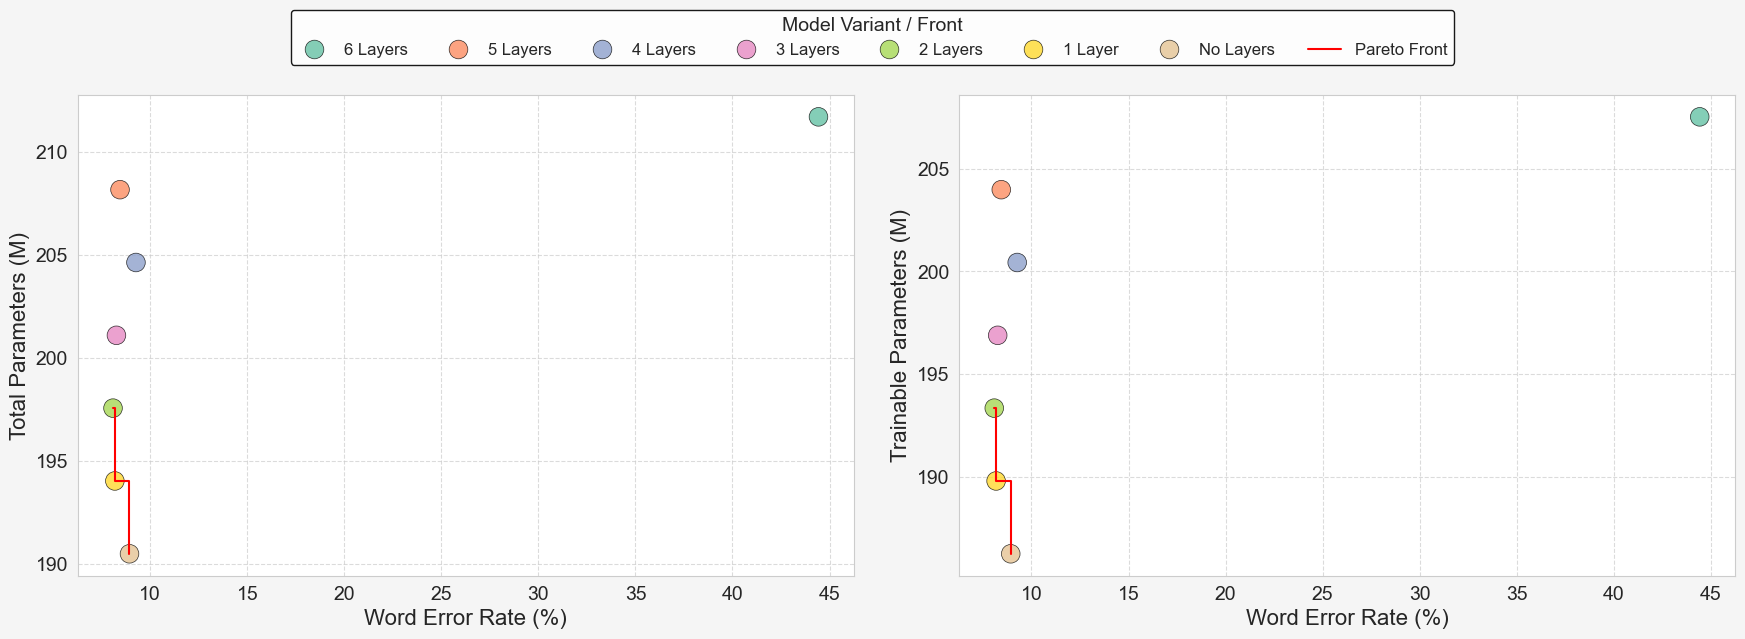
\includegraphics[width=1\textwidth]{obrazky-figures/plots/libri.png}
    \caption{Pareto front of total parameters/trainable parameters versus Word Error Rate (WER) for LibriSpeech.}
    \label{fig:pareto-front-librispeech}
\end{figure}

\begin{figure}[h!]
    \centering
    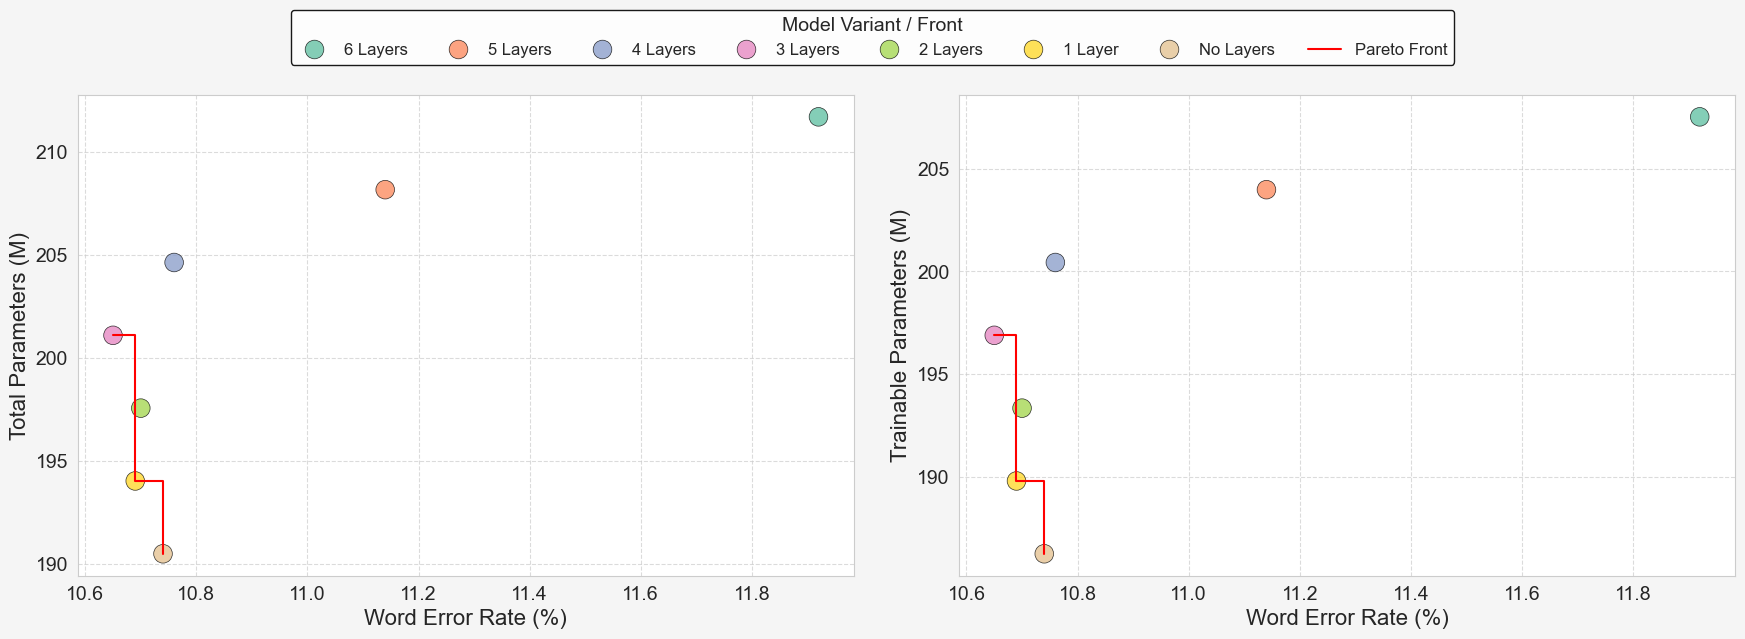
\includegraphics[width=1\textwidth]{obrazky-figures/plots/vox.png}
    \caption{Pareto front of total parameters/trainable parameters versus Word Error Rate (WER) for VoxPopuli.}
    \label{fig:pareto-front-voxpopuli}
\end{figure}


\begin{figure}[h]
    \centering
    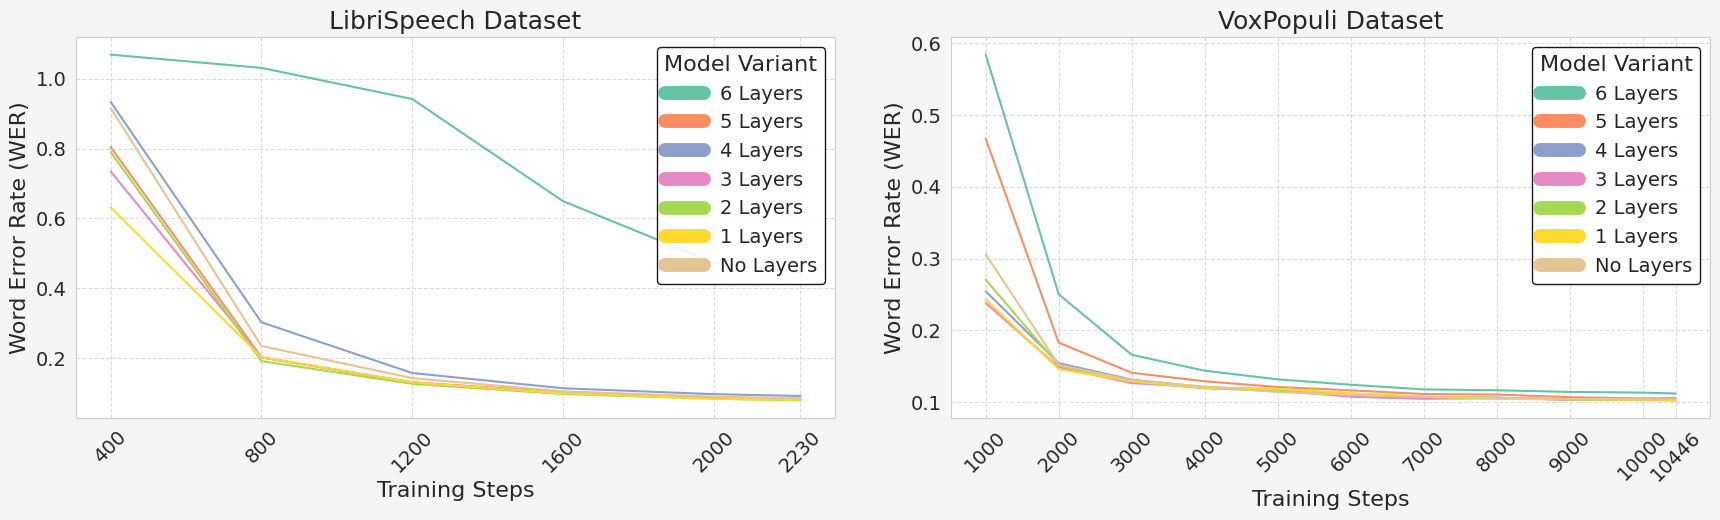
\includegraphics[width=1\textwidth]{obrazky-figures/plots/wer.png}
    \caption{Progression of WER on validation part for both datasets.}
    \label{fig:wer-progress-main}
\end{figure}


\begin{table}[h]
    \centering
    \begin{tabular}{@{} lcccccc @ {}}
    \toprule
    Adapters & Dev WER [\%] ↓ & Test WER [\%] ↓ & S & D & I & Adapter Params [M] \\
    \midrule
    0 & 8.5 & 8.9 & 7.3 & 0.7 & 1.0 & 0\\
    1 & 8.1 & 8.2 & 6.7 & 0.7 & 0.8 & 3.54\\
    2 & \textbf{7.9} & \textbf{8.1} & 6.6 & 0.6 & 0.9 & 7.08 \\
    3 & 8.3 & 8.6 & 6.9 & 0.6 & 0.8 & 10.6\\
    4 & 9.1 & 9.3 & 7.7 & 0.6 & 1.0 & 14.1\\
    5 & 8.3 & 8.4 & 6.9 & 0.6 & 0.9 & 17.7\\
    6 & 45 & 44 & 34 & 6.2 & 4.5 & 21.2\\
    \bottomrule
    \end{tabular}
    \caption{Effect of varying the number of convolutional adapter layers between the Wav2Vec2 encoder and BART decoder on ASR performance for the LibriSpeech (clean.100) dataset. Metrics include dev and test Word Error Rate (WER \%), test set error components (S, D, I), and the number of parameters in the adapter layers (M). The feature extractor is frozen. Numbers are rounded to 1 decimal place.}
    \label{tab:librispeech-wer-adapters}
\end{table}

\begin{table}[h]
    \centering
    \begin{tabular}{@{} lcccccc @ {}}
    \toprule
    Adapters & Dev WER [\%] ↓ & Test WER [\%] ↓ & S & D & I & Adapter Params [M] \\
    \midrule
    0 & 10.44 & 10.74 & 6.2 & 2.4 & 2.1 & 0 \\
    1 & 10.30 & 10.69 & 6.2 & 2.4 & 2.1 & 3.54 \\
    2 & 10.31 & 10.70 & 6.3 & 2.3 & 2.1 & 7.08 \\
    3 & 10.29 & \textbf{10.65} & 6.3 & 2.4 & 2.0 & 10.6 \\
    4 & \textbf{10.26} & 10.76 & 6.3 & 2.4 & 2.0 & 14.1 \\
    5 & 10.58 & 11.14 & 6.5 & 2.5 & 2.1 & 17.7\\
    6 & 11.21 & 11.92 & 7.0 & 2.6 & 2.2 & 21.2\\
    \bottomrule
    \end{tabular}
    \caption{Effect of varying the number of convolutional adapter layers between the Wav2Vec2 encoder and BART decoder on ASR performance for the VoxPopuli (English) dataset. Metrics include dev and test Word Error Rate (WER \%), test set error components (S, D, I), and the number of parameters in the adapter layers (M). The feature extractor is frozen.}
    \label{tab:voxpopuli-wer-adapters}
\end{table}

\begin{table}[h]
    \centering
    \begin{tabular}{@{}cc@{}}
    \toprule
         Number of Adapters &  Time [ms] ↓   \\
         \midrule
         0 & 49.4 ± 1 \\
         1 & 50.0 ± 1 \\
         2 & 48.1 ± 1 \\
         3 & 50.9 ± 1 \\
         4 & 50.7 ± 1  \\
         5 & 49.3 ± 1  \\
         6 & 49.7 ± 1 \\
    \bottomrule
    \end{tabular}
    \caption{Computational cost comparison: Average time per forward and backward pass (ms) for the Wav2Vec2-BART model with varying numbers of convolutional adapter layers (0 to 6). Measurements were taken on a representative ~10-second LibriSpeech audio sample.}
    \label{tab:conv_time}
\end{table}

\subsubsection{Conclusion}

The third experiment explores the impact of convolutional adapter layers in the Wav2Vec2 encoder of the encoder-decoder model. For LibriSpeech, 2 adapters yield the lowest WER, as shown in Table~\ref{tab:librispeech-wer-adapters}, but performance drops significantly with 6 adapters, likely due to over-compression because with 6 adapters, the sequence length gets 64-times shorter. For VoxPopuli, configurations with 1 to 4 adapters yield the best results.

WER progression (Figure~\ref{fig:wer-progress-main}) shows faster convergence with 1–3 adapters. Efficiency plots (Figures~\ref{fig:pareto-front-librispeech}, \ref{fig:pareto-front-voxpopuli}) reveal that more parameters do not mean the model will be linearly slower, that is because with more adapter layers the input length for the decoder becomes shorter. Time measurements reveal minimal variation in the average forward and backward pass time across different adapter configurations, ranging from 48.10ms to 50.90ms (Table \ref{tab:conv_time}). This indicates that adding convolutional adapter layers, within the tested range, has a negligible impact on processing speed. It's important to note that these measurements are specific to the utilized hardware and software environment, and different implementations or hardware might yield varying results, more details in Appendix \ref{app:timing-methodology}.

In summary, incorporating 1 to 3 adapter layers effectively improves performance by facilitating better alignment between the encoder and decoder representations. However, an excessive number of layers negatively impacts accuracy.


\section{Experimental Setup 4}
\label{experiment-3}

In the fourth experiment, I investigate the integration of Low-Rank Adaptation (LoRA) adapters \cite{hu2021lora} into the SpeechEncoderDecoder model to enhance parameter-efficient fine-tuning. Building on the findings from Experimental Setup~\ref{exp2actually} and Experimental Setup~\ref{exp2}, where three convolutional adapter layers are shown to be optimal for aligning the Wav2Vec2 encoder outputs with the BART decoder, this experiment aims to further reduce the computational resources of training, by using LoRA adapters. These adapters are applied to both the encoder and decoder, targeting key linear layers within the transformer architecture. Besides LoRA adapters, the convolutional adapters and the last linear layer (\texttt{lm\_head}) need to be trained.


\subsection{Experimental Design}

In this setup, LoRA adapters are applied to the linear layers within the attention and feed-forward blocks of both the Wav2Vec2 encoder and the BART decoder. These correspond to the query, key, value, and output projections in the multi-head attention mechanism, as well as the intermediate and output dense layers in the feed-forward networks. The number of trainable LoRA parameters depends on the chosen rank value. 

In addition to the LoRA adapters, the convolutional adapter layers (10.6M parameters) and the \texttt{lm\_head} (38.6M parameters) are trained. Together, these two components dominate the trainable parameter count and comprise roughly 25\% of the total parameters in the model.

For the initial LoRA experiments, I focus on varying the rank \( r \) and the scaling factor \( \alpha \). For \( \alpha \) value, I explore values that are significantly higher than commonly used heuristics (e.g., $\alpha = r$ or $\alpha = 2r$). The rationale is to investigate whether a stronger adaptation signal, achieved by increasing the magnitude of the LoRA update ($\frac{\alpha}{r} \cdot BA$), is necessary to effectively fine-tune the pre-trained model for the ASR task. This approach aims to potentially achieve a lower Word Error Rate by allowing for more substantial deviations from the original weights. However, this choice risks training instability, as large \( \alpha / r \) ratios amplify gradient updates to the effective weights, potentially leading to divergence and training instability.

\subsubsection{Training Details}

The training configuration mirrors that of Experimental Setup 2; only thing that changed was the number of epochs on the VoxPopuli \cite{wang2021voxpopulilargescalemultilingualspeech} dataset from 6 to 5. I made this decision since I have not seen much improvement in training for longer, and also, in some cases, the model got worse.

Performance is evaluated using the same approach as in previous experiments, with results reported in Tables~\ref{tab:librispeech-lora} and~\ref{tab:voxpopuli-lora}. These tables include the LoRA trainable parameters (excluding convolutional adapters and \texttt{lm\_head}) alongside WER for each configuration. Computational efficiency is measured the exact same way as in previous experiment \ref{exp2} and is summarized in Table~\ref{tab:loras_time}. Figures~\ref{fig:pareto-front-librispeech_lora} and ~\ref{fig:pareto-front-voxpopuli_lora} show the trade-off between different LoRA configurations, visualized as Pareto fronts.

\begin{table}[h]
    \centering
    \begin{tabular}{@{} cccccccc @ {}}
        \toprule
        Rank & Alpha & Dev WER [\%] \(\downarrow\) & Test WER [\%] \(\downarrow\) & S & D & I & LoRA Params [M] \\
        \midrule
        Full FT & — & 8.29 & 8.26 & 6.9 & 0.6 & 0.8 & — \\
        \midrule
        \multirow{5}{*}{16} & 128 & 10.4 & 10.7 & 8.7 & 0.9 & 1.0 & \multirow{5}{*}{4.6} \\
        & 192 & 10.2 & 10.5 & 8.7 & 0.8 & 1.1 & \\
        & 256 & 10.4 & 10.5 & 8.8 & 0.8 & 1.0 & \\
        & 384 & 10.5 & 10.9 & 8.8 & 1.1 & 1.0 & \\
        & 512 & 158 & 161 & 82.1 & 9.5 & 70.4 & \\
        \midrule[0.5pt]
        \multirow{5}{*}{32} & 128 & 10.1 & 10.2 & 8.3 & 0.9 & 1.0 & \multirow{5}{*}{9.1} \\
        & 192 & 9.8 & 9.9 & 8.2 & 0.8 & 1.0 & \\
        & 256 & 9.4 & 9.6 & 8.0 & 0.6 & 1.0 & \\
        & 384 & 9.6 & 9.6 & 8.0 & 0.6 & 1.0 & \\
        & 512 & 9.6 & 9.8 & 8.3 & 0.6 & 1.0 & \\
        \midrule[0.5pt]
        \multirow{5}{*}{64} & 128 & 9.7 & 9.9 & 8.1 & 0.8 & 1.0 & \multirow{5}{*}{18.3} \\
        & 192 & 9.3 & 9.4 & 7.7 & 0.7 & 0.9 & \\
        & 256 & 9.4 & 9.5 & 7.8 & 0.7 & 1.0 & \\
        & 384 & 9.0 & 9.0 & 7.5 & 0.6 & 0.9 & \\
        & 512 & 9.1 & 9.2 & 7.6 & 0.7 & 0.9 & \\
        \midrule[0.5pt]
        \multirow{5}{*}{128} & 128 & 9.4 & 9.8 & 8.0 & 0.8 & 1.0 & \multirow{5}{*}{36.6} \\
        & 192 & 9.1 & 9.2 & 7.7 & 0.6 & 0.9 & \\
        & 256 & 8.9 & 9.1 & 7.5 & 0.8 & 0.9 & \\
        & 384 & 8.8 & 9.0 & 7.4 & 0.7 & 0.9 & \\
        & 512 & \textbf{8.6} & \textbf{8.7} & 7.2 & 0.7 & 0.8 & \\
        \bottomrule
    \end{tabular}
    \caption{Performance evaluation of Low-Rank Adaptation (LoRA) for fine-tuning the Wav2Vec2-BART ASR model on LibriSpeech (clean.100), varying rank (\( r \)) and alpha (\( \alpha \)) values. The model includes 3 convolutional adapters and a frozen feature extractor. Metrics include dev and test WER (\%), error components (S, D, I), and number of LoRA-specific parameters (M). The full fine-tuning (Full FT) baseline with 3 adapters is included for comparison. Numbers are rounded to 1 decimal place.}
    \label{tab:librispeech-lora}
\end{table}

\begin{table}[h]
    \centering
    \begin{tabular}{@{} cccccccc @ {}}
        \toprule
        Rank & Alpha & Dev WER [\%] \(\downarrow\) & Test WER [\%] \(\downarrow\) & S & D & I & LoRA Params [M] \\
        \midrule
        Full FT & — & 10.29 & 10.65 & 6.3 & 2.4 & 2.0 & — \\
        \midrule
        \multirow{5}{*}{16} & 128 & 12.9 & 13.5 & 8.2 & 2.8 & 2.5 &
        \multirow{5}{*}{4.6} \\
        & 192 & 16.1 & 16.4 & 8.6 & 5.4 & 2.4 & \\
        & 256 & 12.6 & 12.9 & 7.9 & 2.5 & 2.4  \\
        & 384 & 12.3 & 12.8 & 7.7 & 2.8 & 2.2 & \\
        & 512 & 12.7 & 13.1 & 7.9 & 2.8 & 2.4 \\
        \midrule[0.5pt]
        \multirow{5}{*}{32} & 128 & 12.5 & 13.2 & 7.9 & 2.9 & 2.5 & 
        \multirow{5}{*}{9.1} \\
        & 192 & 12.3 & 12.8 & 7.7 & 2.7 & 2.4 & \\
        & 256 & 12.9 & 13.6 & 8.1 & 3.1 & 2.3  \\
        & 384 & 11.7 & 12.3 & 7.5 & 2.5 & 2.3 & \\
        & 512 & 11.6 & 12.2 & 7.4 & 2.5 & 2.3 \\
        \midrule[0.5pt]
        \multirow{5}{*}{64} & 128 & 13.1 & 13.6 & 8.1 & 3.0 & 2.4 & 
        \multirow{5}{*}{18.3} \\
        & 192 & 12.1 & 12.7 & 7.6 & 2.6 & 2.4 & \\
        & 256 & 11.9 & 12.4 & 7.6 & 2.5 & 2.3 \\
        & 384 & 11.6 & 12.0 & 7.2 & 2.5 & 2.3 & \\
        & 512 & 11.7 & \textbf{11.9} & 7.2 & 2.5 & 2.1 \\
        \midrule[0.5pt]
        \multirow{5}{*}{128} & 128 & 16.4 & 16.7 & 9.2 & 4.5 & 3.1 & 
        \multirow{5}{*}{36.6} \\
        & 192 & 11.9 & 12.7 & 7.7 & 2.6 & 2.5 & \\
        & 256 & 11.7 & 12.5 & 7.5 & 2.6 & 2.4  \\
        & 384 & \textbf{11.3} & 12.1 & 7.3 & 2.5 & 2.3 & \\
        & 512 & 12.1 & 12.5 & 7.4 & 2.8 & 2.3  \\
        \bottomrule
    \end{tabular}
    \caption{Performance evaluation of Low-Rank Adaptation (LoRA) for fine-tuning the Wav2Vec2-BART ASR model on VoxPopuli (English), varying rank (\( r \)) and alpha (\( \alpha \)) values. The model includes 3 convolutional adapters and a frozen feature extractor. Metrics include dev and test WER (\%), error components (S, D, I), and number of LoRA-specific parameters (M). The full fine-tuning (Full FT) baseline with 3 adapters is included for comparison. Numbers are rounded to 1 decimal place.}
    \label{tab:voxpopuli-lora}
\end{table}

\begin{table}[h]
    \centering
    \begin{tabular}{@{}cc@{}}
    \toprule
        Rank &  Time [ms] ↓   \\
         \midrule
         16 & 101 ± 2 \\
         32 & 101 ± 2 \\
         64 & 103 ± 3 \\
         128 & 102 ± 3 \\
    \bottomrule
    \end{tabular}
    \caption{Computational cost comparison: Average time per forward and backward pass (ms) for the Wav2Vec2-BART model using LoRA adapters with varying ranks (\( r \)). Measurements were taken on a representative ~10-second LibriSpeech audio sample.}
    \label{tab:loras_time}
\end{table}

\begin{figure}[h!]
    \centering
    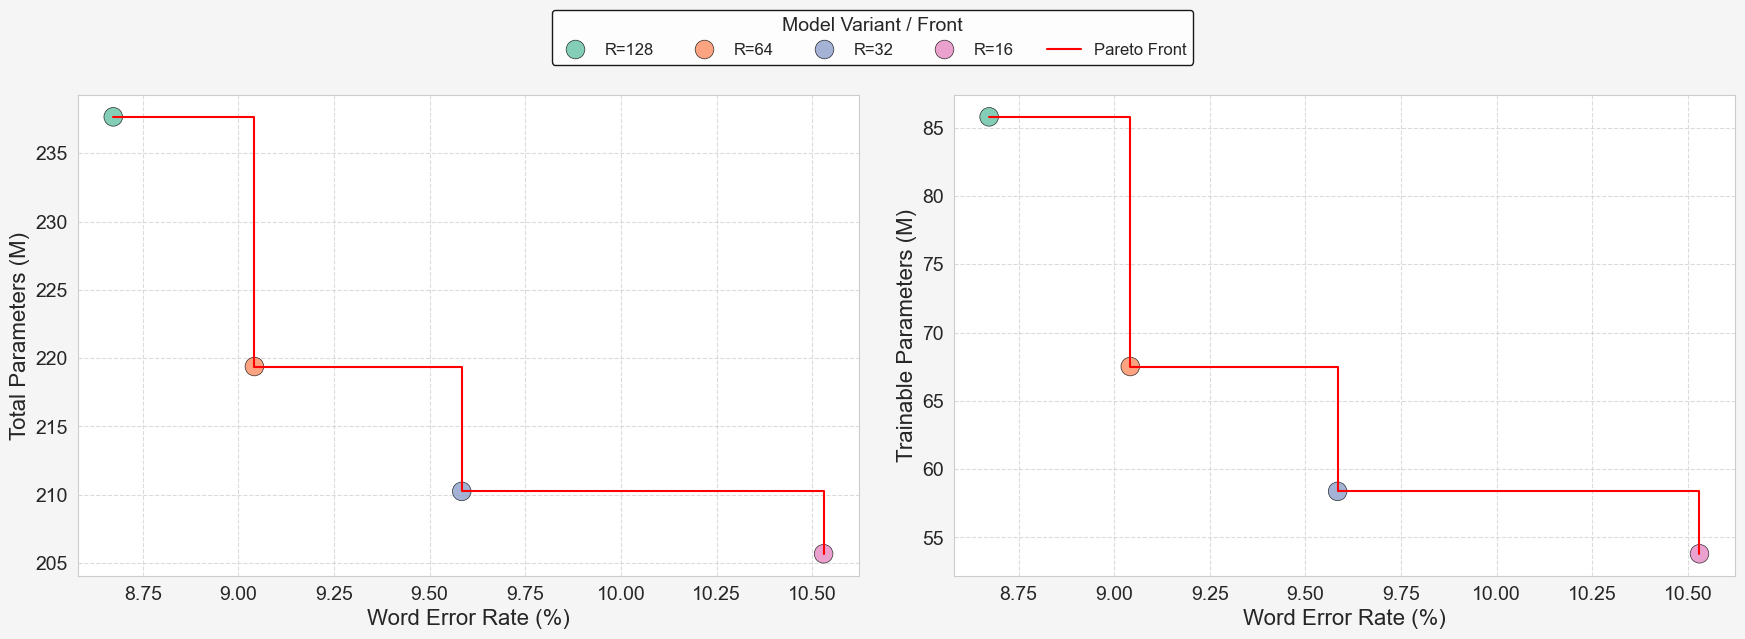
\includegraphics[width=1\textwidth]{obrazky-figures/plots/libri_lora.png}
    \caption{Pareto front of total parameters/trainable parameters versus Word Error Rate for LibriSpeech on circa 10 seconds long sample for different LoRA configurations.}
    \label{fig:pareto-front-librispeech_lora}
\end{figure}

\begin{figure}[h!]
    \centering
    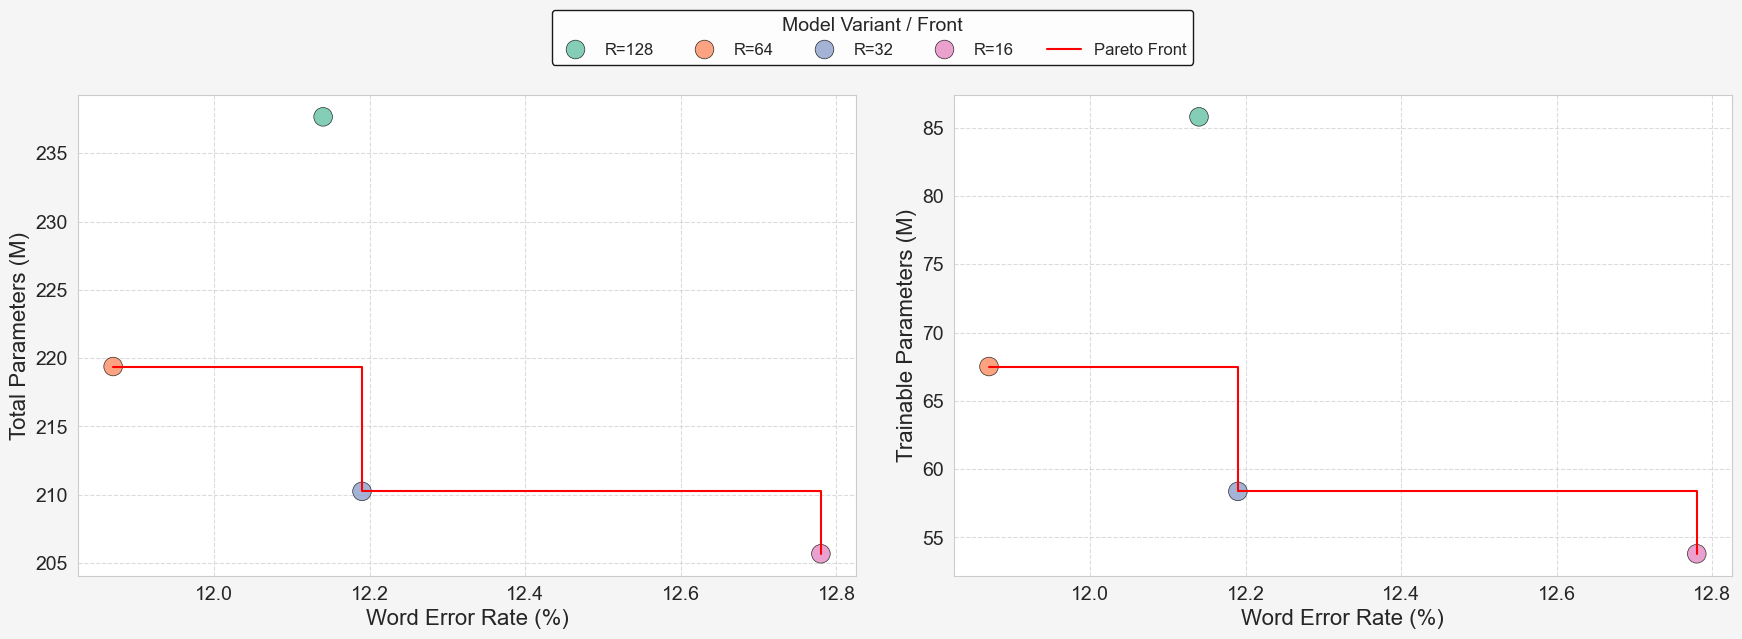
\includegraphics[width=1\textwidth]{obrazky-figures/plots/vox_lora.png}
    \caption{Pareto front of total parameters/trainable parameters versus Word Error Rate for VoxPopuli on circa 10 seconds long sample for different LoRA configurations.}
    \label{fig:pareto-front-voxpopuli_lora}
\end{figure}


\subsubsection{Conclusion}

LoRA proves effective for parameter-efficient fine-tuning in this setup. An increase in the rank $r$ consistently leads to improved performance, as indicated by a reduction in the WER. This improvement is attributed to the fact that a higher rank allows the LoRA layers more degrees of freedom to adapt the original weights.


The scaling factor \( \alpha \) has a more complex effect. I used high \( \alpha \) values to try to get the best WER, but very high \( \alpha \) (like 512 with $r$=16 on LibriSpeech) made training unstable. From the results, we see that the best LoRA setup is different for each dataset.

LoRA uses many fewer trainable parameters than fine-tuning the whole model. Even the biggest LoRA setup (\( r \)=128) adds only 36.6M parameters. Adding the convolutional adapters (10.6M) and \texttt{ lm\_head} (38.6M), the total count is still much smaller than the full fine-tuning. Table~\ref{tab:loras_time} shows that changing the LoRA rank doesn't change the training time much (101-103ms per forward and backward pass).

The Pareto fronts (Figures \ref{fig:pareto-front-librispeech_lora} and \ref{fig:pareto-front-voxpopuli_lora}) show the trade-off between parameters and WER. Choosing the right rank and alpha gives good performance without adding many parameters. Compared to Experiment~\label{exp2actually}, LoRA had slightly worse performance on LibriSpeech and on VoxPopuli. The focus was on using few resources, not just getting the absolute best WER.

In short, LoRA is good for fine-tuning this encoder-decoder model because it reduces parameters a lot while keeping good performance. It is important to say that this parameter efficiency becomes even more advantageous for larger sized models, where the number of parameters added by LoRA is much smaller relative to the total model size. The best settings depend on the dataset. The training time stays about the same for different ranks but are ~2 times slower than full-finetuing.

\section{Experimental Setup 5}
In the fifth experiment, I use Weight-Decomposed Low-Rank Adaptation (DoRA) \cite{liu2024dora}, which is a modified version of LoRA. This experiment continues to use the optimal configuration identified in Experimental Setup~\ref{exp2actually} and~\ref{exp2}, which includes three convolutional adapter layers and frozen feature extractor.


In this experimental setup, DoRA adapters are applied to the same linear layers within the Wav2Vec2 encoder and BART decoder as in Experimental Setup~\ref{experiment-3}. I vary the rank \( r \) and \( \alpha \) values for the LoRA component within DoRA.  The number of trainable parameters in DoRA will be slightly higher than in the corresponding LoRA configurations due to the inclusion of the trainable magnitude vector \( m \). For each linear layer with a weight matrix of size \( d \times k \), the magnitude vector introduces an additional \( k \) trainable parameters.

The training details, including optimizer (AdamW), learning rate scheduler, batch sizes, and gradient accumulation, are identical to those used in Experimental Setup~\ref{experiment-3}.  Performance is evaluated using Word Error Rate (WER). Computational efficiency is measured using the average time per forward and backward pass. The measurements are summarized in Table~\ref{tab:doras_time}.

\begin{table}[h]
    \centering
    \begin{tabular}{@{} cccccccc @ {}}
        \toprule
        Rank & Alpha & Dev WER [\%] \(\downarrow\) & Test WER [\%] \(\downarrow\) & S & D & I & DoRA Params [M] \\
        \midrule
        Full FT & — & 8.29 & 8.26 & 6.9 & 0.6 & 0.8 & — \\
        \midrule
        \multirow{3}{*}{16} & 256 & 10.1 & 10.2 & 8.3 & 0.9 & 1.0 & \multirow{3}{*}{4.7} \\
        & 384 & 10.4 & 10.5 & 8.6 & 0.9 & 1.0 &  \\
        & 512 & 10.4 & 10.6 & 8.7 & 0.8 & 1.1 & \\
        \midrule[0.5pt]
        \multirow{3}{*}{32} & 256 & 9.6 & 9.7 & 8.0 & 0.8 & 0.9 & \multirow{3}{*}{9.3} \\
        & 384 & 9.5 & 9.6 & 7.9 & 0.7 & 1.0 & \\
        & 512 & 9.5 & 9.5 & 7.8 & 0.8 & 0.9 & \\
        \midrule[0.5pt]
         \multirow{3}{*}{64} & 256 & 9.1 & 9.1 & 7.5 & 0.6 & 0.9 & \multirow{3}{*}{18.4} \\
        & 384 & 9.2 & 9.2 & 7.6 & 0.7 & 0.9 &  \\
        & 512 & 196 & 201 & 82 & 4.6 & 113 & \\
        \midrule[0.5pt]
        \multirow{3}{*}{128} & 256 & 9.0 & 9.1 & 7.5 & 0.8 & 0.8 & \multirow{3}{*}{36.7} \\
        & 384 & 8.9 & 9.1 & 7.4 & 0.8 & 0.9 & \\
        & 512 & \textbf{8.7} & \textbf{8.9} & 7.3 & 0.7 & 0.9 & \\
        \bottomrule
    \end{tabular}
    \caption{Performance evaluation of Weight-Decomposed Low-Rank Adaptation (DoRA) for fine-tuning the Wav2Vec2-BART ASR model on LibriSpeech (clean.100), varying rank (\( r \)) and alpha (\( \alpha \)) values. The model includes 3 convolutional adapters and a frozen feature extractor. Metrics include dev and test WER (\%), error components (S, D, I), and number of DoRA-specific parameters (M). The full fine-tuning (Full FT) baseline with 3 adapters is included for comparison. Numbers are rounded to 1 decimal place.}
    \label{tab:librispeech-dora}
\end{table}

\begin{table}[h]
    \centering
    \begin{tabular}{@{} cccccccc @ {}}
        \toprule
        Rank & Alpha & Dev WER [\%] \(\downarrow\) & Test WER [\%] \(\downarrow\) & S & D & I & DoRA Params [M] \\
        \midrule
        Full FT & — & 10.3 & 10.7 & 6.3 & 2.4 & 2.0 & — \\
        \midrule
        \multirow{3}{*}{16} & 256 & 12.3 & 12.9 & 7.9 & 2.5 & 2.4 & \multirow{3}{*}{4.7} \\
        & 384 & 12.0 & 12.4 & 7.5 & 2.7 & 2.3 & \\
        & 512 & 12.5 & 12.9 & 7.6 & 3.0 & 2.3 & \\
        \midrule[0.5pt]
        \multirow{3}{*}{32}  & 256 & 12.6 & 13.2 & 8.0 & 2.7 & 2.5 & \multirow{3}{*}{9.3} \\
        & 384 & 11.9 & 12.5 & 7.4 & 2.8 & 2.3 & \\
        & 512 & 11.6 & 12.0 & 7.2 & 2.5 & 2.3 & \\
        \midrule[0.5pt]
        \multirow{3}{*}{64} & 256 & 11.9 & 12.4 & 7.4 & 2.6 & 2.3 & \multirow{3}{*}{18.4} \\
        & 384 & 12.9 & 13.4 & 7.8 & 3.0 & 2.5 & \\
        & 512 & \textbf{11.4} & \textbf{11.9} & 7.1 & 2.7 & 2.2 & \\
        \midrule[0.5pt]
        \multirow{3}{*}{128} & 256 & 12.5 & 13.3 & 7.7 & 3.2 & 2.4 & \multirow{3}{*}{36.7} \\
        & 384 & 11.9 & 12.4 & 7.3 & 2.7 & 2.4 & \\
        & 512 & 12.6 & 12.8 & 7.4 & 3.1 & 2.3 & \\
        \bottomrule
    \end{tabular}
    \caption{Performance evaluation of Weight-Decomposed Low-Rank Adaptation (DoRA) for fine-tuning the Wav2Vec2-BART ASR model on VoxPopuli (English), varying rank (\( r \)) and alpha (\( \alpha \)) values. The model includes 3 convolutional adapters and a frozen feature extractor. Metrics include dev and test WER (\%), error components (S, D, I), and number of DoRA-specific parameters (M). The full fine-tuning (Full FT) baseline with 3 adapters is included for comparison. Numbers are rounded to 1 decimal place.}
    \label{tab:voxpopuli-dora}
\end{table}

\begin{table}[h]
    \centering
    \begin{tabular}{@{}cc@{}}
    \toprule
        Rank &  Time [ms] ↓   \\
         \midrule
         16 & 184 ± 3 \\
         32 & 181 ± 4 \\
         64 & 185 ± 3 \\
         128 & 184 ± 4 \\
    \bottomrule
    \end{tabular}
    \caption{Computational cost comparison: Average time per forward and backward pass (ms) for the Wav2Vec2-BART model using DoRA adapters with varying ranks (\( r \)). Measurements were taken on a representative ~10-second LibriSpeech audio sample.}
    \label{tab:doras_time}
\end{table}

\begin{figure}[h!]
    \centering
    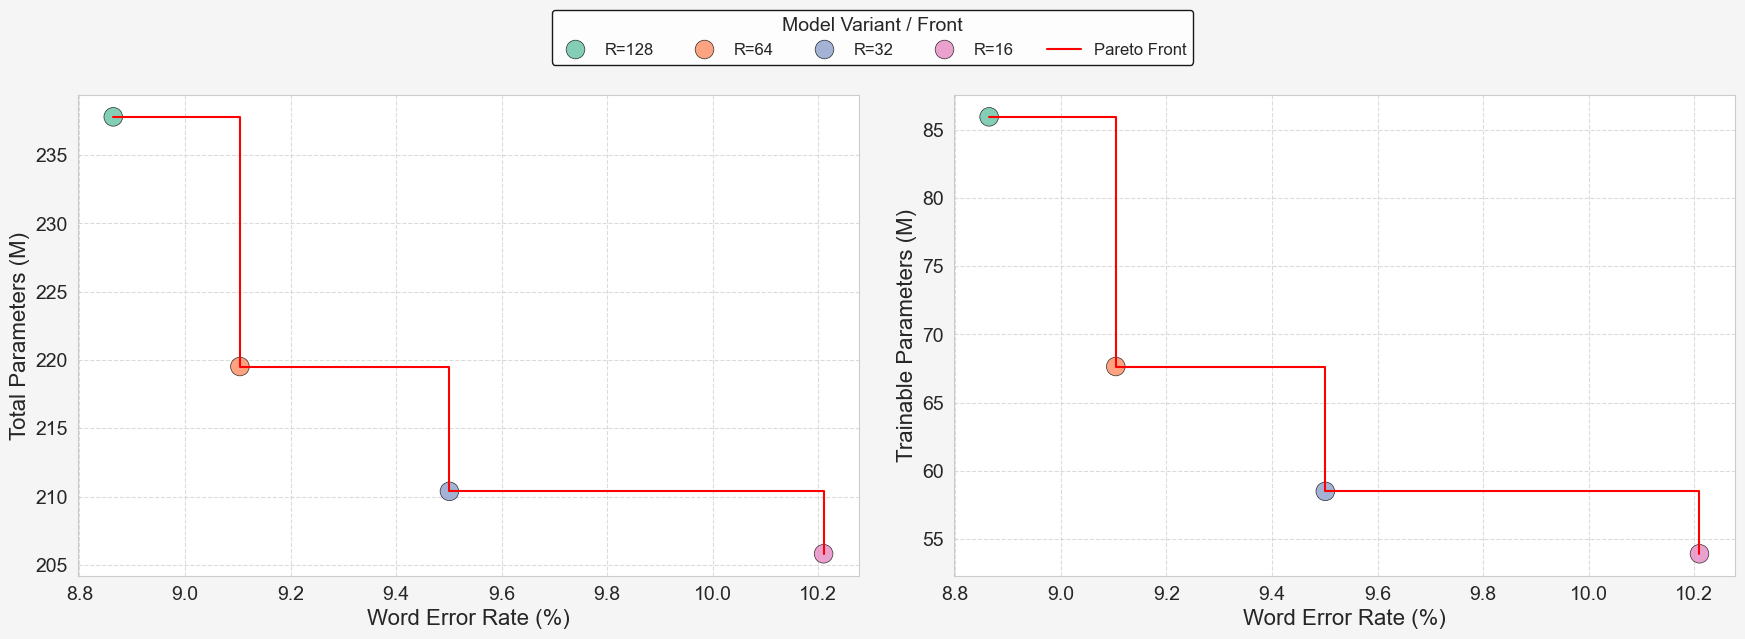
\includegraphics[width=1\textwidth]{obrazky-figures/plots/libri_dora.png} 
    \caption{Pareto front of total parameters/trainable parameters versus Word Error Rate for LibriSpeech on a circa 10-second long sample for different DoRA configurations.}
    \label{fig:pareto-front-librispeech-dora}
\end{figure}

\begin{figure}[h!]
    \centering
    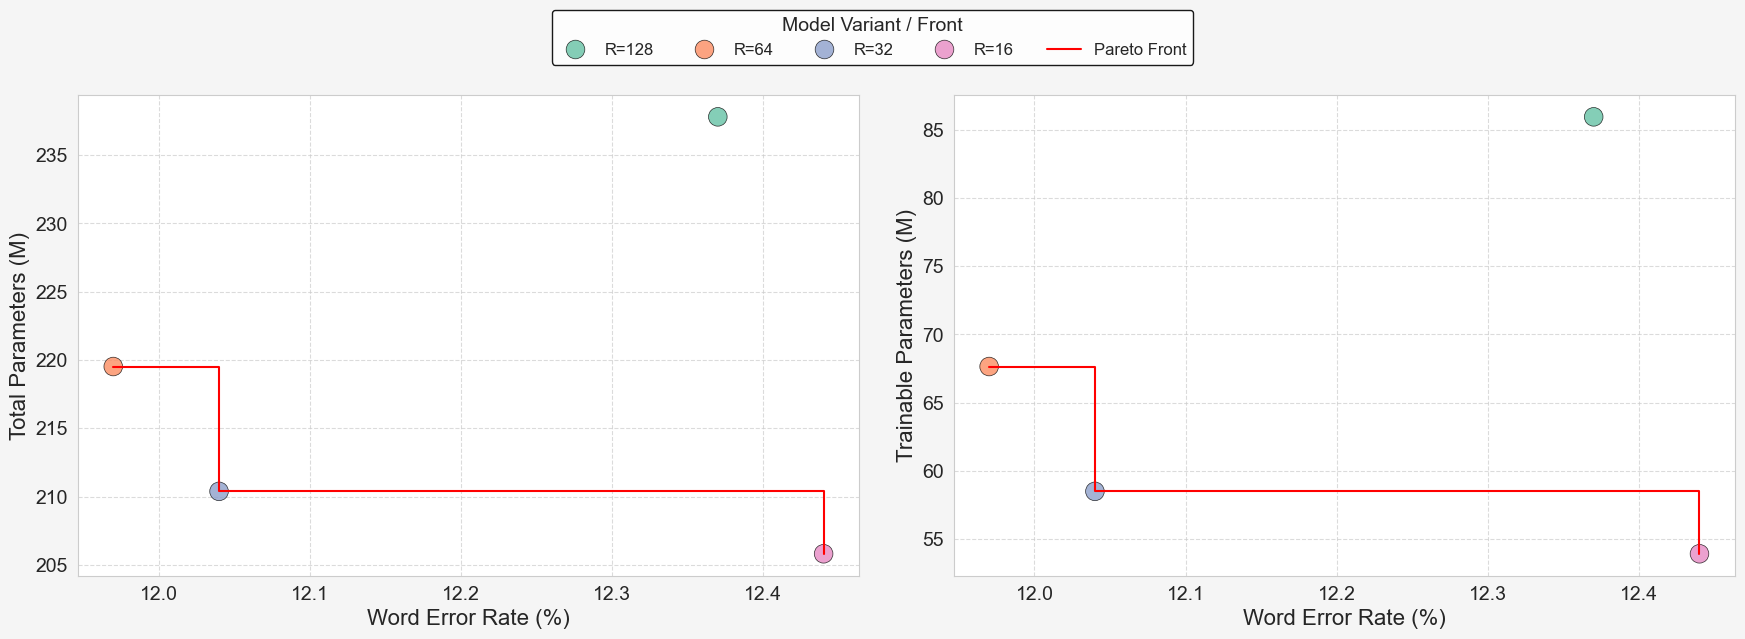
\includegraphics[width=1\textwidth]{obrazky-figures/plots/vox_dora.png} 
    \caption{Pareto front of total parameters/trainable parameters versus Word Error Rate for VoxPopuli on a circa 10-second long sample for different DoRA configurations.}
    \label{fig:pareto-front-voxpopuli-dora}
\end{figure}

\subsubsection{Conclusion}

The DoRA experiments evaluate an alternative parameter-efficient fine-tuning technique that tries to enhance LoRA. Comparing these results to those from Experimental Setup~\ref{experiment-3} in order to assess DoRA's relative effectiveness in this task.

Similar to LoRA, increasing the rank \( r \) within DoRA generally tends to improve performance (lower WER), although this trend is not perfectly consistent, particularly on the VoxPopuli dataset (Table \ref{tab:voxpopuli-dora}). The scaling factor \( \alpha \) continues to show a complex relationship with performance, with higher values often yielding better results but also increasing the risk of training instability, as seen with the \( r=64, \alpha=512 \) configuration on LibriSpeech (Table \ref{tab:librispeech-dora}). In terms of absolute performance, the best DoRA configurations achieved slightly higher WER compared to the best LoRA configurations on both datasets.

Regarding parameter efficiency, DoRA introduces a marginal increase in trainable parameters compared to LoRA due to the addition of the magnitude vector \( m \). For instance, with \( r=128 \), DoRA adds 36.7M parameters compared to LoRA's 36.6M. DoRA maintains a similar high level of parameter efficiency as LoRA compared to full fine-tuning.

A significant difference emerges in computational cost. Table \ref{tab:doras_time} shows that the average time per forward and backward pass for DoRA ranges from 181ms to 185ms, irrespective of rank. This is substantially slower than LoRA, which ranged from 101ms to 103ms, representing an approximate $ 80\% $ increase in step time. Compared to full fine-tuning (~51ms from Table \ref{tab:conv_time}), DoRA is about 3.6 times slower per step. This overhead comes from the additional computations involved in the weight decomposition and normalization specific to DoRA.

\section{Experimental Setup 6}
\label{exp:voxpopuli_pretrained_encoders_and_decoder}

This sixth experiment investigates the influence of encoder's and decoder's pre-training data domain strategies on downstream ASR performance, specifically when targeting the VoxPopuli dataset because the pre-trained wav2vec2 base model includes LibriSpeech in its pre-training 
The hypothesis is that domain-specific encoder pre-training or decoder continuous pre-training might provide better initialization and lead to improved performance when fine-tuning the full encoder-decoder model on the labeled VoxPopuli English subset.

\subsection{Experimental Design: Encoder Pre-training}
This part of the experiment builds directly upon the optimal configuration identified in previous setups. The only variable changed here is the specific pre-trained checkpoint used to initialize the Wav2Vec2 encoder component. I use Wav2Vec2 checkpoints pre-trained on varying amounts and subsets of the VoxPopuli corpus. The following checkpoints are evaluated:
\begin{itemize}
    \item \texttt{facebook/wav2vec2-base-en-voxpopuli-v2}: Pre-trained on 24.1k hours of unlabeled English VoxPopuli data.
    \item \texttt{facebook/wav2vec2-base-10k-voxpopuli-ft-en}: Pre-trained on 10k hours of unlabeled VoxPopuli, then fine-tuned on labeled English VoxPopuli dataset.
    \item \texttt{facebook/wav2vec2-base-100k-voxpopuli}: Pre-trained on 100k hours of unlabeled multilingual VoxPopuli data.
    \item \texttt{facebook/wav2vec2-base-10k-voxpopuli}: Pre-trained on 10k hours of unlabeled multilingual VoxPopuli data.
\end{itemize}
The performance of these models is compared against the baseline model from Experimental Setup~\ref{exp2} when trained and evaluated on the VoxPopuli English dataset. The models are trained exclusively on the VoxPopuli (English) dataset using the same training framework detailed in Section~\ref{sec:common_training_details}.

\subsection{Experimental Design: Decoder Continuous Pre-training}
For this part of the experiment, I apply additional pre-training steps to the decoder, using the VoxPopuli English training text data. The goal is to adapt the decoder to the target domain's linguistic style using self-supervised objectives similar to the original paper \cite{lewis2019bartdenoisingsequencetosequencepretraining}. Since the original BART pre-training recipe wasn't fully detailed by Facebook, I use and compare two common strategies based on their paper and available code examples:

\begin{itemize}
    \item \textbf{Text Infilling}: This objective aims to teach the model to predict missing text spans. Spans of text are sampled (lengths drawn from a Poisson distribution, $\lambda=3.0$), and each chosen span is replaced by a single \texttt{[MASK]} token. The decoder is trained to reconstruct the original, uncorrupted text sequence. This differs slightly from some interpretations where multiple mask tokens might be used, but captures the core idea of predicting variable-length missing content.
    \item \textbf{Denoising + Sentence Permutation}: This objective combines text infilling with sentence-level shuffling, mimicking the combination reported in the original BART paper. It involves:
        \begin{enumerate}
            \item \textit{Sentence Permutation}: Documents are segmented into sentences (based on \texttt{EOS} tokens), and the order of these sentences is randomly shuffled with a certain probability.
            \item \textit{Text Infilling}: Similar to the above, text spans/whole words are masked based on a mask ratio (\texttt{mask\_ratio=0.15}) and Poisson-sampled lengths ($\lambda=3.0$), are replaced by \texttt{[MASK]} tokens. The decoder must reconstruct the original text from this doubly corrupted input.
        \end{enumerate}
\end{itemize}
These decoder pre-training steps were performed on the VoxPopuli English text data. Both are continuously pre-trained on additional 500 epochs on training data.

\subsection{Results and Analysis}
The performance results for each encoder and decoder pre-training configuration are presented in Table~\ref{tab:voxpopuli_pretrained_encoders_decoder_results}. The table includes the Word Error Rate (WER) and its components (substitutions, deletions, insertions) for the VoxPopuli English test set.

\begin{table}[h]
    \centering
    \begin{tabular}{@{} lcccccc @ {}}
    \toprule
    Pre-training Configuration & Dev WER [\%] ↓ & Test WER [\%] ↓ & S & D & I \\
    \midrule
    Baseline ( 53k h) & 10.29 & 10.65 & 6.3 & 2.4 & 2.0 \\
    \midrule
    \multicolumn{6}{l}{\textit{Encoder Pre-training Variations}} \\
     
     VoxPopuli EN (24.1k h) & 9.20 & 9.88 & 5.6 & 2.2 & 2.1 \\
     VoxPopuli (10k h) + FT EN  & 10.55 & 10.88 & 6.5 & 2.3 & 2.1 \\
     VoxPopuli Multi (100k h) & 10.62 & 11.22 & 6.8 & 2.4 & 2.0 \\
     VoxPopuli Multi (10k h) & 11.15 & 12.03 & 7.2 & 2.5 & 2.3 \\
    \midrule
    \multicolumn{6}{l}{\textit{Decoder Continuous Pre-training}} \\
     Text Infilling & 10.26 & 10.71 & 6.4 & 2.3 & 2.1 \\
     Denoising + Sent. Perm. & 10.21 & 10.80 & 6.4 & 2.3 & 2.1 \\
    \bottomrule
    \end{tabular}
    \caption{Impact of varying encoder pre-training data domain and decoder continuous pre-training strategy on ASR performance on the VoxPopuli (English) dataset. Compares different Wav2Vec2 encoder checkpoints and two BART decoder pre-training objectives against the baseline model (3 adapters, frozen feature extractor). Metrics include dev and test WER (\%), and test set error components (S, D, I).}
    \label{tab:voxpopuli_pretrained_encoders_decoder_results}
\end{table}


\subsubsection{Conclusion}
For the encoder, the results reveal a significant benefit from domain-specific pre-training. The Wav2Vec2 encoder pre-trained specifically on English VoxPopuli data achieves the lowest WER (9.88\% test), substantially outperforming the standard \texttt{wav2vec2-base} baseline (10.65\% test). This indicates that aligning the encoder's pre-training data domain and language with the target task provides a considerable advantage. Notably, other VoxPopuli-based encoders, including those pre-trained on multilingual data or incorporating fine-tuning, did not surpass the baseline performance.

Conversely, for the decoder, applying continuous pre-training on domain-specific data using BART-inspired objectives does not yield improvements. Both the Text Infilling (10.71\% test WER) and the Denoising + Sentence Permutation (10.80\% test WER) strategies resulted in slightly higher error rates compared to the baseline model. The variance in the results does not show any difference from the baseline and is not significant enough. In this setup, adapting the pre-trained BART decoder further using self-supervised objectives on the target text domain does not show that it should increase the performance of encoder decoder for ASR task.

These experiments utilize a fixed set of fine-tuning hyperparameters based on the baseline model. The optimal hyperparameters might differ for each pre-trained encoder and decoder checkpoint. Specific hyperparameter tuning for each checkpoint might yield different performance results.


\section{Experimental Setup 7}
\label{exp:ctc_comparison}

This final experiment aims to compare the performance of the encoder-decoder model against a Connectionist Temporal Classification (CTC) based model. CTC is explained in section \ref{ctc_theory}.

\subsection{CTC Model Configuration}
The CTC model uses the same pre-trained Wav2Vec2-base encoder, which is used with the previous experiments for the encoder-decoder model. The CTC model architecture uses a standard CTC setup where a linear classification head is added directly on top of the Wav2Vec2 encoder's output sequence. This head projects the encoder's final hidden states into logit vectors, where the dimension of each vector corresponds to the size of the target vocabulary.

A difference from the encoder-decoder setup is also in the vocabulary construction. Rather than using the large BART vocabulary, a much smaller vocabulary is created specifically for each dataset based on the characters present in their training transcriptions. This involves extracting all unique characters from the target text, sorting them, and assigning unique integer IDs. Special tokens are included: a padding token, an unknown token, and a word delimiter token (used to represent spaces). 

Consistent with the findings from Experiment~\ref{exp2actually}, the Wav2Vec2 feature extractor layers are kept frozen during training. 

\subsection{Training Details}
The CTC models are trained using CTC loss function. Standard optimization techniques are used, including the AdamW optimizer and a learning rate scheduler. The training parameters for the CTC models (such as learning rate, number of epochs, and scheduler details) are determined empirically. A few training runs are conducted for each dataset to identify settings that yield reasonable convergence and representative performance for the CTC architecture on the given task.

\subsection{Results and Analysis}
The performance comparison between the CTC model and the baseline encoder-decoder model on both datasets is presented in Table~\ref{tab:ctc_vs_encdec_results}.

\begin{table}[h]
    \centering
    \begin{tabular}{@{} l l ccccc @ {}}
    \toprule
    Dataset & Model & Dev WER [\%] ↓ & Test WER [\%] ↓ & S & D & I  \\
    \midrule
    \multirow{2}{*}{LibriSpeech}
        & Encoder-decoder & 8.29 & 8.26 & 6.9 & 0.6 & 0.8 \\ % From Table 7
        & CTC & 11.87 & 11.87 & 5.7 & 0.4 & 5.8 \\
    \midrule
    \multirow{2}{*}{VoxPopuli}
        & Encoder-decoder & 10.29 & 10.65 & 6.3 & 2.4 & 2.0 \\ % From Table 7
        & CTC & 16.61 & 17.19 & 8.5 & 2.8 & 5.9 \\
    \bottomrule
    \end{tabular}
    \caption{Performance comparison between a Connectionist Temporal Classification (CTC) model (Wav2Vec2-base encoder + CTC head) and the baseline Wav2Vec2-BART encoder-decoder model (3 adapters, frozen feature extractor) on the LibriSpeech (clean.100) and VoxPopuli (English) datasets. Metrics include dev and test Word Error Rate (WER \%), and test set error components (S, D, I).}
    \label{tab:ctc_vs_encdec_results}
\end{table}

%
\subsubsection{Conclusion}

The results clearly show that the encoder-decoder model significantly outperforms the CTC model in terms of Word Error Rate on both datasets.

Looking at the error components reveals that the CTC model's primary weakness lies in its high insertion rate (I) on both LibriSpeech (5.8\% vs 0.8\%) and VoxPopuli (5.9\% vs 2.0\%). While CTC shows fewer substitutions and deletions on LibriSpeech, the excessive insertions increase its overall WER. On VoxPopuli, CTC errors are higher across all categories. This pattern suggests that the simpler CTC architecture, which lacks the sequence-level language modeling provided by the decoder, struggles more to correctly determine word boundaries or handle silence.

In terms of computational efficiency, the average forward and backward pass per sample (measured under the same conditions as previous experiments, using the same 10-second LibriSpeech sample) for the CTC model is approximately \textbf{30ms ± 1ms}. Compared to the baseline encoder-decoder model, the CTC model is roughly 38\% faster (encoder-decoder model is aproximately 48ms for best setup). This speed advantage is primarily due to the non-autoregressive nature of CTC decoding, which avoids the sequential generation process inherent in the encoder-decoder architecture. Secondly, the CTC architecture is smaller overall, as it omits the decoder component of the transformer model.

In conclusion, this experiment highlights a clear trade-off between accuracy and speed when comparing the CTC and encoder-decoder architectures for ASR task.


\section{Model Optimization and Performance Benchmarking}
\label{sec:final_performance_benchmarking}

The culmination of the experimental work involves a dedicated training run to maximize performance using the optimal configuration identified in previous experiments: a Wav2Vec2-base encoder pre-trained on English VoxPopuli, a BART-base decoder, three convolutional adapter layers, and a frozen feature extractor. To achieve the best possible Word Error Rate on the VoxPopuli English dataset, this final fine-tuning stage incorporates several enhancements: the number of training epochs is increased to 20, a weight decay of 0.01 and a label smoothing factor of 0.05 are introduced. Furthermore, SpecAugment~\cite{Park2019SpecAugment} is utilized with a time masking probability of 0.25 (length 30, minimum 2 masks) and a feature masking probability of 0.3 (length 30, minimum 1 mask) to improve model robustness. The learning rate scheduler was changed to \texttt{cosine\_with\_min\_lr} (with a minimum learning rate of $5e-9$), and the warmup period was extended to 2000 steps.

This refined training strategy resulted in a test WER of 8.8\% on the VoxPopuli English dataset. The corresponding model checkpoint has been made publicly available on the Hugging Face Hub\footnote{\url{https://huggingface.co/matejhornik/wav2vec2-base_bart-base_voxpopuli-en}}.

To contextualize this achieved performance, Table \ref{tab:wer_comparison_voxpopuli} presents a comparative analysis against several other Automatic Speech Recognition (ASR) models of varying architectures and parameter scales. The closest comparable model is the ESPnet.

\begin{table}[htbp]
  \centering
  \begin{tabular}{lcr}
    \toprule
    \textbf{Model} & \textbf{Size (Parameters)} & \textbf{Test WER [\%] $\downarrow$} \\
    \midrule
    Whisper (large-v2)~\cite{radford2022robust} & 1.54 B & 7.3 \\
    Whisper (small)~\cite{radford2022robust} & 244 M & 8.5 \\
    XLS-R (1B)~\cite{Babu2022XLS} & 1.0 B & 8.8 \\
    Mu2SLAM-spm~\cite{Mu2SLAM} & $\sim$0.7 B & 9.2 \\
    XLS-R (300M)~\cite{Babu2022XLS} & 0.3 B & 10.2 \\
    MMS (1B FLANG)~\cite{mms} & 1.0 B & 10.3 \\ 
    ESPnet (WavLM + mBART large)~\cite{watanabe2018espnet} & $\sim$0.4 B & 11.3 \\ 
    \midrule
    \textbf{Wav2Vec2-base + BART-base} & \textbf{201 M} & \textbf{8.8} \\
    \bottomrule
  \end{tabular}
  \caption{VoxPopuli test set WER comparison across different ASR models. Note: Model sizes are approximate for some entries based on reported figures.}
  \label{tab:wer_comparison_voxpopuli}
\end{table}



\chapter{Conclusion}\label{hastalavista}

The primary goal of this thesis was to investigate the training of encoder-decoder transformer models for Automatic Speech Recognition, focusing on initialization strategies, adapter layers, and parameter-efficient fine-tuning. This goal was achieved through systematic experiments on the LibriSpeech and VoxPopuli datasets.

Experiments conclusively showed that initializing both the Wav2Vec2 encoder and BART decoder with pre-trained weights yields superior Word Error Rate and convergence compared to other strategies. The work established a strong baseline using this approach, achieving WERs of 8.08\% on LibriSpeech test-clean and 10.65\% on VoxPopuli English test with an optimal adapter configuration. Investigating the encoder-decoder connection, the thesis demonstrated that incorporating a small number of convolutional adapter layers effectively improved WER by better aligning the temporal resolutions of the encoder and decoder. The evaluation of PEFT methods confirmed their effectiveness. Low-Rank Adaptation (LoRA) significantly reduced the number of trainable parameters while achieving performance close to full fine-tuning (8.67\% WER on LibriSpeech with rank 128), offering a balance between efficiency and accuracy. Weight-Decomposed Low-Rank Adaptation (DoRA) provided similar parameter savings but resulted in slightly lower accuracy and substantially slower training step times in these experiments. The work revealed the benefit of domain-specific pre-training for the encoder; using a Wav2Vec2 model pre-trained on English VoxPopuli data significantly improved results on the VoxPopuli task (9.88\% test WER). Additional decoder pre-training on the target text domain did not yield benefits in this setup.  A final optimized training run, incorporating extensive fine-tuning parameters and SpecAugment, further pushed the performance on VoxPopuli English to a test WER of 8.85\%. A comparison with a Connectionist Temporal Classification (CTC) baseline confirmed that the encoder-decoder architecture achieves better accuracy.

My personal contribution covered the design and execution of these experiments, including the implementation of adapter layers, the systematic evaluation of configurations, and the analysis of the resulting trade-offs between accuracy, efficiency, and computational cost.

Looking ahead, this work can be extended by exploring more advanced PEFT methods, investigating different adapter architectures, and applying these strategies to newer, larger foundation models. Replacement of the BART decoder with a more recent decoder could further improve the results.In summary, this thesis provides evidence and practical guidance on initializing and efficiently fine-tuning encoder-decoder ASR models. By systematically evaluating the roles of pre-training, adapters, and PEFT, this work contributes valuable insights for building accurate and resource-conscious speech recognition systems.


% :) ✌️
  \else
    \input{projekt-01-kapitoly-chapters}
  \fi

  % Bibliography
  % ----------------------------------------------
\ifslovak
  \makeatletter
  \def\@openbib@code{\addcontentsline{toc}{chapter}{Literatúra}}
  \makeatother
  \bibliographystyle{bib-styles/Pysny/skplain}
\else
  \ifczech
    \makeatletter
    \def\@openbib@code{\addcontentsline{toc}{chapter}{Literatura}}
    \makeatother
    \bibliographystyle{bib-styles/Pysny/czplain}
  \else 
    \makeatletter
    \def\@openbib@code{\addcontentsline{toc}{chapter}{Bibliography}}
    \makeatother
    \bibliographystyle{bib-styles/Pysny/enplain}
  %  \bibliographystyle{alpha}
  \fi
\fi
  \begin{flushleft}
  \bibliography{projekt-20-literatura-bibliography}
  \end{flushleft}

  % Skip the page in the two-sided mode
  \iftwoside
    \cleardoublepage
  \fi

  % Prilohy / Appendices
  % ---------------------------------------------
  \appendix
\ifczech
  \renewcommand{\appendixpagename}{Přílohy}
  \renewcommand{\appendixtocname}{Přílohy}
  \renewcommand{\appendixname}{Příloha}
\fi
\ifslovak
  \renewcommand{\appendixpagename}{Prílohy}
  \renewcommand{\appendixtocname}{Prílohy}
  \renewcommand{\appendixname}{Príloha}
\fi
%  \appendixpage

% Skip the page in the two-sided mode
%\iftwoside
%  \cleardoublepage
%\fi
  
\ifslovak
%  \section*{Zoznam príloh}
%  \addcontentsline{toc}{section}{Zoznam príloh}
\else
  \ifczech
%    \section*{Seznam příloh}
%    \addcontentsline{toc}{section}{Seznam příloh}
  \else
%    \section*{List of Appendices}
%    \addcontentsline{toc}{section}{List of Appendices}
  \fi
\fi
  \startcontents[chapters]
  \setlength{\parskip}{0pt} 
  % list of appendices
  % \printcontents[chapters]{l}{0}{\setcounter{tocdepth}{2}}
  
  \ifODSAZ
    \setlength{\parskip}{0.5\bigskipamount}
  \else
    \setlength{\parskip}{0pt}
  \fi
  
  % vynechani stranky v oboustrannem rezimu
  \iftwoside
    \cleardoublepage
  \fi
  
  % Appendices
  \ifenglish
    % This file should be replaced with your file with an appendices (headings below are examples only)



\chapter{Timing Measurement Methodology}
\label{app:timing-methodology}

The timing measurements presented in Table~\ref{tab:conv_time} were obtained using the following procedure, implemented in PyTorch (version 2.5.1) and the model implemented with the Hugging Face Transformers (version 4.46.3) library. The goal was to isolate the forward and backward pass time for a single 10-second audio sample, excluding any data loading or other overhead.

\begin{lstlisting}[language=Python, caption=Code used for Time Measurements, basicstyle=\ttfamily\footnotesize, frame=single]
# Model in training mode
model.train()

# Warm-up (discarded iterations)
for _ in range(NUM_WARMUP):
    outputs = model(input)
    loss = outputs.loss
    loss.backward()
    model.zero_grad()

# Measurement iterations
for _ in range(NUM_ITERATIONS):
    start_event = record_start_time() #e.g., torch.cuda.Event
    
    outputs = model(input)
    loss = outputs.loss
    loss.backward()

    end_event = record_end_time() #e.g., torch.cuda.Event
    synchronize() # Ensure GPU operations are complete, e.g. torch.cuda.synchronize
    time_taken = calculate_elapsed_time(start_event, end_event)
    store(time_taken)
    model.zero_grad()

# Calculate average and standard deviation of stored times.
average_time = average(stored_times)
std_deviation = std_dev(stored_times)
\end{lstlisting}

  \else
    \input{projekt-30-prilohy-appendices}
  \fi
  
\end{document}
